%% Dokumentenklasse (Koma Script) -----------------------------------------
\documentclass[%
   final,      % fertiges Dokument
   12pt,
   headings=big,      % große Überschriften
   ngerman,           % wird an andere Pakete weitergereicht
   a4paper,
   BCOR5mm,          % Zusaetzlicher Rand auf der Innenseite
   DIV12,            % Seitengroesse (siehe Koma Skript Dokumentation !)
   1.1headlines,     % Zeilenanzahl der Kopfzeilen
   pagesize,         % Schreibt die Papiergroesse in die Datei.
   oneside,
   openright,        % Kapitel beginnen immer auf der rechten Seite
   titlepage,        % Titel als einzelne Seite ('titlepage' Umgebung) 
   parskip=false,        % Eingerückt (Standard)
   headsepline,      % Linie unter Kolumnentitel
   chapterprefix=false,  % keine Ausgabe von 'Kapitel:'      
 	toc=bibliography, % Literaturverzeichnis ins Inhaltsverzeichnis
 	toc=graduated,		% eingereuckte Gliederung des Inhaltsverzeichnisses
	toc=listof,			% Tabellen- und Abbildungsverzeichnis ins Inhaltsverzeichnis
   numbers=noenddot, % Überschriftnummerierung ohne Punkt, siehe DUDEN !
   	footinclude=false,
]{scrbook}
% -------------------------------------------------------------------------

\usepackage[utf8]{inputenc}

%%% Preambel
%%% Frei nach einer Vorlage von Matthias Pospiech
%%% Modifiziert von Frederik Beer



%%% Packages for LaTeX -programming
% Define commands that don't eat spaces.
\usepackage{xspace}
% IfThenElse
\usepackage{ifthen}
%%% Doc: ftp://tug.ctan.org/pub/tex-archive/macros/latex/contrib/oberdiek/ifpdf.sty
% command for testing for pdf-creation
\usepackage{ifpdf} %\ifpdf \else \fi

%%% Internal Commands: ----------------------------------------------
\makeatletter
%
\providecommand{\IfPackageLoaded}[2]{\@ifpackageloaded{#1}{#2}{}}
\providecommand{\IfPackageNotLoaded}[2]{\@ifpackageloaded{#1}{}{#2}}
\providecommand{\IfElsePackageLoaded}[3]{\@ifpackageloaded{#1}{#2}{#3}}
%
\newboolean{chapteravailable}%
\setboolean{chapteravailable}{false}%

\ifcsname chapter\endcsname
  \setboolean{chapteravailable}{true}%
\else
  \setboolean{chapteravailable}{false}%
\fi


\providecommand{\IfChapterDefined}[1]{\ifthenelse{\boolean{chapteravailable}}{#1}{}}%
\providecommand{\IfElseChapterDefined}[2]{\ifthenelse{\boolean{chapteravailable}}{#1}{#2}}%

\providecommand{\IfDefined}[2]{%
\ifcsname #1\endcsname
   #2 %
\else
     % do nothing
\fi
}
%
% Check for 'draft' mode - commands.
\newcommand{\IfNotDraft}[1]{\ifx\@draft\@undefined #1 \fi}
\newcommand{\IfNotDraftElse}[2]{\ifx\@draft\@undefined #1 \else #2 \fi}
\newcommand{\IfDraft}[1]{\ifx\@draft\@undefined \else #1 \fi}
%



% Definde frontmatter, mainmatter and backmatter if not defined
\@ifundefined{frontmatter}{%
   \newcommand{\frontmatter}{%
      %In Roemischen Buchstaben nummerieren (i, ii, iii)
      \pagenumbering{roman}
   }
}{}
\@ifundefined{mainmatter}{%
   % scrpage2 benoetigt den folgenden switch
   % wenn \mainmatter definiert ist.
   \newif\if@mainmatter\@mainmattertrue
   \newcommand{\mainmatter}{%
      % -- Seitennummerierung auf Arabische Zahlen zuruecksetzen (1,2,3)
      \pagenumbering{arabic}%
      \setcounter{page}{1}%
   }
}{}
\@ifundefined{backmatter}{%
   \newcommand{\backmatter}{
      %In Roemischen Buchstaben nummerieren (i, ii, iii)
      \pagenumbering{roman}
   }
}{}

% Pakete speichern die spaeter geladen werden sollen
\newcommand{\LoadPackagesNow}{}
\newcommand{\LoadPackageLater}[1]{%
   \g@addto@macro{\LoadPackagesNow}{%
      \usepackage{#1}%
   }%
}



\makeatother
%%% ----------------------------------------------------------------
%
%%% Doc: www.cs.brown.edu/system/software/latex/doc/calc.pdf
\usepackage{calc}

%%% Doc: ftp://tug.ctan.org/pub/tex-archive/macros/latex/contrib/xcolor/xcolor.pdf
\usepackage[
	table % Load for using rowcolors command in tables
]{xcolor}


%%% Doc: http://www.ctan.org/tex-archive/macros/latex/contrib/listings/listings.pdf
\usepackage{listings}

%% Settings for the listing stuff
\definecolor{hellgrau}{rgb}{0.9,0.9,0.9}
\definecolor{colKeys}{rgb}{0,0,1}
\definecolor{colIdentifier}{rgb}{0,0,0}
\definecolor{colComments}{rgb}{1,0,0}
\definecolor{colString}{rgb}{0,0.5,0}

\lstset{%
   morekeywords={AND,ASC,avg,CHECK,COMMIT,count,DECODE,DESC,DISTINCT,%
                 GROUP,IN,LIKE,NUMBER,ROLLBACK,SUBSTR,sum,VARCHAR2}%
}
\lstset{%
    float=hbp,%
    basicstyle=\ttfamily\small, %
    %identifierstyle=\color{colIdentifier}, %
    %keywordstyle=\color{colKeys}, %
    %stringstyle=\color{colString}, %
    %commentstyle=\color{colComments}, %
    columns=flexible, %
    tabsize=2, %
    frame=single, %
    extendedchars=true, %
    showspaces=false, %
    showstringspaces=false, %
    numbers=left, %
    numberstyle=\tiny, %
    breaklines=true, %
    backgroundcolor=\color{hellgrau}, %
    breakautoindent=true, %
    captionpos=b%
}

%%% Doc: ftp://tug.ctan.org/pub/tex-archive/macros/latex/required/babel/babel.pdf
\usepackage[
%	german,
	ngerman,
%	english,
%	frensh,
]{babel}


%%% Doc: ftp://tug.ctan.org/pub/tex-archive/macros/latex/required/graphics/grfguide.pdf
% Will be loaded by pstools
\usepackage[pdftex]{graphicx}

%%% Doc: http://mirrors.ctan.org/macros/latex/contrib/pstool/pstool.pdf
\usepackage{pstool}

%%% Doc: ftp://tug.ctan.org/pub/tex-archive/macros/latex/contrib/oberdiek/epstopdf.pdf
%%% Macht nur Sinn bei der Verwendung von PDFLatex und EPS Grafiken, wandelt diese dann
%%% automatisch in PDFs um.
\usepackage{epstopdf}


%%% Doc: ftp://tug.ctan.org/pub/tex-archive/macros/latex/required/amslatex/math/amsldoc.pdf
\usepackage[
   centertags, % (default) center tags vertically
   %tbtags,    % 'Top-or-bottom tags': For a split equation, place equation numbers level
               % with the last (resp. first) line, if numbers are on the right (resp. left).
   sumlimits,  %(default) Place the subscripts and superscripts of summation
               % symbols above and below
   %nosumlimits, % Always place the subscripts and superscripts of summation-type
               % symbols to the side, even in displayed equations.
   intlimits,  % Like sumlimits, but for integral symbols.
   %nointlimits, % (default) Opposite of intlimits.
   namelimits, % (default) Like sumlimits, but for certain 'operator names' such as
               % det, inf, lim, max, min, that traditionally have subscripts placed underneath
               % when they occur in a displayed equation.
   %nonamelimits, % Opposite of namelimits.
   %leqno,     % Place equation numbers on the left.
   %reqno,     % Place equation numbers on the right.
   %fleqn,     % Position equations at a fixed indent from the left margin rather than
               % centered in the text column.
]{amsmath} %
\usepackage{amssymb}
\usepackage{trfsigns}
%% Doc: ftp://tug.ctan.org/pub/tex-archive/macros/latex/contrib/marginnote/marginnote.pdf
\usepackage{marginnote}

%% Doc: (inside relsize.sty )
%% ftp://tug.ctan.org/pub/tex-archive/macros/latex/contrib/misc/relsize.sty
\usepackage{relsize}

%% Doc: ftp://tug.ctan.org/pub/tex-archive/macros/latex/contrib/ms/ragged2e.pdf
\usepackage{ragged2e}

\usepackage[T1]{fontenc} % T1 Schrift Encoding
\usepackage{textcomp}	 % Zusatzliche Symbole (Text Companion font extension)

%%% Schriften werden in Fonts.tex geladen
% ~~~~~~~~~~~~~~~~~~~~~~~~~~~~~~~~~~~~~~~~~~~~~~~~~~~~~~~~~~~~~~~~~~~~~~~~
% Fonts Fonts Fonts
% ~~~~~~~~~~~~~~~~~~~~~~~~~~~~~~~~~~~~~~~~~~~~~~~~~~~~~~~~~~~~~~~~~~~~~~~~

% Alle Schriften die hier angegeben sind sehen im PDF richtig aus.
% Die LaTeX Standardschrift ist die Latin Modern (lmodern Paket).
% If Latin Modern is not available for your distribution you must install the
% package cm-super instead. Otherwise your fonts will look horrible in the PDF

% DO NOT LOAD ae Package for the font !

%% ==== Zusammengesetzte Schriften  (Sans + Serif) =======================

%% - Latin Modern
\usepackage{lmodern}
%% -------------------
%
%% - Times, Helvetica, Courier (Word Standard...)
%\usepackage{mathptmx}
%\usepackage[scaled=.90]{helvet}
%\usepackage{courier}
%% -------------------
%%
%% - Palantino , Helvetica, Courier
%\usepackage{mathpazo}
%\usepackage[scaled=.95]{helvet}
%\usepackage{courier}
%% -------------------
%
%% - Bera Schriften
%\usepackage{bera}
%% -------------------
%
%% - Charter, Bera Sans
%\usepackage{charter}\linespread{1.05}
%\renewcommand{\sfdefault}{fvs}

%% ===== Serifen =========================================================

%\usepackage{mathpazo}                 %% --- Palantino
%\usepackage{charter}\linespread{1.05} %% --- Charter
%\usepackage{bookman}                  %% --- Bookman (laedt Avant Garde !!)
%\usepackage{newcent}                  %% --- New Century Schoolbook (laedt Avant Garde !!)

%\usepackage[%                         %% --- Fourier
%   upright,     % Math fonts are upright
%   expert,      % Only for EXPERT Fonts!
%   oldstyle,    % Only for EXPERT Fonts!
%   fulloldstyle % Only for EXPERT Fonts!
%]{fourier} %



%% ===== Sans Serif ======================================================

%\usepackage[scaled=.95]{helvet}        %% --- Helvetica
%\usepackage{cmbright}                  %% --- CM-Bright (eigntlich eine Familie)
%\usepackage{tpslifonts}                %% --- tpslifonts % Font for Slides
%\usepackage{avantgar}                  %% --- Avantgarde

%%%% =========== Italics ================

%\usepackage{chancery}                  %% --- Zapf Chancery

%%%% =========== Typewriter =============

%\usepackage{courier}                   %% --- Courier
%\renewcommand{\ttdefault}{cmtl}        %% --- CmBright Typewriter Font
%\usepackage[%                          %% --- Luxi Mono (Typewriter)
%   scaled=0.9
%]{luximono}



%%%% =========== Mathe ================

%% Recommanded to use with fonts: Aldus, Garamond, Melior, Sabon
%\usepackage[                           %% --- EulerVM (MATH)
%   small,       %for smaller Fonts
%  euler-digits % digits in euler fonts style
%]{eulervm}

% \usepackage[
% %   utopia,
% %   garamond,
%    charter
% ]{mathdesign}

%%%% (((( !!! kommerzielle Schriften !!! )))))))))))))))))))))))))))))))))))))))))))))))))))

%% ===== Serifen (kommerzielle Schriften ) ================================

%% --- Adobe Aldus
%\renewcommand{\rmdefault}{pasx}
%\renewcommand{\rmdefault}{pasj} %%oldstyle digits
% math recommended: \usepackage[small]{eulervm}

%% --- Adobe Garamond
%\usepackage[%
%   osf,        % oldstyle digits
%   scaled=1.05 %appropriate in many cases
%]{xagaramon}
% math recommended: \usepackage{eulervm}

%% --- Adobe Stempel Garamond
%\renewcommand{\rmdefault}{pegx}
%\renewcommand{\rmdefault}{pegj} %%oldstyle digits

%% --- Adobe Melior
%\renewcommand{\rmdefault}{pml}
% math recommended: %\usepackage{eulervm}

%% --- Adobe Minion
%\renewcommand{\rmdefault}{pmnx}
%\renewcommand{\rmdefault}{pmnj} %oldstyle digits
% math recommended: \usepackage[small]{eulervm} or \usepackage{mathpmnt} % commercial

%% --- Adobe Sabon
%\renewcommand{\rmdefault}{psbx}
%\renewcommand{\rmdefault}{psbj} %oldstyle digits
% math recommended: \usepackage{eulervm}

%% --- Adobe Times
% math recommended: \usepackage{mathptmx} % load first !
%\renewcommand{\rmdefault}{ptmx}
%\renewcommand{\rmdefault}{ptmj} %oldstyle digits

%% --- Linotype ITC Charter
%\renewcommand{\rmdefault}{lch}

%% --- Linotype Meridien
%\renewcommand{\rmdefault}{lmd}

%%% ===== Sans Serif (kommerzielle Schriften) ============================

%% --- Adobe Frutiger
%\usepackage[
%   scaled=0.90
%]{frutiger}

%% --- Adobe Futura (=Linotype FuturaLT) : Sans Serif
%\usepackage[
%   scaled=0.94  % appropriate in many cases
%]{futura}

%% --- Adobe Gill Sans : Sans Serif
%\usepackage{gillsans}

%% -- Adobe Myriad  : Sans Serif
%\renewcommand{\sfdefault}{pmy}
%\renewcommand{\sfdefault}{pmyc} %% condensed Font

%% --- Syntax : sans serif font
%\usepackage[
%   scaled
%]{asyntax}

%% --- Adobe Optima : Semi Sans Serif
%\usepackage[
%   medium %darker medium weight fonts
%]{optima}

%% --- Linotype ITC Officina Sans
%\renewcommand{\sfdefault}{lo9}





%%% Doc: ftp://tug.ctan.org/pub/tex-archive/macros/latex/contrib/mh/doc/mathtools.pdf
\usepackage[fixamsmath,disallowspaces]{mathtools}

%%% Doc: http://www.ctan.org/info?id=fixmath
\usepackage{fixmath}

%%% Doc: ftp://tug.ctan.org/pub/tex-archive/macros/latex/contrib/onlyamsmath/onlyamsmath.dvi
\usepackage[
	all,
	warning
]{onlyamsmath}

%%% Doc: http://www.tex.ac.uk/ctan/macros/latex/contrib/koma-script/tocstyle.pdf
%%% Kann verwendet werden, wenn im Inhaltsverzeichnis �berall oder nirgends Punkte gew�nscht sind.
%\usepackage{tocstyle}
%\usetocstyle{allwithdot}
%\usetocstyle{noonewithdot}
%\usetocstyle{KOMAlike}

%------------------------------------------------------

% -- Vektor fett darstellen -----------------
% \let\oldvec\vec
% \def\vec#1{{\boldsymbol{#1}}} %Fetter Vektor
% \newcommand{\ve}{\vec} %
% -------------------------------------------

%%% Doc: ftp://tug.ctan.org/pub/tex-archive/macros/latex/contrib/was/icomma.dtx
\usepackage{icomma}

%%% Tauschen von Epsilon und andere:
% \let\ORGvarrho=\varrho
% \let\varrho=\rho
% \let\rho=\ORGvarrho
%
\let\ORGvarepsilon=\varepsilon
\let\varepsilon=\epsilon
\let\epsilon=\ORGvarepsilon
%
% \let\ORGvartheta=\vartheta
% \let\vartheta=\theta
% \let\theta=\ORGvartheta
%
% \let\ORGvarphi=\varphi
% \let\varphi=\phi
% \let\phi=\ORGvarphi


%%% Doc: ftp://tug.ctan.org/pub/tex-archive/macros/latex/contrib/booktabs/booktabs.pdf
\usepackage{booktabs}

% Tabellen ueber mehere Seiten
% ----------------------------
%%% Doc: ftp://tug.ctan.org/pub/tex-archive/macros/latex/contrib/carlisle/ltxtable.pdf
% \usepackage{ltxtable} % Longtable + tabularx
                        % (multi-page tables) + (auto-sized columns in a fixed width table)
% -> nach hyperref laden
\LoadPackageLater{ltxtable}


%%% Doc: ftp://tug.ctan.org/pub/tex-archive/macros/latex/contrib/soul/soul.pdf
\usepackage{soul}		            % Unterstreichen, Sperren
%%% Doc: ftp://tug.ctan.org/pub/tex-archive/macros/latex/contrib/misc/url.sty
\usepackage{url} % Setzen von URLs. In Verbindung mit hyperref sind diese auch aktive Links.

%%%% Doc: ftp://tug.ctan.org/pub/tex-archive/macros/latex/contrib/footmisc/footmisc.pdf
\usepackage[
   bottom,      % Footnotes appear always on bottom. This is necessary
                % especially when floats are used
   stable,      % Make footnotes stable in section titles
   perpage,     % Reset on each page
   %para,       % Place footnotes side by side of in one paragraph.
   %side,       % Place footnotes in the margin
   ragged,      % Use RaggedRight
   %norule,     % suppress rule above footnotes
   multiple,    % rearrange multiple footnotes intelligent in the text.
   %symbol,     % use symbols instead of numbers
]{footmisc}

%% Einruecken der Fussnote einstellen
%\setlength\footnotemargin{10pt}

%--- footnote counter documentweit durchlaufend ------------------------------
%\usepackage{chngcntr}
%\counterwithout{footnote}{chapter}
%-----------------------------------------------------------------------------


%%% Doc: Documentation inside dtx File
\usepackage[ngerman]{varioref} % Intelligente Querverweise


%%% Doc: ftp://tug.ctan.org/pub/tex-archive/macros/latex/contrib/enumitem/enumitem.pdf
% Better than 'paralist' and 'enumerate' because it uses a keyvalue interface !
% Do not load together with enumerate.
\IfPackageNotLoaded{enumerate}{
	\usepackage{enumitem}
}

%% Doc: ftp://tug.ctan.org/pub/tex-archive/macros/latex/contrib/csquotes/csquotes.pdf
% Advanced features for clever quotations
\usepackage[%
   babel,            % the style of all quotation marks will be adapted
                     % to the document language as chosen by 'babel'
   german=quotes,		% Styles of quotes in each language
   english=british,
   french=guillemets
]{csquotes}

% All facilities which take a 'cite' argument will not insert
% it directly. They pass it to an auxiliary command called \mkcitation
% which  may be redefined to format the citation.
\renewcommand*{\mkcitation}[1]{{\,}#1}
\renewcommand*{\mkccitation}[1]{ #1}

\SetBlockThreshold{2} % Anzahl von Zeilen

\newenvironment{myquote}%
	{\begin{quote}\small}%
	{\end{quote}}%
\SetBlockEnvironment{myquote}
%\SetCiteCommand{} % Changes citation command


%%% Doc: ftp://tug.ctan.org/pub/tex-archive/macros/latex/contrib/natbib/natbib.pdf
\usepackage[%
	%round,	%(default) for round parentheses;
	square,	% for square brackets;
	%curly,	% for curly braces;
	%angle,	% for angle brackets;
	%colon,	% (default) to separate multiple citations with colons;
	comma,	% to use commas as separaters;
	%authoryear,% (default) for author-year citations;
	numbers,	% for numerical citations;
	%super,	% for superscripted numerical citations, as in Nature;
	sort,		% orders multiple citations into the sequence in which they appear in the list of references;
	sort&compress,    % as sort but in addition multiple numerical citations
                   % are compressed if possible (as 3-6, 15);
	%longnamesfirst,  % makes the first citation of any reference the equivalent of
                   % the starred variant (full author list) and subsequent citations
                   %normal (abbreviated list);
	%sectionbib,      % redefines \thebibliography to issue \section* instead of \chapter*;
                   % valid only for classes with a \chapter command;
                   % to be used with the chapterbib package;
	%nonamebreak,     % keeps all the authors names in a citation on one line;
                   %causes overfull hboxes but helps with some hyperref problems.
]{natbib}

%%% Bibliography styles according to DIN
%%% get from: http://www.ctan.org/tex-archive/biblio/bibtex/contrib/german/din1505/
%\bibliographystyle{alphadin}
%\bibliographystyle{abbrvdin}
\bibliographystyle{bib/bst/plaindin}
%\bibliographystyle{unsrtdin}
%\bibliographystyle{bib/bst/alphadin-mod} % Modifiziert: Kleinere Abstaende vor ";" und kein "+" bei etal.

%%% Bibliography styles created with custombib
%%% Doc: ftp://tug.ctan.org/pub/tex-archive/macros/latex/contrib/custom-bib/makebst.pdf
%\bibliographystyle{bib/bst/AlphaDINFirstName}
%\bibliographystyle{bib/bst/alphadin}


% weitere BibTeX styles: http://www.cs.stir.ac.uk/~kjt/software/latex/showbst.html

%%% Doc: ftp://tug.ctan.org/pub/tex-archive/macros/latex/contrib/microtype/microtype.pdf
\ifpdf
\usepackage[%
	expansion=true, % better typography, but with much larger PDF file.
	protrusion=true
]{microtype}
\fi

%%% Doc: ftp://tug.ctan.org/pub/tex-archive/macros/latex/contrib/hyperref/doc/manual.pdf

\usepackage[
	  % Farben fuer die Links
    colorlinks=false,         % Links erhalten Farben statt Kaeten
    urlcolor=pdfurlcolor,    % \href{...}{...} external (URL)
    filecolor=pdffilecolor,  % \href{...} local file
    linkcolor=pdflinkcolor,  %\ref{...} and \pageref{...}
    % Links
    raiselinks=true,			 % calculate real height of the link
    %breaklinks,              % Links berstehen Zeilenumbruch, geht nicht bei DVI->PS
    backref=page,            % Backlinks im Literaturverzeichnis (section, slide, page, none)
    pagebackref=true,        % Backlinks im Literaturverzeichnis mit Seitenangabe
    verbose,
    hyperindex=true,         % backlinkex index
    linktocpage=true,        % Inhaltsverzeichnis verlinkt Seiten
    hyperfootnotes=false,     % Keine Links auf Fussnoten
    % Bookmarks
    bookmarks=true,          % Erzeugung von Bookmarks fuer PDF-Viewer
    bookmarksopenlevel=1,    % Gliederungstiefe der Bookmarks
    bookmarksopen=true,      % Expandierte Untermenues in Bookmarks
    bookmarksnumbered=false,  % Nummerierung der Bookmarks
    %bookmarkstype=toc,       % Art der Verzeichnisses
    % Anchors
    plainpages=false,        % Anchors even on plain pages ?
    pageanchor=true,         % Pages are linkable
    % PDF Informationen
    pdftitle={},             % Titel
    pdfauthor={Autor},            % Autor
    pdfcreator={LaTeX, hyperref, KOMA-Script}, % Ersteller
    %pdfproducer={pdfeTeX 1.10b-2.1} %Produzent
    pdfstartview=FitH,       % Dokument wird Fit Width geaefnet
    pdfpagemode=UseOutlines, % Bookmarks im Viewer anzeigen
    %pdfpagelabels=true,      % set PDF page labels
		%dvipdfm,								 % Links auch wenn PDF �ber DVI Umweg erstellt wird
		pdfborder={0 0 0},
 ]{hyperref}


\IfPackageLoaded{backref}{
   % % Change Layout of Backref
   \renewcommand*{\backref}[1]{%
   	% default interface
   	% #1: backref list
   	%
   	% We want to use the alternative interface,
   	% therefore the definition is empty here.
   }%
   \renewcommand*{\backrefalt}[4]{%
   	% alternative interface
   	% #1: number of distinct back references
   	% #2: backref list with distinct entries
   	% #3: number of back references including duplicates
   	% #4: backref list including duplicates
   	\mbox{(Zitiert auf %
   	\ifnum#1=1 %
		   Seite~%
	   \else
   		Seiten~%
   	\fi
   	#2)}%
   }
}

%%% Doc: ftp://tug.ctan.org/pub/tex-archive/macros/latex/contrib/oberdiek/hypcap.pdf
% Links auf Gleitumgebungen springen nicht zur Beschriftung,
% sondern zum Anfang der Gleitumgebung
\IfPackageLoaded{hyperref}{%
	\usepackage[figure]{hypcap}
}

% Auch Abbildung und nicht nur die Nummer wird zum Link (abgeleitet
% aus Posting von Heiko Oberdiek (d09n5p$9md$1@news.BelWue.DE);
% Verwendung: In \abbvref{label} ist ein Beispiel dargestellt
\providecommand*{\abbvrefname}{Abbildung}
\newcommand*{\abbvref}[1]{%
  \hyperref[#1]{\abbvrefname}\vref{#1}%
}

%%% Doc: ftp://tug.ctan.org/pub/tex-archive/macros/latex/contrib/pdfpages/pdfpages.pdf
\usepackage{pdfpages} % Include pages from external PDF documents in LaTeX documents

% Pakete Laden die nach Hyperref geladen werden sollen
\LoadPackagesNow % (ltxtable, tabularx)


%%% Doc: only dtx Package
\usepackage{float}             % Stellt die Option [H] fuer Floats zur Verfgung

%%% Doc: No Documentation
\usepackage{flafter}          % Floats immer erst nach der Referenz setzen

% Defines a \FloatBarrier command, beyond which floats may not
% pass; useful, for example, to ensure all floats for a section
% appear before the next \section command.
%\usepackage[
%	section		% "\section" command will be redefined with "\FloatBarrier"
%]{placeins}


%%% Doc: ftp://tug.ctan.org/pub/tex-archive/macros/latex/contrib/subfig/subfig.pdf
\usepackage{subfig} % Layout wird weiter unten festgelegt !

%%% Doc: ftp://tug.ctan.org/pub/tex-archive/macros/latex/contrib/wrapfig/wrapfig.sty
\usepackage{wrapfig}	        % defines wrapfigure and wrapfloat
%\setlength{\wrapoverhang}{\marginparwidth} % aeerlapp des Bildes ...
%\addtolength{\wrapoverhang}{\marginparsep} % ... in den margin
\setlength{\intextsep}{0.75\baselineskip} % Platz ober- und unterhalb des Bildes
% \intextsep ignoiert bei draft ???
%\setlength{\columnsep}{1em} % Abstand zum Text


% Make float placement easier
\renewcommand{\floatpagefraction}{.75} % vorher: .5
\renewcommand{\textfraction}{.1}       % vorher: .2
\renewcommand{\topfraction}{.8}        % vorher: .7
\renewcommand{\bottomfraction}{.5}     % vorher: .3
\setcounter{topnumber}{3}              % vorher: 2
\setcounter{bottomnumber}{2}           % vorher: 1
\setcounter{totalnumber}{5}            % vorher: 3

%%% Doc: http://tug.ctan.org/tex-archive/macros/latex/contrib/auto-pst-pdf/auto-pst-pdf.pdf
%\usepackage[
%latex={-interaction=nonstopmode},
%crop=off,runs=2
%]{auto-pst-pdf} %use [off] to stop compilation

%%% Doc: ftp://tug.ctan.org/pub/tex-archive/macros/latex/contrib/psfrag/pfgguide.pdf
%\usepackage{psfrag}	% Ersetzen von Zeichen in eps Bildern

%%% Doc: http://www.ctan.org/tex-archive/macros/latex/contrib/sidecap/sidecap.pdf
\usepackage[%
%	outercaption,%	(default) caption is placed always on the outside side
%	innercaption,% caption placed on the inner side
%	leftcaption,%  caption placed on the left side
	rightcaption,% caption placed on the right side
%	wide,%			caption of float my extend into the margin if necessary
%	margincaption,% caption set into margin
	ragged,% caption is set ragged
]{sidecap}

\renewcommand\sidecaptionsep{2em}
%\renewcommand\sidecaptionrelwidth{20}
\sidecaptionvpos{table}{c}
\sidecaptionvpos{figure}{c}

%%% Seems to be needed for glossaries on newer miktex installations
\usepackage{datatool}
%%% Doc: http://mirror.informatik.uni-mannheim.de/pub/mirrors/tex-archive/macros/latex/contrib/glossaries/glossaries-manual.html
\usepackage[ngerman]{translator}
%Paket laden
\usepackage[
nonumberlist, %keine Seitenzahlen anzeigen
acronym,      %ein Abk�rzungsverzeichnis erstellen
toc,          %Eintr�ge im Inhaltsverzeichnis
section]      %im Inhaltsverzeichnis auf section-Ebene erscheinen
{glossaries}

%Ein eigenes Symbolverzeichnis erstellen
\newglossary[slg]{symbolslist}{syi}{syg}{Symbolverzeichnis}

%Den Punkt am Ende jeder Beschreibung deaktivieren
\renewcommand*{\glspostdescription}{}

%Glossar-Befehle anschalten
\makeglossaries


%%% Doc: http://tug.ctan.org/tex-archive/macros/latex/contrib/siunitx/siunitx.pdf
\usepackage[]{units}
\usepackage{siunitx}

%Normale im LaTeX-Dokument verwendete Schriftart nutzen
\sisetup{detect-all}

%%% Doc: http://ftp.gwdg.de/pub/ctan/macros/latex/contrib/ellipsis/ellipsis.pdf
\usepackage{ellipsis}  % >>Intelligente<< \dots


%%% Doc: ftp://tug.ctan.org/pub/tex-archive/macros/latex/contrib/setspace/setspace.sty
\usepackage{setspace}
%\doublespace	        % 2-facher Abstand
\onehalfspace        % 1,5-facher Abstand



% BCOR
%    current  % Satzspiegelberechnung mit dem aktuell gültigen BCOR-Wert erneut
%             % durchführen.
% DIV
%    calc     % Satzspiegelberechnung einschließlich Ermittlung eines guten
%             % DIV-Wertes erneut durchführen.
%    classic  % Satzspiegelberechnung nach dem
%             % mittelalterlichen Buchseitenkanon
%             % (Kreisberechnung) erneut durchführen.
%    current  % Satzspiegelberechnung mit dem aktuell gültigen DIV-Wert erneut
%             % durchführen.
%    default  % Satzspiegelberechnung mit dem Standardwert für das aktuelle
%             % Seitenformat und die aktuelle Schriftgröße erneut durchführen.
%             % Falls kein Standardwert existiert calc anwenden.
%    last     % Satzspiegelberechnung mit demselben DIV -Argument, das beim
%             % letzten Aufruf angegeben wurde, erneut durchführen

%\raggedbottom     % Variable Seitenhoehen zulassen

% Farben ================================================================

\IfDefined{definecolor}{%

% Farbe der Ueberschriften
%\definecolor{sectioncolor}{RGB}{0, 51, 153} % Blau
%\definecolor{sectioncolor}{RGB}{0, 25, 152}    % Blau (dunkler))
\definecolor{sectioncolor}{RGB}{0, 0, 0}    % Schwarz
%
% Farbe des Textes
\definecolor{textcolor}{RGB}{0, 0, 0}        % Schwarz
%
% Farbe fuer grau hinterlegte Boxen (fuer Paket framed.sty)
\definecolor{shadecolor}{gray}{0.90}

% Farben fuer die Links im PDF
\definecolor{pdfurlcolor}{rgb}{0.6,0,0}
\definecolor{pdffilecolor}{rgb}{0,0.5,0}
\definecolor{pdflinkcolor}{rgb}{0,0,0.75}

% Farben fuer Listings
\colorlet{stringcolor}{green!40!black!100}
\colorlet{commencolor}{blue!0!black!100}

} % Endif

%% Aussehen der URLS======================================================

%fuer URL (nur wenn url geladen ist)
\IfDefined{urlstyle}{
	\urlstyle{tt} %sf
}

%% Kopf und Fusszeilen====================================================
%%% Doc: ftp://tug.ctan.org/pub/tex-archive/macros/latex/contrib/koma-script/scrguide.pdf
\usepackage[%
   automark,         % automatische Aktualisierung der Kolumnentitel
   nouppercase,      % Grossbuchstaben verhindern
   %markuppercase    % Grossbuchstaben erzwingen
   %markusedcase     % vordefinierten Stil beibehalten
   %komastyle,       % Stil von Koma Script
   %standardstyle,   % Stil der Standardklassen
]{scrpage2}

\IfElseChapterDefined{%
   \pagestyle{scrheadings} % Seite mit Headern
}{
   \pagestyle{scrplain} % Seiten ohne Header
}
%\pagestyle{empty} % Seiten ohne Header
\clearscrheadings
%\clearscrplain
%
% Was steht wo...
\IfElseChapterDefined{
   % Oben aussen: Kapitel und Section
   % Unten aussen: Seitenzahl
   % \ohead{\headmark} % Oben außen: Setzt Kapitel und Section automatisch
   % \ofoot[\pagemark]{\pagemark}
   % oder...
   % Oben aussen: Seitenzahlen
   % Oben innen: Kapitel und Section
   \cfoot{\pagemark}
   \ohead{\headmark}
}{
   \cfoot[\pagemark]{\pagemark} % Mitte unten: Seitenzahlen bei plain
}
% Vollstaendige Liste der moeglichen Positionierungen
% \lehead[scrplain-links-gerade]{scrheadings-links-gerade}
% \cehead[scrplain-mittig-gerade]{scrheadings-mittig-gerade}
% \rehead[scrplain-rechts-gerade]{scrheadings-rechts-gerade}
% \lefoot[scrplain-links-gerade]{scrheadings-links-gerade}
% \cefoot[scrplain-mittig-gerade]{scrheadings-mittig-gerade}
% \refoot[scrplain-rechts-gerade]{scrheadings-rechts-gerade}
% \lohead[scrplain-links-ungerade]{scrheadings-links-ungerade}
% \cohead[scrplain-mittig-ungerade]{scrheadings-mittig-ungerade}
% \rohead[scrplain-rechts-ungerade]{scrheadings-rechts-ungerade}
% \lofoot[scrplain-links-ungerade]{scrheadings-links-ungerade}
% \cofoot[scrplain-mittig-ungerade]{scrheadings-mittig-ungerade}
% \rofoot[scrplain-rechts-ungerade]{scrheadings-rechts-ungerade}
% \ihead[scrplain-innen]{scrheadings-innen}
% \chead[scrplain-zentriert]{scrheadings-zentriert}
% \ohead[scrplain-außen]{scrheadings-außen}
% \ifoot[scrplain-innen]{scrheadings-innen}
% \cfoot[scrplain-zentriert]{scrheadings-zentriert}
% \ofoot[scrplain-außen]{scrheadings-außen}


%\usepackage{lastpage} % Stellt 'LastPage' zur Verfuegung
%\cfoot[Seite \pagemark~von \pageref{LastPage}]{} % Seitenzahl von Anzahl Seiten

% Angezeigte Abschnitte im Header
\IfElseChapterDefined{
   \automark[section]{chapter} %[rechts]{links}
}{
   \automark[subsection]{section} %[rechts]{links}
}
%
% Linien (moegliche Kombination mit Breiten)
\IfChapterDefined{
   %\setheadtopline{}     % modifiziert die Parameter fuer die Linie ueber dem Seitenkopf
   \setheadsepline{.4pt}[\color{black}]
                         % modifiziert die Parameter fuer die Linie zwischen Kopf
                         % und Textkörper
   %\setfootsepline{}    % modifiziert die Parameter fuer die Linie zwischen Text
                         % und Fuß
   %\setfootbotline{}    % modifiziert die Parameter fuer die Linie unter dem Seitenfuss
}

% Groesse des Headers
\setlength{\headheight}{1.1\baselineskip}
% -> eingestellt �ber Option 'headlines'.

% Breite von Kopf und Fusszeile einstellen
% \setheadwidth[Verschiebung]{Breite}
% \setfootwidth[Verschiebung]{Breite}
% m�gliche Werte
% paper - die Breite des Papiers
% page - die Breite der Seite
% text - die Breite des Textbereichs
% textwithmarginpar - die Breite des Textbereichs inklusive dem Seitenrand
% head - die aktuelle Breite des Seitenkopfes
% foot - die aktuelle Breite des Seitenfusses
\setheadwidth[0pt]{text}
\setfootwidth[0pt]{text}


%% Fussnoten =============================================================
% Keine hochgestellten Ziffern in der Fussnote (KOMA-Script-spezifisch):
\deffootnote{1.5em}{1em}{\makebox[1.5em][l]{\thefootnotemark}}
\addtolength{\skip\footins}{\baselineskip} % Abstand Text <-> Fussnote

\setlength{\dimen\footins}{10\baselineskip} % Beschraenkt den Platz von Fussnoten auf 10 Zeilen

\interfootnotelinepenalty=10000 % Verhindert das Fortsetzen von
                                % Fussnoten auf der gegenüberligenden Seite


%% Schriften (Sections )==================================================

\IfElsePackageLoaded{fourier}{
   \newcommand\SectionFontStyle{\rmfamily}
}{
   \newcommand\SectionFontStyle{\sffamily}
}

% -- Koma Schriften --
\IfChapterDefined{%
   \setkomafont{chapter}{\huge\SectionFontStyle}    % Chapter
}
\setkomafont{sectioning}{\SectionFontStyle} %  % Titelzeilen % \bfseries
\setkomafont{pagenumber}{\small\SectionFontStyle}             % Seitenzahl
\setkomafont{pageheadfoot}{\small\sffamily}        % Kopfzeile
%\setkomafont{pagefoot}{\small\sffamily}        % Kopfzeile
\setkomafont{descriptionlabel}{\itshape}        % Kopfzeile
%

\addtokomafont{sectioning}{\color{sectioncolor}} % Farbe der Ueberschriften
\IfChapterDefined{%
	\addtokomafont{chapter}{\color{sectioncolor}} % Farbe der Ueberschriften
}
\renewcommand*{\raggedsection}{\raggedright} % Titelzeile linksbuendig, haengend
%
%% UeberSchriften (Chapter und Sections) =================================
% -- Ueberschriften komlett Umdefinieren --
%%% Doc: ftp://tug.ctan.org/pub/tex-archive/macros/latex/contrib/titlesec/titlesec.pdf
\usepackage{titlesec}

% -- Section Aussehen veraendern --
% --------------------------------
%% -> Section mit Unterstrich
% \titleformat{\section}
%   [hang]%[frame]display
%   {\usekomafont{sectioning}\Large}
%  {\thesection}
%   {6pt}
%   {}
%   [\titlerule \vspace{0.5\baselineskip}]
% --------------------------------

% -- Chapter Aussehen veraendern --
% --------------------------------
%--> Box mit (Kapitel + Nummer ) +  Name
% \titleformat{\chapter}[display]     % {command}[shape]
%   {\usekomafont{chapter}\filcenter} % format
%   {                                 % label
%   {\fcolorbox{black}{shadecolor}{
%   {\huge\chaptertitlename\mbox{\hspace{1mm}}\thechapter}
%   }}}
%   {1pc}                             % sep (from chapternumber)
%   {\vspace{1pc}}                    % {before}[after] (before chaptertitle and after)
% --------------------------------
%--> Kapitel + Nummer + Trennlinie + Name + Trennlinie
\titleformat{\chapter}[display]	% {command}[shape]
  {\usekomafont{chapter}\Large \color{black}}	% format
  {   										% label
  \LARGE\MakeUppercase{\chaptertitlename} \Huge \thechapter \filright%
  }%}
  {1pt}										% sep (from chapternumber)
  {\titlerule \vspace{0.9pc} \filright \color{sectioncolor}}   % {before}[after] (before chaptertitle and after)
  [\color{black} \vspace{0.9pc} \filright {\titlerule}]


%% Captions (Schrift, Aussehen) ==========================================

% % Folgende Befehle werden durch das Paket caption und subfig ersetzt !
% \setcapindent{1em} % Einrueckung der Beschriftung
% \setkomafont{caption}{\color{black}\small\sffamily\RaggedRight}  % Schrift fuer Caption
% \setkomafont{captionlabel}{\color{black}\small}   % Schrift fuer 'Abbildung' usw.

%%% Doc: ftp://tug.ctan.org/pub/tex-archive/macros/latex/contrib/caption/caption.pdf
\usepackage{caption}
% Aussehen der Captions
\captionsetup{
   margin = 10pt,
   font = {small,sf},
   labelfont = {small,bf},
   format = plain, % oder 'hang'
   indention = 0em,  % Einruecken der Beschriftung
   labelsep = colon, %period, space, quad, newline
   justification = RaggedRight, % justified, centering
   singlelinecheck = true, % false (true=bei einer Zeile immer zentrieren)
   position = bottom %top
}
%%% Bugfix Workaround
\DeclareCaptionOption{parskip}[]{}
\DeclareCaptionOption{parindent}[]{}

% Aussehen der Captions fuer subfigures (subfig-Paket)
\IfPackageLoaded{subfig}{
 \captionsetup[subfloat]{%
   margin = 10pt,
   font = {small,sf},
   labelfont = {small,bf},
   format = plain, % oder 'hang'
   indention = 0em,  % Einruecken der Beschriftung
   labelsep = space, %period, space, quad, newline
   justification = RaggedRight, % justified, centering
   singlelinecheck = true, % false (true=bei einer Zeile immer zentrieren)
   position = bottom, %top
   labelformat = parens % simple, empty % Wie die Bezeichnung gesetzt wird
 }
}

% Aendern der Bezeichnung fuer Abbildung und Tabelle
% \addto\captionsngerman{% "captionsgerman" fuer alte  Rechschreibung
%   \renewcommand{\figurename}{Abb.}%
%   \renewcommand{\tablename}{Tab.}%
% }

% Caption fuer nicht fliessende Umgebungen
%%% Doc: ftp://tug.ctan.org/pub/tex-archive/macros/latex/contrib/misc/capt-of.sty
\IfPackageNotLoaded{caption}{
	\usepackage{capt-of} % only load when caption is not loaded. Otherwise compiling will fail.
	%Usage: \captionof{table}[short Titel]{long Titel}
}
%


%%% Doc: ftp://tug.ctan.org/pub/tex-archive/macros/latex/contrib/mcaption/mcaption.pdf
% Captions in Margins
% \usepackage[
% 	top,
% 	bottom
% ]{mcaption}

%%% Example:
% \begin{figure}
%   \begin{margincap}[short caption]{margin caption}
%     \centering
%     \includegraphics{picture}
%   \end{margincap}
% \end{figure}



% \numberwithin{figure}{chapter} %Befehl zum Kapitelweise Nummerieren der Bilder, setzt `amsmath' vorraus
% \numberwithin{table}{chapter}  %Befehl zum Kapitelweise Nummerieren der Tabellen, setzt `amsmath' vorraus

%% Inhaltsverzeichnis (Schrift, Aussehen) sowie weitere Verzeichnisse ====

\setcounter{secnumdepth}{4}    % Abbildungsnummerierung mit groesserer Tiefe
\setcounter{tocdepth}{2}		 % Inhaltsverzeichnis mit groesserer Tiefe
%

% Inhalte von List of Figures
\IfPackageLoaded{subfig}{
	\setcounter{lofdepth}{1}  %1 = nur figures, 2 = figures + subfigures
}


% Auszufuehrende Befehle  ------------------------------------------------
\IfDefined{makeindex}{\makeindex}
\IfDefined{makenomenclature}{\makenomenclature}
\IfPackageLoaded{minitoc}{\ifundefined{chapter}{\dosecttoc}{\dominitoc}}


\listfiles
%------------------------------------------------------------------------



%%% Neue Befehle
% % redefine \textmu to other mu commands usefull inside text
% \renewcommand{\textmu}{$\upmu$}

\newcommand{\engl}[1]{\textit{#1}}
\newcommand{\aclui}[1]{\textit{\aclu{#1}}}
\newcommand{\acli}[1]{\textit{\acl{#1}}}

%% Kommandos fuer Tabellen. Entnommen aus The LateX Companion, tabsatz.ps und diversen Dokus:

%%% ---| Farben fuer Tabellen |-------------------
\colorlet{tablesubheadcolor}{gray!30}
\colorlet{tableheadcolor}{gray!25}
\colorlet{tableblackheadcolor}{black!100}
\colorlet{tablerowcolor}{gray!10.0}
%%% ---------------------------------------------

% um Tabellenspalten mit Flattersatz zu setzen, muss \\ vor
% (z.B.) \raggedright geschuetzt werden:
\newcommand{\PreserveBackslash}[1]{\let\temp=\\#1\let\\=\temp}

% Linksbuendig:
\newcolumntype{v}[1]{>{\PreserveBackslash\RaggedRight\hspace{0pt}}p{#1}}
\newcolumntype{M}[1]{>{\PreserveBackslash\RaggedRight\hspace{0pt}}m{#1}}
\newcolumntype{Y}{>{\PreserveBackslash\RaggedLeft\hspace{0pt}}X}


%%% ---|Layout der Tabellen |-------------------


% Groesse der Schrift in Tabellen
\newcommand{\tablefontsize}{ \footnotesize}
\newcommand{\tableheadfontsize}{\footnotesize}

% Layout der Tabelle: Ausrichtung, Schrift, Zeilenabstand
\newcommand\tablestylecommon{%
  \renewcommand{\arraystretch}{1.4} % Groessere Abstaende zwischen Zeilen
  \normalfont\normalsize            %
  \sffamily\tablefontsize           % Serifenlose und kleine Schrift
  \centering%                       % Tabelle zentrieren
}

\newcommand{\tablestyle}{
	\tablestylecommon
	%\tablealtcolored
}

% Ruecksetzten der Aenderungen
\newcommand\tablerestoresettings{%
  \renewcommand{\arraystretch}{1}% Abstaende wieder zuruecksetzen
  \normalsize\rmfamily % Schrift wieder zuruecksetzen
}


\newcommand\tablesubheadfont{%
  \tableheadfontsize%
  \sffamily\bfseries%
  \slshape
  %\color{white}
}


\newcommand\tableheadcolor{%
	%\rowcolor{tablesubheadcolor}
	%\rowcolor{tableblackheadcolor}
	\rowcolor{tableheadcolor}%
}

\newcommand\tablesubheadcolor{%
	\rowcolor{tablesubheadcolor}
	%\rowcolor{tableblackheadcolor}
}


\newcommand{\tableend}{\arrayrulecolor{black}\hline}


\newcommand{\tablesubhead}[2]{%
  \multicolumn{#1}{>{\columncolor{tablesubheadcolor}}l}{\tablesubheadfont #2}%
}

% Tabellenbody (=Inhalt)
\newcommand\tablebody{%
\tablefontsize\sffamily\upshape%
}

\newcommand\tableheadshaded{%
	\rowcolor{tableheadcolor}%
}
\newcommand\tablealtcolored{%
	\rowcolors{1}{tablerowcolor}{white!100}%
}
%%% --------------------------------------------


%%% Silbentrennung
\hyphenation{di-vi-sion}
\hyphenation{RTCM}
\hyphenation{NTRIP}
\hyphenation{DGPS}
\hyphenation{Kor-rek-tur-daten}
\hyphenation{ProviderID}
\hyphenation{ESG-Ac-cess-Descriptor}
\hyphenation{ESG-Pro-vi-der-Dis-covery-Descriptor}
\hyphenation{DVB}
\hyphenation{Comm-API}
\hyphenation{Po-si-tion}
\hyphenation{FLUTE}
\hyphenation{AGPS}
\hyphenation{NDGPS}
\hyphenation{WADGPS}
\hyphenation{LADGPS}
\hyphenation{Fahr-spur-as-sis-tent}
\hyphenation{GLONASS}

%%% Abkürzungen, Glossar und Symbolverzeichnis
%%%
%Symbole
%%%
\newglossaryentry{symb:r}{
name=$r$,
description={Distanz die von einer elektromagnetischen Welle zurückgelegt wird},
sort=symbolr ,type=symbolslist
}

\newglossaryentry{symb:tau}{
name=$\tau$,
description={Laufzeit},
sort=symboltau, type=symbolslist
}

\newglossaryentry{symb:c0}{
name=$c_0$,
description={Ausbreitungsgeschwindigkeit einer elektromagnetischen Welle im Vakuum},
sort=symbolc0, type=symbolslist
}

\newglossaryentry{symb:omega}{
name=$\omega$,
description={Kreisfrequenz, entspricht dem überstrichenen Phasenwinkel pro Zeitspanne},
sort=symbolomega , type=symbolslist
}

\newglossaryentry{sym:f}{
name=$f$,
description={Frequenz, Anzahl der Schwingungsperioden pro Zeitspanne},
sort=symbolf , type=symbolslist
}

\newglossaryentry{symb:fc}{
name=$f_c$,
description={Trägerfrequenz der elektromagnetischen Trägerschwingung},
sort=symbolfc , type=symbolslist
}

\newglossaryentry{symb:beta}{
name=$\beta$,
description={Phasenmaß},
sort=symbolbeta , type=symbolslist
}

\newglossaryentry{symb:epsilon}{
name=$\epsilon$,
description={absolute Dielektrizitätszahl},
sort=symbolepsilon , type=symbolslist
}

\newglossaryentry{symb:mu}{
name=$\mu$,
description={absolute Permeabilitätszahl},
sort=symbolmu , type=symbolslist
}

\newglossaryentry{symb:dphi}{
name=$\Delta \varphi$,
description={Phasendifferenz zwischen Subträgerfrequenzen},
sort=symboldphi , type=symbolslist
}

\newglossaryentry{symb:df}{
name=$\Delta f$,
description={Frequenzabstand zweier Subträgerfrequenzen},
sort=symboldf , type=symbolslist
}

\newglossaryentry{symb:sigman}{
name=$\sigma_n$,
description={Standardabweichung des Rauschprozesses},
sort=symbolsigman , type=symbolslist
}

\newglossaryentry{symb:B}{
name=$B$,
description={Bandbreite},
sort=symbolB, type=symbolslist
}

\newglossaryentry{symb:N0}{
name=$N_0$,
description={Rauschleistung für eine gegebene Bandbreite},
sort=symbolN0 ,type=symbolslist
}

\newglossaryentry{symb:C}{
name=$C$,
description={Signalleistung},
sort=symbolC ,type=symbolslist
}

\newglossaryentry{symb:PTx}{
name=$P_{Tx}$,
description={Sendesignalleistung},
sort=symbolPTx ,type=symbolslist
}

\newglossaryentry{symb:brms}{
name=$\beta_{rms}$,
description={Effektive Bandbreite die von einem Signal benötigt wird. Ist signalformabhängig},
sort=symbolbrms ,type=symbolslist
}

\newglossaryentry{symb:phi}{
name=$\varphi$,
description={Phasendrehung},
sort=symbolphi ,type=symbolslist
}

\newglossaryentry{symb:}{
name=,
description={},
sort=symbol ,type=symbolslist
}



%\newglossaryentry{symb:Pi}{
%name=$\pi$,
%description={Die Kreiszahl.},
%sort=symbolpi, type=symbolslist
%}
%\newglossaryentry{symb:Phi}{
%name=$\varphi$,
%description={Ein beliebiger Winkel.},
%sort=symbolphi, type=symbolslist
%}
%\newglossaryentry{symb:Lambda}{
%name=$\lambda$,
%description={Eine beliebige Zahl, mit der der nachfolgende Ausdruck
%multipliziert wird.},
%sort=symbollambda, type=symbolslist
%}

%%%
%Abk�rzungen
%%%
\newacronym{GPS}{GPS}{Global Positioning System}
\newacronym{GLONASS}{GLONASS}{Global Navigation Satellite System}
\newacronym{DFG}{DFG}{Deutsche
Forschungsgemeinschaft}
\newacronym{BATS}{BATS}{Betriebs-Adaptive Tracking-Sensorsysteme}
\newacronym{IIS}{IIS}{Fraunhofer-Institut für Integrierte Schaltungen}
\newacronym{LOS}{LOS}{line of sight}
\newacronym{AoA}{AoA}{angle of arrival}
\newacronym{AWGN}{AWGN}{Additiv White Gaussian Noise}
\newacronym{SNR}{SNR}{signal-to-noise ratio}
\newacronym{WDF}{WDF}{Wahrscheinlichkeitsdichtefunktion}
\newacronym{mse}{mse}{mean square error}
\newacronym{mvue}{mvue}{minimum variance unbiased-estimator}
\newacronym{CRLB}{CRLB}{Cramer-Rao lower bound}
\newacronym{DFT}{DFT}{Diskrete Fourier-Transformation}
\newacronym{LuR}{L$\&$R}{Luise und Reggiannini}
\newacronym{rmse}{rmse}{root mean square error}
\newacronym{rms}{rms}{root mean square}
\newacronym{MUSIC}{MUSIC}{Multiple Signal Classification}
\newacronym{ESPRIT}{ESPRIT}{Estimation of Signal Parameters via Rotational Invarience Techniques}
\newacronym{FD}{FD-Filter}{Fractional-Delay-Filter}


%\newacronym{CD}{CD}{Compact Disc}
%Eine Abk�rzung mit Glossareintrag
%\newacronym{AD}{AD}{Active Directory\protect\glsadd{glos:AD}}


%%%
%Glossareintr�ge
%%%
%\newglossaryentry{glos:AD}{
%name=Active Directory,
%description={Active Directory ist in einem Windows 2000/" "Windows
%Server 2003-Netzwerk der Verzeichnisdienst, der die zentrale
%Organisation und Verwaltung aller Netzwerkressourcen erlaubt. Es
%erm�glicht den Benutzern �ber eine einzige zentrale Anmeldung den
%Zugriff auf alle Ressourcen und den Administratoren die zentral
%organisierte Verwaltung, transparent von der Netzwerktopologie und
%den eingesetzten Netzwerkprotokollen. Das daf�r ben�tigte
%Betriebssystem ist entweder Windows 2000 Server oder
%Windows Server 2003, welches auf dem zentralen
%Dom�nencontroller installiert wird. Dieser h�lt alle Daten des
%Active Directory vor, wie z.B. Benutzernamen und
%Kennw�rter.}
%}
%\newglossaryentry{glos:AntwD}{name=Antwortdatei, description={Informationen zum
%Installieren einer Anwendung oder des Betriebssystems.}}


%%% Alles serifenlos! (außer mathe)
\renewcommand{\familydefault}{\sfdefault}
%\usepackage{helvet}
\usepackage[osf]{mathpazo}
%\usepackage{hvmaths}

%Acronymfonts umdefinieren (nur für Paket 'Acronym' interessant)
%Ausgeschriebenes Kursiv, Abkuerzung und Klammern normal
%\renewcommand*{\acffont}[1]{\textit{#1}}
%\renewcommand*{\acfsfont}[1]{\textnormal{#1}}

%Abkürzungen werden kursiv gestellt (Paket 'glossaries')
\renewcommand*{\glstextformat}[1]{\textit{#1}} 

%Hurenkinder und Schusterjungen verhindern
\clubpenalty = 10000
\widowpenalty = 10000 
\displaywidowpenalty = 10000

%Trennen von Inline Formeln unterbinden
\relpenalty=9999
\binoppenalty=9999


%% Dokument Beginn %%%%%%%%%%%%%%%%%%%%%%%%%%%%%%%%%%%%%%%%%%%%%%%%%%%%%%%%

\begin{document}

% Deckblatt
\pagenumbering{gobble}
\begin{titlepage}
\label{sec:Titel}
\pdfbookmark[0]{Titelseite}{sec:Titel}

\setcounter{page}{0}

\begin{center}
\large\textbf{Friedrich-Alexander-Universität Erlangen-Nürnberg}
\end{center}
\vspace{0.2cm}
\centering

\includegraphics[width=6.5cm]{images/FAU_tech_logo}
\vspace{0.2cm}
~\\\large\textbf{Lehrstuhl für Informationstechnik\\mit dem Schwerpunkt Kommunikationselektronik} 
\vspace{0.2cm}
\begin{center}

\includegraphics[width=5cm]{images/logo_like}
\end{center}

\begin{center}
Professor Dr.-Ing. Jörn Thielecke	
\end{center}
\vspace{0.8cm}
\begin{center}
	\large\textbf{Bachelorarbeit}\\
	~\\
	\textbf{Thema:}\\
\end{center}
\begin{center}
Mehrtonsignale zur robusten Distanzschätzung
\end{center}
\vspace{1.5cm}
\begin{flushleft}

		\begin{tabular}{ll}
			Bearbeiter: 	& 	Nirnai Rao 							\\
			~\\
			Betreuer: 		& Dipl.-Ing. Thorsten Nowak\\
										& M. Eng. Thomas Lindner\\
     
			~\\
			Beginn: 		  & 	01. Dezember 2015 							\\
			Ende: 		          & 	17. Mai 2016 						\\
		\end{tabular}
		
\end{flushleft}

\end{titlepage}
\chapter*{Best\"atigung}\thispagestyle{empty}
\label{sec:Bestaetigung}
\pdfbookmark[0]{Bestätigung}{sec:Bestaetigung}

\vspace*{2cm}
Erklärung:
~\\
Ich versichere, dass ich die Arbeit ohne fremde Hilfe und ohne Benutzung anderer als der angegebenen Quellen angefertigt habe und, dass die Arbeit in gleicher oder ähnlicher Form noch keiner anderen Prüfungsbehörde vorgelegen hat und von dieser als Teil einer Prüfungsleistung angenommen wurde. Alle Ausführungen, die wörtlich oder sinngemäß übernommen wurden, sind als solche gekennzeichnet.


\vspace*{2cm}

~\\
\begin{tabular}{lc}
	Erlangen, den 17.05.2016	&	\underline{ \ \ \ \ \ \ \ \ \ \ \ \ \ \ \ \ \ \ \ \ \ \ \ \ \ \ \ \ \ \ \ \ \ \ }\\
												    & \small{Nirnai Rao}\\	
\end{tabular}




\chapter*{Thema und Aufgabenstellung}\thispagestyle{empty}
\label{sec:thema}
\pdfbookmark[0]{Thema und Aufgabenstellung}{sec:thema}

\vspace{-0.2cm}
\textbf{Thema:}\\
Mehrtonsignale zur robusten Distanzschätzung\\

\noindent\textbf{Aufgabenstellung:}\\
\normalsize Im Rahmen der Arbeiten sind Mehrtonsignale zu erzeugen. Für die erzeugten Signale sind Distanzschätzer zu
implementieren (z.B. Phasendifferenz und MUSIC). Zudem sind die Signale bzgl. ihrer Leistungsfähigkeit mit
Hilfe der CRLB zu charakterisieren. Abschließend sollen die Schätzverfahren mit Hilfe einer ebenfalls zu
entwickelnden Kanalsimulationsumgebung zu testen. Optional können die entwickelten Verfahren im realen
Lokalisierungssystem validiert werden. 1. Literaturrecherche: Laufzeitschätzung, inbesondere Mehrtonsignale
2. Theoretische Grenzen: CRLB, Vergleich mit PN-Sequenzen und Zweiton. 3. Erzeugung von
Mehrtonsignalen 4. Entwicklung mehrerer Laufzeitschätzer (z.B. Phasendifferenz und MUSIC) 5.
Kanalsimulation zum Test der entwickelten Verfahren 6. Validierung im realen System (optional)

%\includepdf[lastpage=1]{thema_py.pdf} %Aufgabenstellung, geht nur in PDFLatex
\clearpage
\thispagestyle{empty}
\chapter*{Kurzzusammenfassung}
\label{sec:Kurzzusammenfassung}
\pdfbookmark[0]{Kurzzusammenfassung}{sec:Kurzzusammenfassung}

\noindent
\emph{Für Navigation und Ortung müssen oftmals präzise Laufzeitmessungen durchgeführt werden. Eine Methode die Laufzeit eines Signals zu ermitteln, ist die Phasendifferenzschätzung. Dafür werden Signale mit mindestens zwei Subträgern benötigt. Es stellte sich heraus, dass ein Zweiton ideal für Phasendifferenzschätzung in einem AWGN-Kanal ist. Er ist jedoch nicht sehr robust gegenüber Mehrwegeausbreitung. In dieser Arbeit sollen Mehrtonsignale mit unterschiedlicher Anzahl und Verteilung von Subträgern zur robusten Distanzschätzung in einer Mehrwegeumgebung untersucht werden. Dazu werden zunächst Methoden zur Erzeugung solcher Signale beschrieben und deren Eigenschaften erklärt. Anschließend werden Schätzverfahren vorgestellt, welche die Parameterschätzung mittels dieser Signale besonders effizient und genau gestalten sollen. Es werden auch Methoden aus der Statistik und Schätztheorie, sowie dem Forschungsgebiet des GPS, vorgestellt, um diese Verfahren zu bewerten. In einer Simulation werden sämtliche Kombinationsmöglichkeiten aus Schätzer und Signal für einen AWGN-Kanal, einen Mehrwegekanal und der Kombination aus beiden ausgewertet. Die Ergebnisse zeigen, dass Mehrtonsignale bis zu einem gewissen Maß Mehrwegeausbreitung auflösen können. Bei besonders schlechten Verhältnissen können jedoch Fehlerwerte unter $\unit[20]{m}$ nicht erreicht werden. Da nicht alle Einflüsse eines Mehrwegekanals berücksichtigt werden konnten, wäre eine Verifizierung in einer realen Umgebung sinnvoll.}



\chapter*{Abstract}
\label{sec:Abstract}
\pdfbookmark[0]{Abstract}{sec:Abstract}

\noindent
\emph{A precise method for estimating the delay of a signal is often needed in navigation and localization. Phase difference of arrival is one method to realize delay estimation. To use this method, a signal with at least two subcarriers is needed. This type of signal is even the optimum for parameter estimation in an AWGN-channel. For distance estimation in multipath propagation channels it is not that well suited though. The purpose of this thesis is to investigate the behavior of mutiton signals with more than two subcarriers in multipath channels. Firstly  signal gerneration methods will be explained, after wich four estimators will be introduced, wich try to use the information, given in the subcarriers, efficiently to increase the estimation accuracy. To have the necessary knowlede to evaluate these estimator an overview of statistical signal processing, estimation theory and an evaluation method from GPS is given. Multiple combinations of the signals and estimators, wich were introduced, will be tested and evaluated in simulation. The results of these simulations show that with multiton signals, estimators have the ability to reduce estimation errors produced by multipath channels. In very bad conditions the estimation error didn't stay below $\unit[20]{m}$. Because the channel modell cant account for all influances of the channel a varification of the simulation results in a real environment would be useful.}

\frontmatter

%Glossar und Abkürzungsverzeichnis sollen wie Kapitel angesehen werden
\setglossarysection{chapter}

%Abkürzungsverzeichnis ausgeben
\deftranslation[to=German]{Acronyms}{Abkürzungsverzeichnis}
\printglossary[type=\acronymtype,style=long,title=Abkürzungsverzeichnis]

%Symbole ausgeben
\printglossary[type=symbolslist,style=long]

\clearpage %%% ggf. \cleardoublepage
\phantomsection
\pdfbookmark[0]{Inhaltsverzeichnis}{toc}
\tableofcontents

% Hauptteil
\mainmatter
\pagenumbering{gobble}

\clearpage
\pagenumbering{arabic}
\chapter{Einleitung}
\label{chap:Like Vorlage}

Navigation und Ortung spielten seit jeher eine wichtige Rolle für die Menschheit. Vor allem der Welthandel und der damit einhergehenden wirtschaftliche Erfolg einer Nation haben von den Errungenschaften dieser Disziplin profitiert. Handel ist maßgeblich von den logistischen Möglichkeiten eines Landes abhängig, welche damals Schiff- sowie heute Schiff- und Luftfahrt beinhalten. Vor allem in der Schifffahrt hatte es katastrophale Folgen, wenn ein solches Schiff sein Ziel nicht gefunden hat. Deshalb wurden schon im 17. bis 19. Jahrhundert hohe Preisgelder für navigatorische Problemstellungen verliehen, wie für die Lösung des Längengradproblems, welches sich über vier Jahrhunderte zog \cite{Sobel2000}. Mit technischen Fortschritten waren immer bessere Navigationslösungen möglich, bis hin zum \gls{GPS}, oder dem Russischen Pendant \gls{GLONASS}. Mit immer kleiner werdender Mikroelektronik und der heutigen digitalen Vernetzung, bieten sich für diesen Forschungsbereich mehr und mehr Anwendungsmöglichkeiten. Autonomes Fahren, Paketverfolgung oder Robotik sind nur einige Stichworte bezüglich neuer Herausforderungen der Navigation und Ortung. Eine Technologie der letzten Jahre tritt dabei besonders in den Vordergrund: Sensornetze verbinden energieeffiziente miniaturisierte Sensoren in einem intelligenten Netzwerk miteinander. Damit können, räumlich unabhängig, große Mengen an Daten gesammelt und analysiert werden, um z.B. eine globale Wettererfassung zu realisieren. 
Um die neuen Möglichkeiten dieser Technologie zu erforschen, hat die \gls{DFG} die Forschungsgruppe \glslink{BATS}{BATS} zur Entwicklung "`Betriebs-Adaptiver Tracking-Sensorsysteme"' ins Leben gerufen. Diese Systeme sollen die Überwachung einer Vielzahl sich bewegender Objekte ermöglichen. Sie können sehr energieeffizient und klein realisiert werden, wodurch sie ihre Umgebung und die zu beobachtenden Objekte kaum beeinträchtigen. Die Forschungsgruppe, bestehend aus Lehrstühlen der Friedrich-Alexander-Universität Erlangen-Nürnberg, des Leibnitz-Instituts für Evolutions- und Biodiversitätsforschung in Berlin, der Universität Innsbruck und dem \gls{IIS}, will mit diesem System Tierpopulationen beobachten. Dabei soll die Fledermausart "Großes Mausohr" (Myotis myotis) und deren soziales Gefüge genauer untersucht werden. Das Beispiel der Fledermausortung wurde aufgrund der anspruchsvollen Randbedingungen bezüglich Energie, Gewicht, aber auch der mobilen Datenerfassung und Speicherung gewählt. Eine weiter Herausforderung an die Navigationslösung stellt die, für Signalausbreitung ungeeignete Umgebung dar \cite{dfg}. Das System soll in Waldgebieten eingesetzt werden, in welchen sich viele große Objekte befinden, die die elektromagnetischen Wellen bei der Ausbreitung behindern, oder diese reflektieren. Diese Effekte werden Mehrwegeausbreitung und Abschattung genannt. Deren Ursache liegt darin begründet, dass ein Funksignal nicht über die Sichtverbindung, \gls{LOS}, ihr Ziel erreicht, sondern durch ein Objekt abgeschattet, oder an diesem reflektiert wird. Durch Überlagerungen der Wellen am Empfänger, kann es zu erheblichen Abweichungen zum erwarteten Signal kommen. Diese Eigenschaften des Übertragungskanals verursachen fehlerhafte Messergebnisse und führen daher zu Fehlern in der Navigation. Allerdings können mit diesem Wissen auch entsprechende Vorkehrungen getroffen werden, um diese Art von Fehler zu vermeiden. Kern dieser Arbeit ist es, die Eigenschaften eines Mehrwegekanals zu charakterisieren und Verfahren vorzustellen, die zur Vermeidung von Messfehlern angewendet werden können. 

Zu Beginn werden grundlegende Methoden der Funkortung und Navigation erläutert. Anschließend werden die Eigenschaften des Übertragungskanals genauer beleuchtet, um daraufhin geeignete Signale und Schätzalgorithmen zu entwerfen, die Mehrwegefehler minimieren sollen. Es wird untersucht ob Mehrtonsignale einen stark gestörten Übertragungskanal besser auflösen können als Zweitonsignale. Dazu sollen unterschiedliche Methoden, Mehrtonsignale zu erzeugen gezeigt, und deren Eigenschaften erläutert werden. Des weiteren werden Algorithmen zur Distanzschätzung vorgestellt, welche versuchen die Information in solchen Signalen effizient zu nutzen. Insgesamt vier dieser Algorithmen werden in dieser Arbeit untersucht. Zusätzlich werden Möglichkeiten, diese zu testen und zu bewerten auch dargelegt. Abschließend folgt die Implementation und Simulation.   


\chapter{Grundlagen der Ortung}
\label{chap2:Grundlagen}

Es existieren einige Methoden einen Punkt im Raum zu lokalisieren. Meistens werden jedoch die folgen drei angewendet: Triangulation, Fingerabdruckverfahren und Trilateration. Die Triangulation basiert auf den Trigonometrischen Funktionen. Dabei wird ein Dreieck zwischen zwei Referenzstandorten und dem gesuchten Objekt gespannt. Um dieses Dreieck eindeutig zu bestimmen, benötigt man den Abstand der beiden Referenzpunkte zueinander und die beiden Winkel der Geraden vom Objekt zum jeweiligen Referenzort. Um eine Ortung mittels Triangulation durchzuführen, sind Richtungsmessungen, \gls{AoA} an den Basistationen notwendig.

Eine zweite Möglichkeit ist das Fingerabdruckverfahren \emph{(Fingerprinting)}. Dabei wird für eine Position ein charakteristisches Merkmal in einer Datenbank gespeichert. Wird beim Messvorgang dieses Merkmal erkannt, kann es wieder der jeweiligen Position zugeordnet werden. Wichtig bei dieser Methode ist es, einzigartige Merkmale zu finden, damit zwei Positionen nicht miteinander verwechselt werden. Die beiden bisher genannten Methoden werden ebenfalls im Rahmen des \glslink{BATS}{BATS} Projektes  untersucht und von anderen Arbeiten am Lehrstuhl behandelt. 
Diese Arbeit beschäftigt sich mit der Methode der Trilateration, welche in Abbildung \ref{fig:Trilateration} veranschaulicht wird. Um die Position eines Objektes zu bestimmen, wird hierbei die Distanz zum Objekt von drei oder mehr Referenzpunkten aus geschätzt. Zieht man um die jeweiligen Referenzpunkte einen Kreis, mit der zugehörigen Distanz als Radius, findet man in deren Schnittpunkt das gesuchte Objekt.

\begin{figure}[htbp]
 \centering
 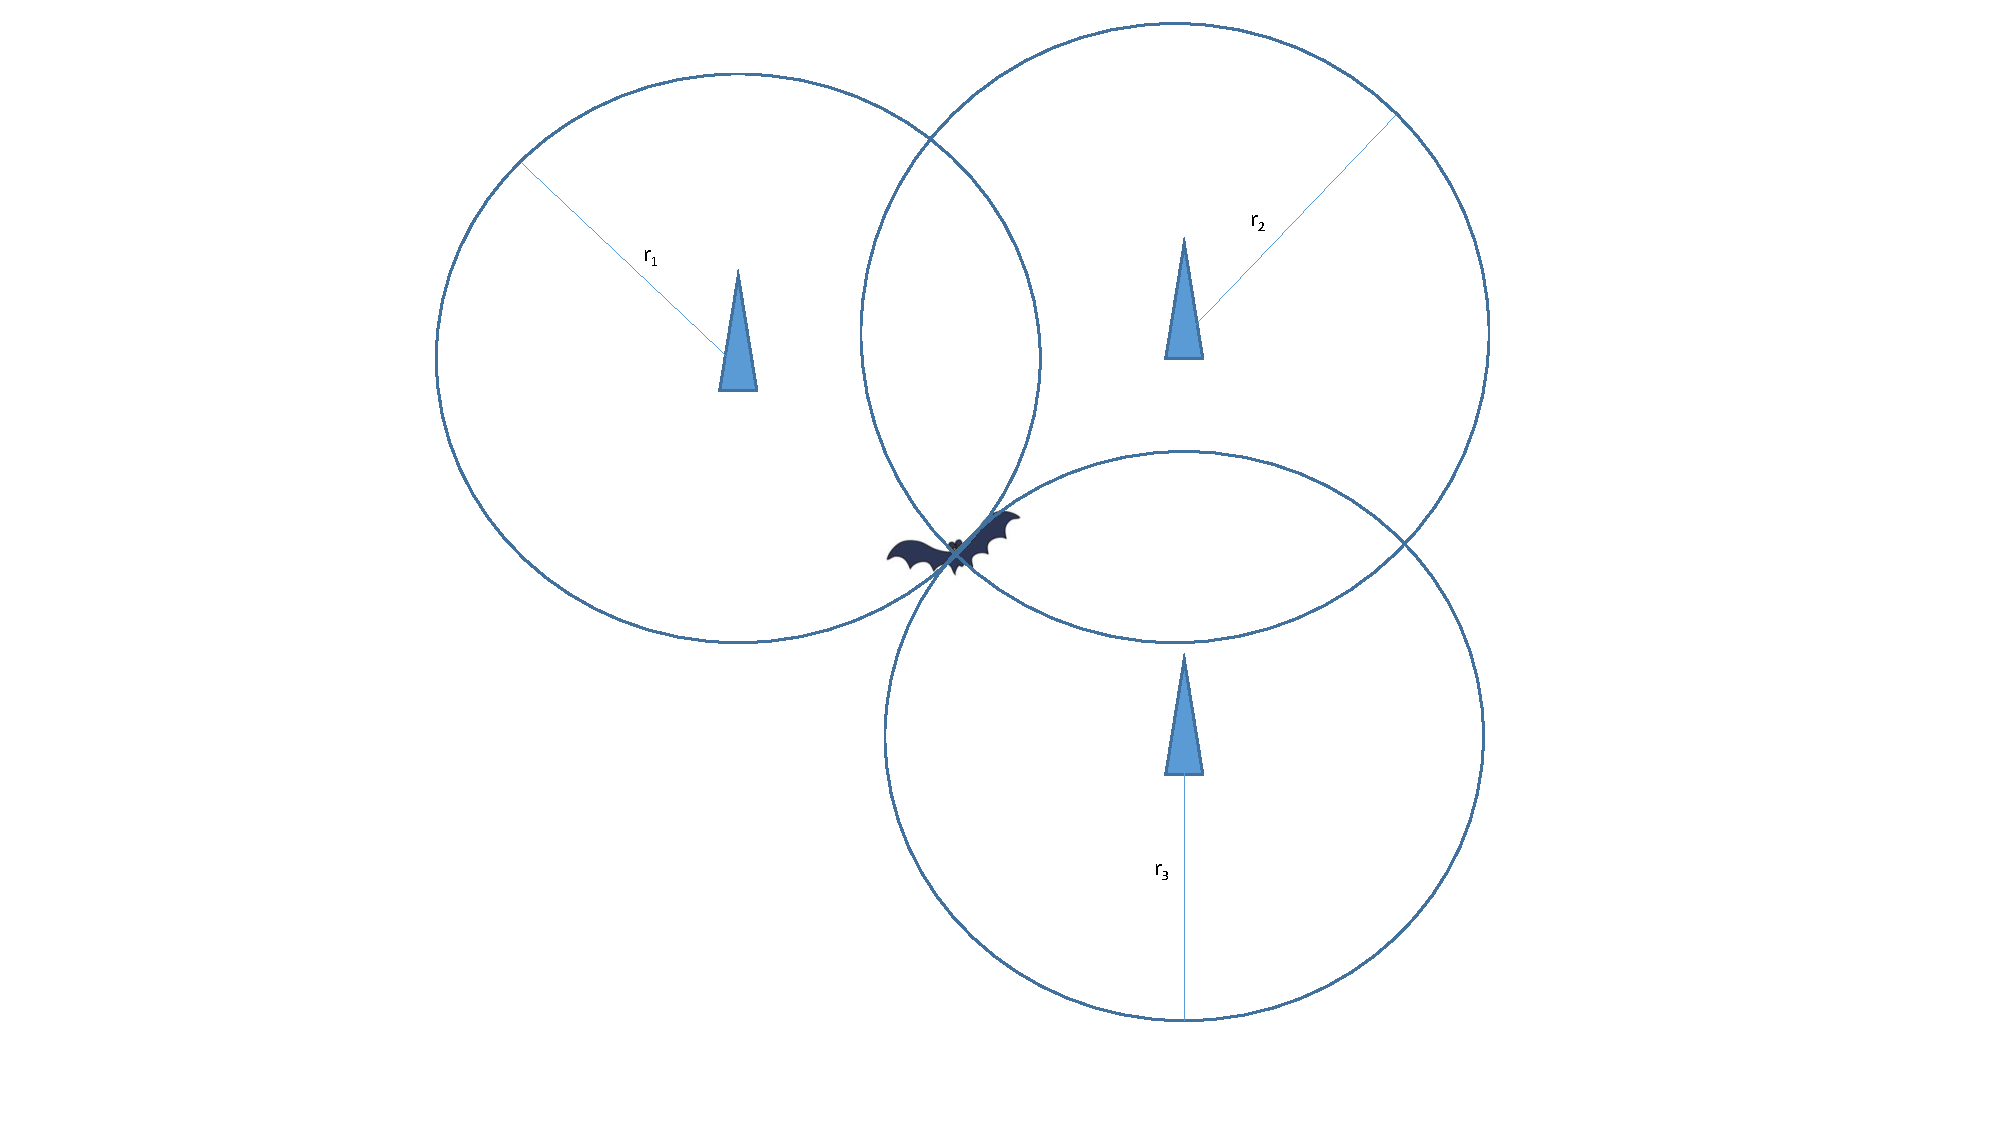
\includegraphics[width = \textwidth]{images/Trilateration}
 \caption{Trilateration}
 \label{fig:Trilateration}
\end{figure}

Ob mit dieser Methode eine hohe Genauigkeit erzielt wird, hängt davon ab, wie fehlerbehaftet die Distanzmessungen sind. Die Distanz lässt sich aus zwei unterschiedlichen Messungen gewinnen. Zum einen kann man die Signalleistung, zum anderen die Laufzeit auswerten. 
Mit Kenntnissen der Ausbreitungsdämpfung und der Sendesignalleistung ist es möglich, auf eine Distanz, die die Welle zurückgelegt haben muss, zu schließen. 

Mithilfe der Laufzeit \gls{symb:tau} und Ausbreitungsgeschwindigkeit \gls{symb:c0}\footnote{Die Ausbreitungsgeschwindigkeit einer elektromagnetischen Welle, entspricht im Vakuum der Lichtgeschwindigkeit, ist sonst aber materialabhängig.} einer elektromagnetischen Welle, ist es ebenfalls möglich die Distanz zu berechnen.

\begin{equation}
	\label{eq:Distanzberechnung}
	r = c_0\cdot \tau
\end{equation}

Die Schwierigkeit besteht darin, die Laufzeit, über einen stark gestörten Kanal, möglichst genau zu ermitteln. 

\section{Laufzeitschätzung}
\label{chap2.1:Laufzeitschätzung}
Möglichkeiten zur Ermittlung der Laufzeit beruhen auf den Ausbreitungsgesetzen elektromagnetischer Wellen. Diese lassen sich aus den Maxwell-Gleichungen, welche die Eigenschaften elektromagnetischer Felder und deren Ausbreitung beschreiben, ableiten.
Die Bestimmung der Laufzeit einer Welle, lässt sich jedoch auch Systemtheoretisch ausdrücken. Die räumliche Ausbreitung der Welle wird dabei als zeitliche Verzögerung eines Signals betrachtet. Dabei korrespondiert eine Verzögerung im Zeitbereich mit einer Phasenmodulation im Frequenzbereich. Der Verschiebungssatz der Fouriertransformation zeigt diesen Zusammenhang: 

\begin{equation}
	\label{eq:Verschiebungssatz}
	x(t - \tau) \; \laplace\; X(f)e^{-j2 \pi f_c \tau}
\end{equation}


Wenn die Trägerfrequenz \gls{symb:fc} und die Phasendrehung $\gls{symb:phi}=2\pi  \gls{symb:fc}\gls{symb:tau}$ bekannt sind, kann die Verzögerung \gls{symb:tau} bestimmt werden. 
Da die Phasendrehung aber periodisch mit der Periode $2\pi$ ist, kann keine eindeutige Aussage über die Laufzeit getroffen werden. Um das an einem Zahlenbeispiel zu verdeutlichen, soll von einem Signal mit der Frequenz \unit[1]{GHz} ausgegangen werden. Dieses Signal hat eine Periodendauer von \unit[1]{ps}. Nach \eqref{eq:Distanzberechnung} entspricht das einer Strecke von \unit[30]{cm}. Nach diesen \unit[30]{cm} wiederholt sich die Phase. Damit kann die zurückgelegte Strecke nur auf den ersten \unit[30]{cm} eindeutig bestimmt werden, da man danach nicht genau sagen kann, in welcher Periode man sich befindet. Damit ist der Eindeutigkeitsbereich der Phaseninformation der Welle auf einen Bereich von \unit[30]{cm} beschränkt. Je höher die Frequenz, desto kleiner ist der Eindeutigkeitsbereich. Dieser Bereich kann jedoch vergrößert werden, indem Phasendifferenzen verwendet werden. Dazu werden Signale mit mehreren Frequenzanteilen, sogenannte Subträger, erzeugt. Die Geschwindigkeit, mit der sich die Phase dreht, wird mit dem Phasenmaß \gls{symb:beta} $= \omega \sqrt{\epsilon \mu}$ angegeben, wobei \gls{symb:omega} der Kreisfrequenz und \gls{symb:epsilon} und \gls{symb:mu} den Materialeigenschaften entsprechen. Aus diesem Zusammenhang ist erkennbar: je höher die Frequenz, desto schneller dreht sich die Phase. Die hieraus resultierende Phasendifferenz \gls{symb:dphi} zwischen den, bei unterschiedlichen Frequenzen liegenden Subträgern, wird zur Laufzeitbestimmung verwendet. 
Je länger die Welle wandert, desto größer wird die Differenz, aufgrund der unterschiedlichen Drehgeschwindigkeiten. Allerdings ist auch der Eindeutigkeitsbereich dieser Methode begrenzt, da die Phasendifferenz selbst periodisch ist. Die Länge der Periodendauer ist vom Abstand der Subträger zueinander abhängig. Bei einem großen Abstand erfolgt die Verdrehung zueinander schneller und führt damit zu einer kürzeren Periodendauer. Somit verhält sich der Eindeutigkeitsbereich $\gls{symb:tau}_{max}$ umgekehrt proportional zum Frequenzabstand \gls{symb:df}.

\begin{equation}
	\label{eq:Eindeutigkeitsbereich}
	\tau_{max} = \frac{1}{\Delta f}
\end{equation} 

Wenn man das zuvor genannte Beispiel wieder heranzieht, und von einer Mittenfrequenz bei \unit[1]{GHz} und einer Bandbreite von \unit[2]{MHz} ausgeht, ist der größtmögliche Subträgerabstand \gls{symb:df} gleich der Bandbreite. Als kleinstmöglichen Eindeutigkeitsbereich ergeben sich \unit[150]{m}. 
Für die Laufzeitbestimmung muss die gemessene Phasendifferenz in Bezug zum jeweiligen Subträgerabstand gestellt werden, da der Abstand maßgeblich für die Stärke der Verdrehung verantwortlich ist.
Aus diesem Zusammenhängen, und aus den Gleichungen \eqref{eq:Distanzberechnung} und  \eqref{eq:Verschiebungssatz}, folgt für die Distanzschätzung mittels Phasendifferenzen folgende Beziehung \citep{nowak2014system}:

\begin{equation}
	\label{eq:Phasendifferenz}
	r = \frac{c_0}{2\pi}\cdot\frac{\partial\varphi}{\partial f}
\end{equation}

Die Ableitung der Phase nach der Frequenz entspricht einer Gruppenlaufzeit. Diese beschreibt wie lange eine Wellengruppe (mehrere Subträger) gewandert ist. 


\section{Kanalmodell}
\label{chap2.2:Kanalmodell}
Wenn die Phasen exakt gemessen werden können, ermöglicht dies eine sehr genaue Bestimmung der Laufzeit im Eindeutigkeitsbereich. Beim Detektieren von Signalen passieren jedoch häufig Fehler. Diese entstehen aufgrund von Störeinflüssen der Umgebung. Damit der Einfluss dieser Fehlerquellen verringert werden kann, muss der Übertragungskanal genauer untersucht werden. Wenn das Übertragungsverhalten des Kanals bekannt ist, können anschließend Signale und Schätzverfahren entworfen werden, um Störeinflüsse zu minimieren.   
Um Einflüsse der Umgebung zu simulieren, wird ein mathematisches Modell benötigt, welches diese beschreibt. Dabei werden die unterschiedlichen Störungen getrennt betrachtet und am Ende zusammengeführt. Die Laufzeit der Welle wird als Verzögerungsglied modelliert, welches die Phasendrehung realisieren soll.

\subsection{Additiv White Gaussian Noise (AWGN) - Kanal}
\label{chap2.2.1:AWGN}
Zunächst kann von einem \gls{AWGN}-Kanal, wie in Abbildung \ref{fig: AWGN-Kanal} ausgegangen werden. Ein solches Rauschmodell, stellt den "`\emph{worst case}"' dar, da das gesamte Band konstant verrauscht ist. Dieser Kanal addiert auf das verzögerte Sendesignal $s(t-\tau)$ eine Musterfunktion $n(t)$ aus einem Gaußschen Rauschprozess $N$ mit einem konstanten Leistungsdichtespektrum $\Phi(f) = \frac{N_0}{2}$, sodass das Empfangssignal $r(t)$ resultiert. Eine Musterfunktion entspricht einer konkreten Realisierung eines Zufallsprozesses. 

\begin{figure}[htbp]
\centering
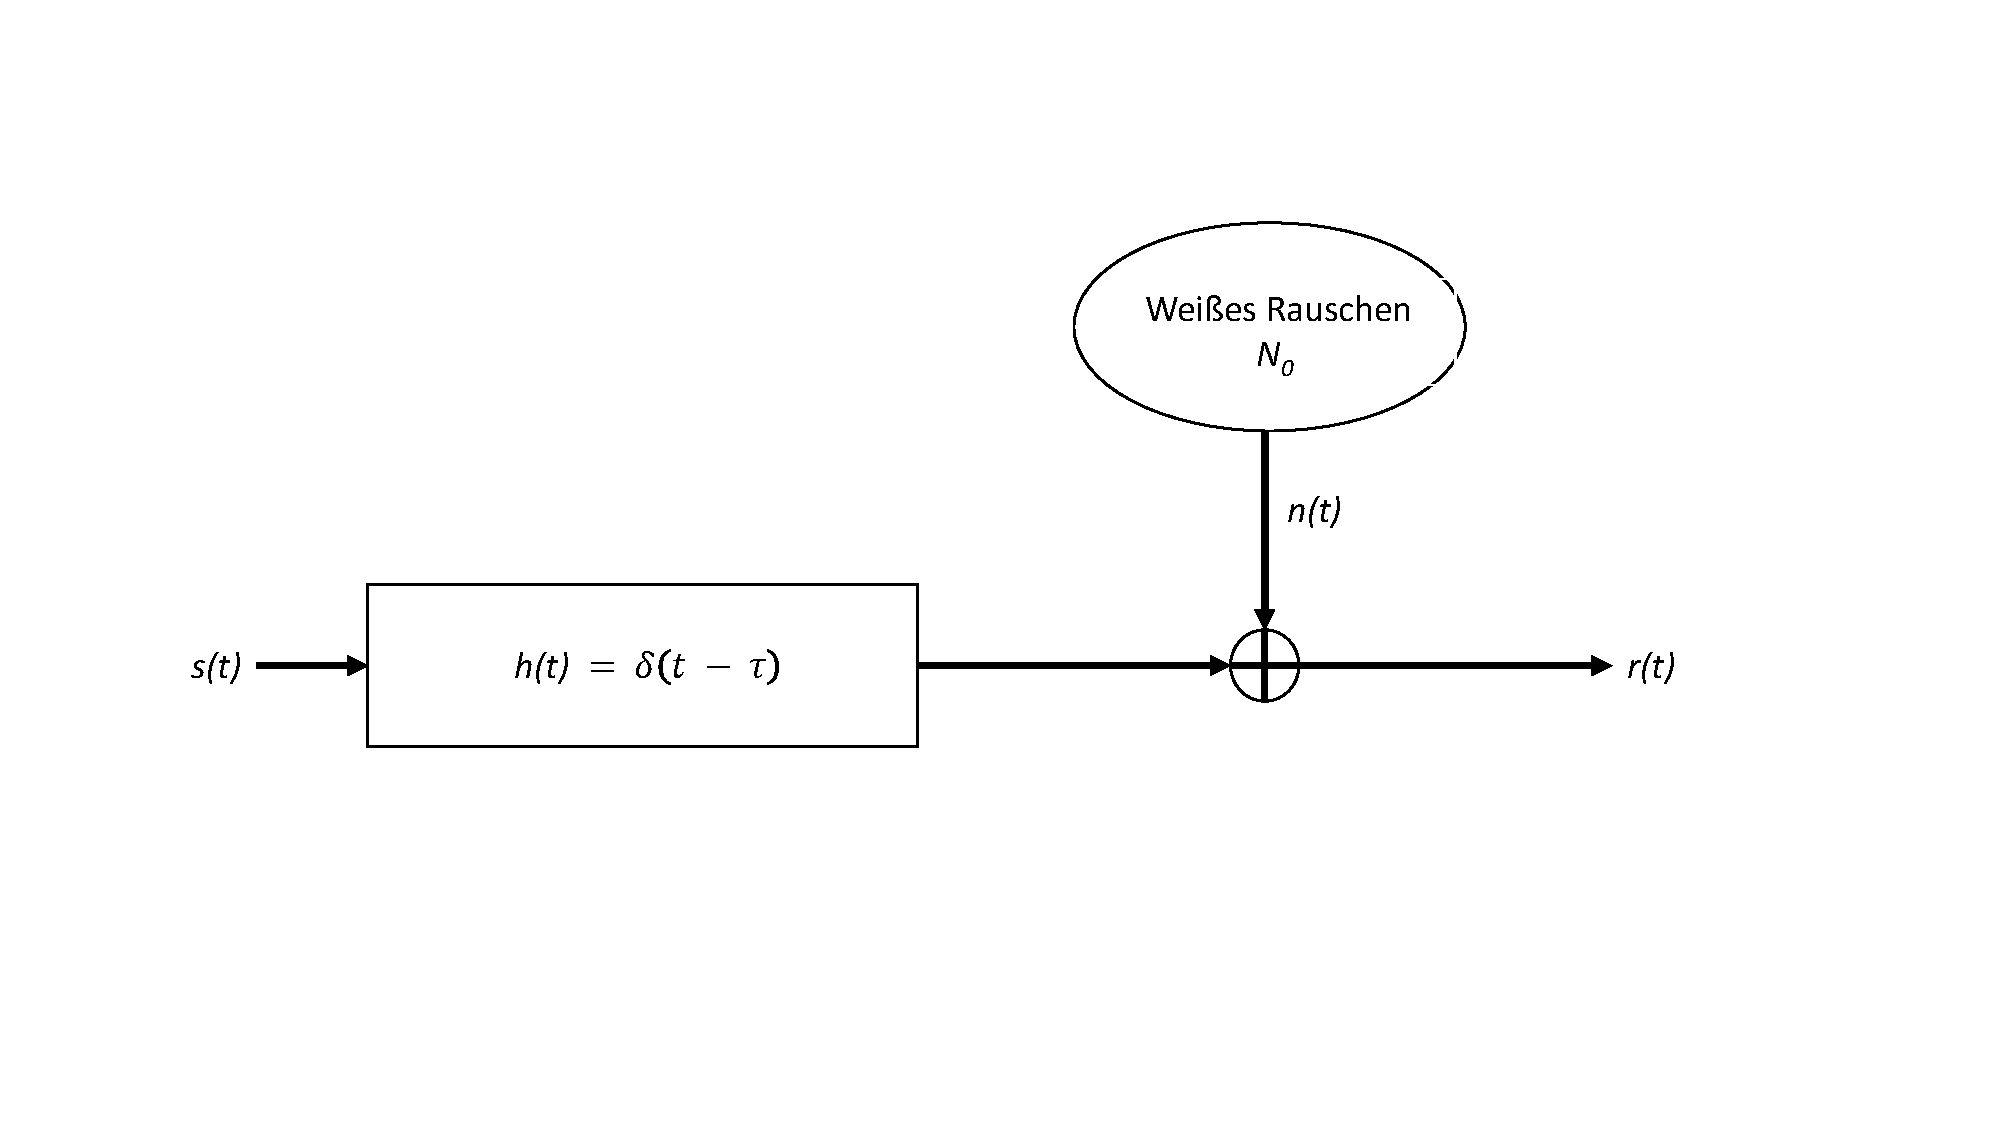
\includegraphics[width = \textwidth]{images/WeisesRauschen}
\caption{Blockschaltbild zu einem AWGN-Kanal}
\label{fig: AWGN-Kanal}
\end{figure}

Wie im vorherigen Kapitel bereits angesprochen, führt das Verzögerungsglied zu einer frequenzabhängigen Phasendrehung. Für eine feste Laufzeit ergibt sich, aufgrund des linearen Zusammenhangs zwischen Phasendrehung und Laufzeit aus \eqref{eq:Verschiebungssatz}, eine Rampe mit der Steigung $2\pi\tau$. Vernachlässigt man die Dämpfung, ist der Betragsgang der Übertragungsfunktion $H(f)$ konstant gleich eins. Die Aufgabe, der in dieser Arbeit vorgestellten Schätzverfahren, ist es, die Steigung der Phasenrampe zu ermitteln. Deshalb ist von großem Interesse, welchen Einfluss der \gls{AWGN}-Kanal auf den Phasengang des Verzögerungsgliedes hat.  In Abbildung \ref{fig: AWGN-Plot}, wurde ein solcher Kanal simuliert. Auf der rechten Seite ist der Phasengang und auf der Linken der Betragsgang eines solchen Kanals zu sehen. Durch additives Rauschen ist der Phasengang ebenfalls verrauscht, wobei es vom Signal-Rausch-Verhältnis (\gls{SNR}) abhängt, wie groß die Schwankungen sind. Bei einer Schätzung der Phasendifferenz mit zwei Trägern, werden zwei Werte aus diesem Verlauf entnommen und versucht daraus die Steigung zu ermitteln.

\begin{figure}[htbp]
	\centering
	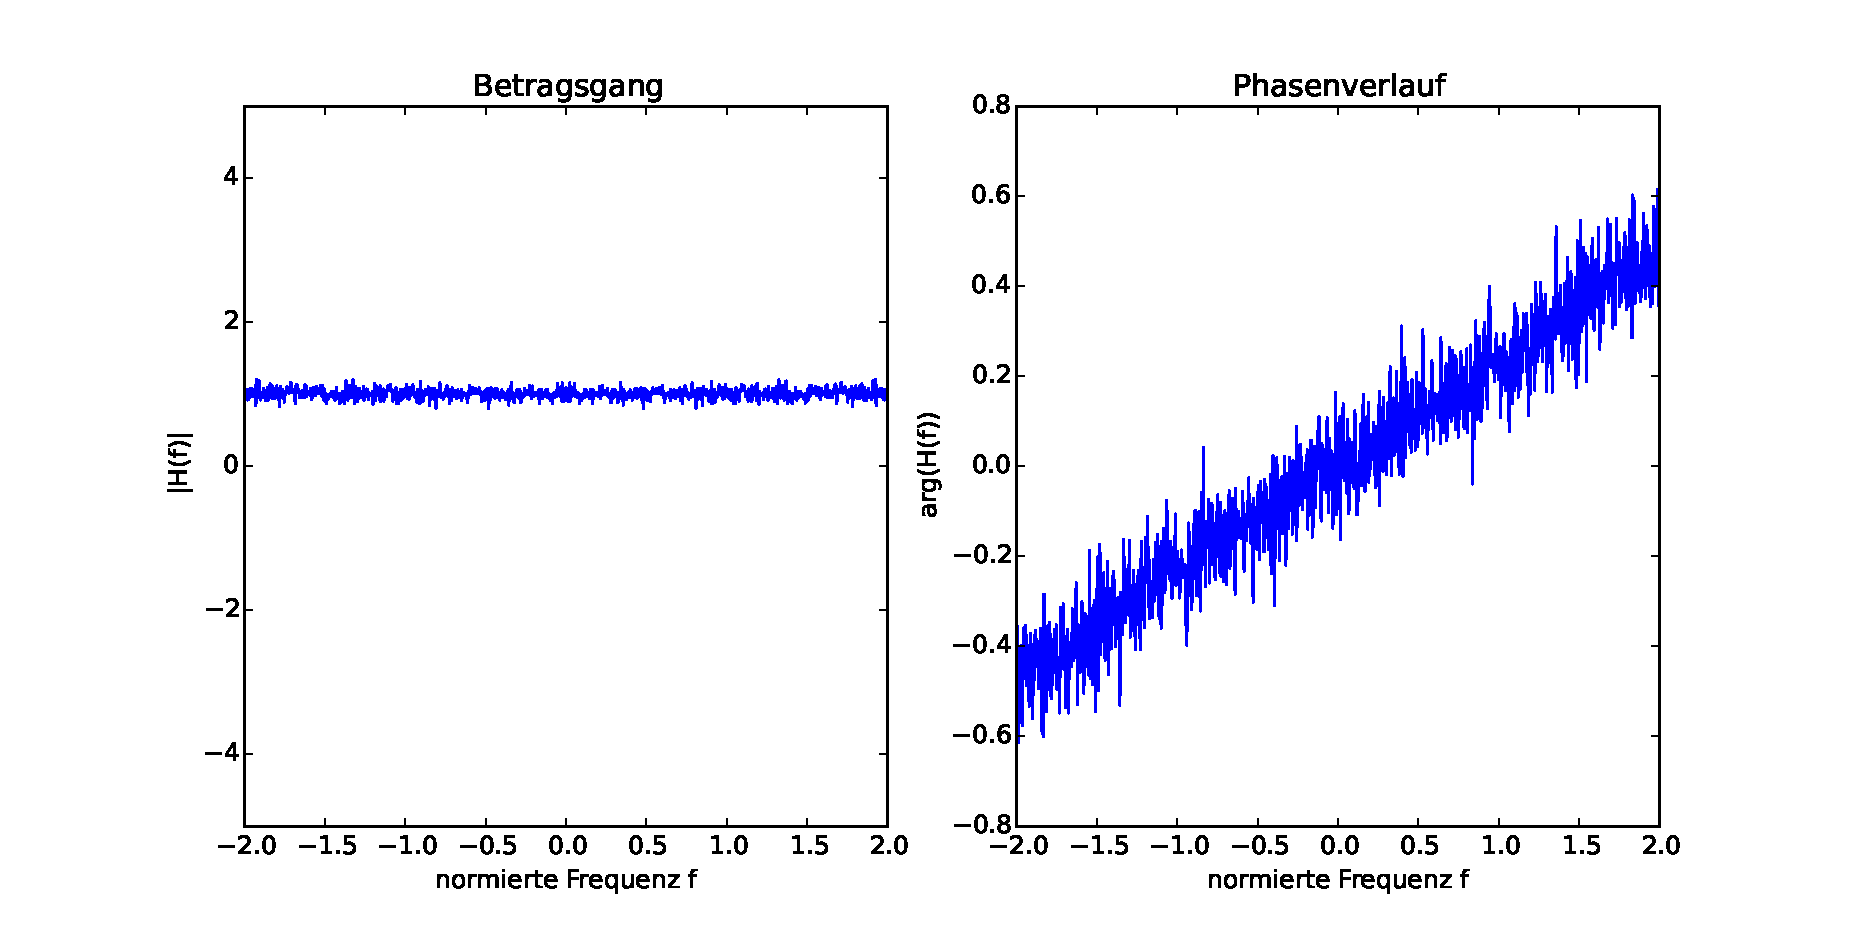
\includegraphics[width=\textwidth]{images/AWGN}
	\caption{Übertragungsverhalten eines \gls{AWGN}-Kanals}
	\label{fig: AWGN-Plot}
\end{figure}

\subsection{Mehrwegeausbreitung}
\label{chap2.2.2:Mehrwege}
Ein weiterer Störeinfluss ist die Mehrwegeausbreitung. Das Signal erreicht nicht nur über die Sichtverbindung (\gls{LOS}) das Ziel, sondern wird an Objekten in der Umgebung reflektiert und gestreut. Diese gestreuten Signalanteile überlagern sich am Empfänger mit dem \gls{LOS}-Signal additiv. Das \gls{LOS}-Signal ist dann nicht mehr klar von den Umwegpfaden trennbar. Ein solcher Kanal kann durch mehrere parallele  Verzögerungsglieder modelliert werden. Diese werden mit einem Dämpfungsfaktor $\alpha_i$ gewichtet und aufgrund der Beschaffenheit der Reflektoroberfläche zusätzlichen in der Phase gedreht, was durch einen komplexen Zeiger $\e^{j\Phi_i}$ modelliert werden kann. Je nach Anzahl $L$ und Gewichtung $\alpha_i$ der Umwegpfade, ist die Phase mehr oder weniger stark verfälscht. Für die Impulsantwort des Kanals ergibt sich daher folgender Ausdruck:

\begin{equation}
	\label{eq:Mutipath}
	h(t) = \sum_{i = 0}^L \, \alpha_i \, \delta(t - \tau_i)\, e^{j\Phi_i} \;\;\laplace\;\; H(f) =  \sum_{i = 0}^L \, \alpha_i \, e^{-j2\pi f \tau_i + \Phi_i}
\end{equation}

Um die Komplexität des Kanalmodells nicht zu groß werden zu lassen, sollen in dieser Arbeit zunächst nur Betrachtungen mit einem Umwegpfad gemacht werden.
In Abbildung \ref{fig:MehrwegeZeiger} ist veranschaulicht, wie sich die Phase zweier additiv überlagerter komplexer Zeiger verhält. Der in rot dargestellte, mit $\alpha$ skalierte Vektor des Umwegpfades dreht mindestens bis $\varphi_{LOS}$, da die Sichtverbindung der kürzest mögliche Pfad ist. 

\begin{figure}[htbp]
	\centering
	\hspace*{2cm}
	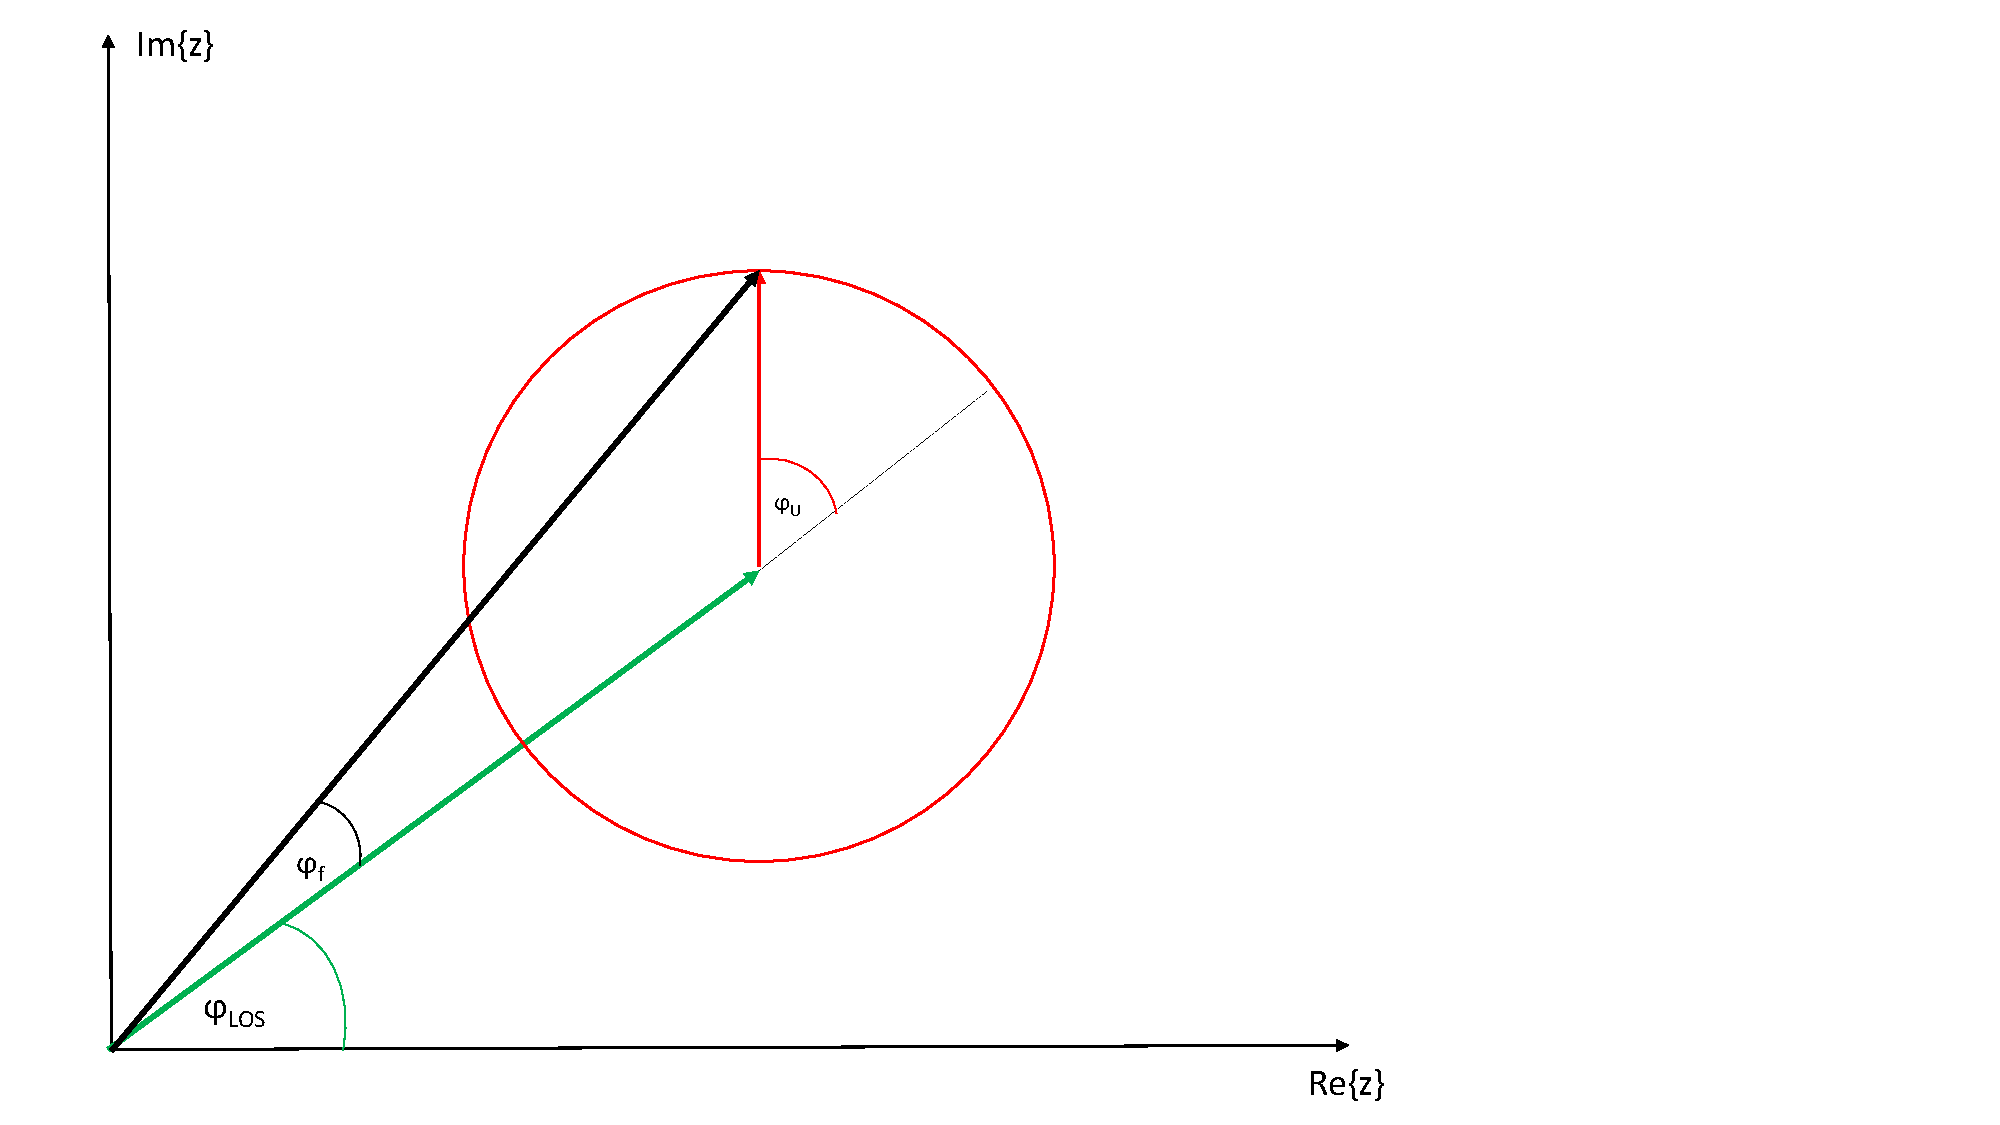
\includegraphics[width = \textwidth]{images/MehrwegZeiger}
	\caption{Zwei additiv überlagerte komplexe Zeiger}
	\label{fig:MehrwegeZeiger}
\end{figure}

Abhängig von der Länge des Umwegpfades, dreht er sich um $\varphi$\textsubscript{u} weiter. Der in der Abbildung \ref{fig:MehrwegeZeiger} schwarze, resultierende Vektor, hat nun eine, um $\varphi$\textsubscript{f} von $\varphi$\textsubscript{LOS} abweichende Phase. Wenn sämtliche Umwege betrachtet werden, dreht sich der Umwegvektor auf einem Kreis um die Spitze des LOS-Vektors. $\varphi$\textsubscript{f} schwingt dabei sinusartig um $\varphi$\textsubscript{LOS}, wobei die Amplitude dieser Schwingung von dem Skalierungsfaktor $\alpha$ abhängt. Ein Sonderfall entsteht bei $\alpha = 1$. Hier entspricht die Amplitude des Umwegpfades der des LOS-Pfades und sorgt bei einem $\varphi$\textsubscript{u} von $180^\circ$ für einen Phasensprung. In diesem Fall verhält sich $\varphi$\textsubscript{f} wie ein Sägezahn um $\varphi$\textsubscript{LOS} \cite{mehrwegeausbreitung}.


\begin{figure}[htbp]
	\centering
	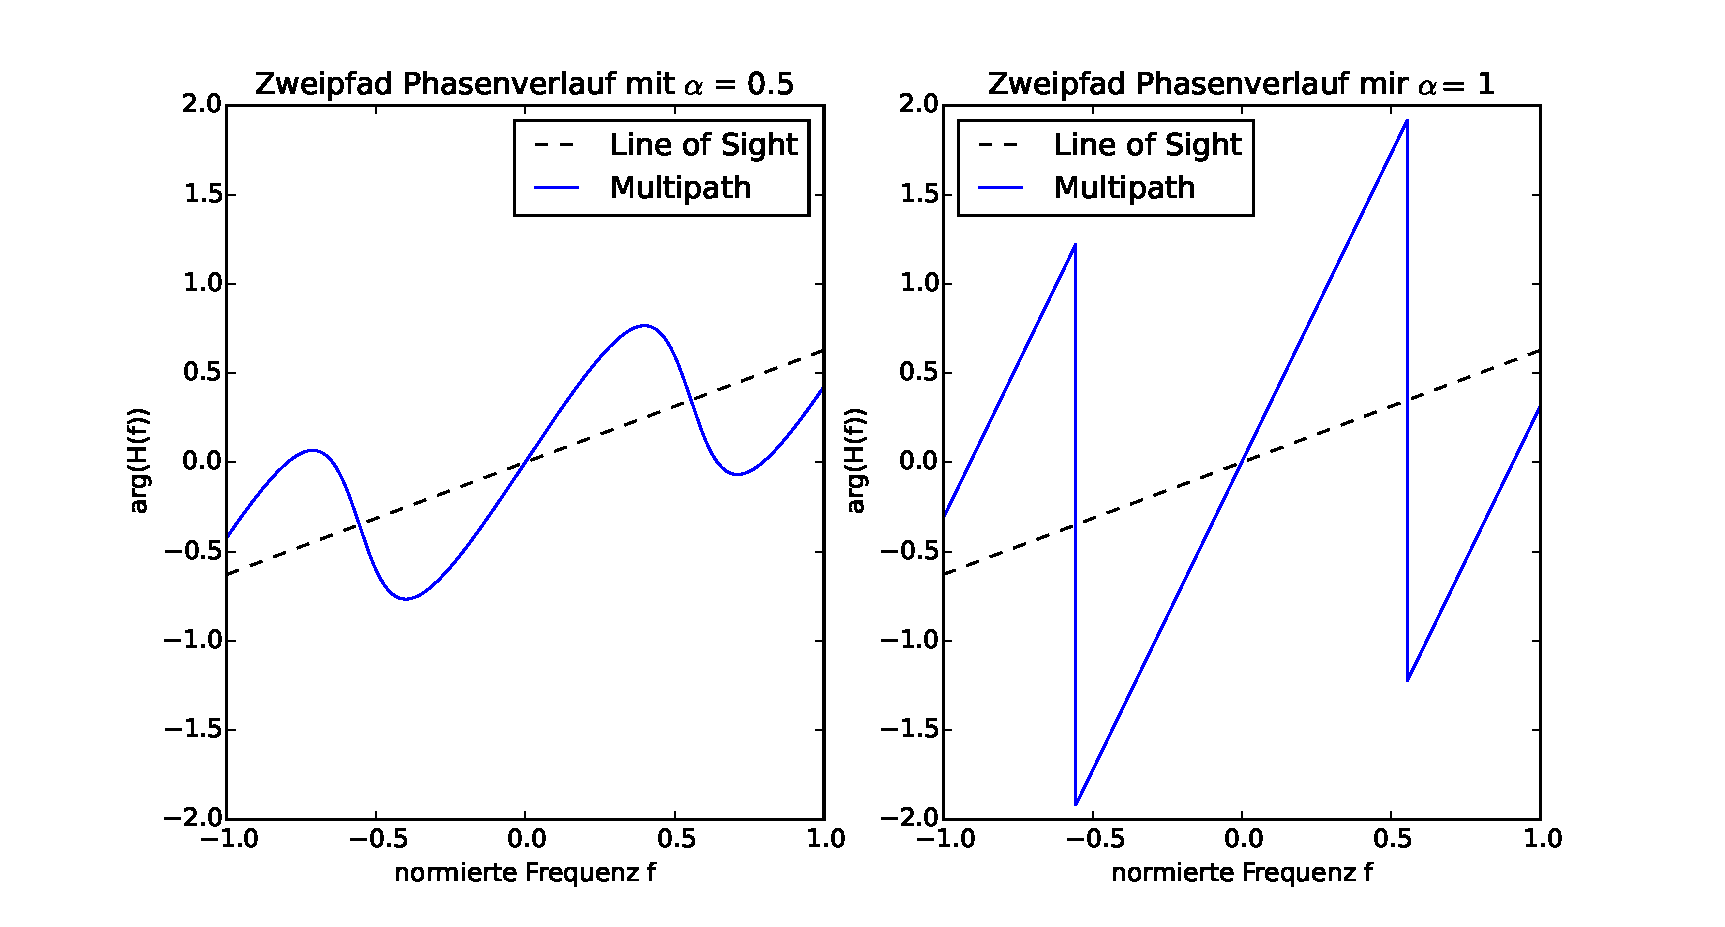
\includegraphics[width=\textwidth]{images/MutipathSim}
	\caption{Phasenverlauf eines Zweipfadkanals}
	\label{fig:MutipathSim}
\end{figure}

In Abbildung \ref{fig:MutipathSim} wurde beispielhaft ein solcher Phasenverlauf eines Zweipfadkanals simuliert. Auf der linken Seite ist die sinusförmige Schwingung um die eigentliche Phasenrampe und auf der Rechten der Sägezahn zu erkennen.
In Abbildung \ref{fig:MehrwegeZeiger} ist zu sehen, dass die Amplitude des Signals nicht unberührt vom zweiten Pfad bleibt. Teilweise trägt der Umweg konstruktiv, teilweise auch destruktiv zur Amplitude bei. Dabei kann es sogar zur völligen Auslöschung des Zeigers kommen. Dies führt bei einer Multiplikation mit dem Signal zu einer Auslöschung des Subträgers. Ein solcher Kanal wird deshalb auch frequenzselektiver Fadingkanal genannt, da, je nach Umweglänge, unterschiedliche Frequenzen stark gedämpft werden. In Abbildung \ref{fig:MutipathSim_abs} wird der Betragsgang zum obigen Phasenverlauf aufgezeigt, anhand dessen der frequenzselektive Schwund an zwei Stellen im Band erkennbar wird. In diesem Beispiel wäre die Bestimmung der Phasendifferenz nicht mehr möglich, wenn genau diese Stellen mit Subträgern belegt worden wären. All diese Eigenschaften lassen darauf schließen, dass eine geringe Anzahl von Subträgern für die Phasendifferenzbestimmung sehr anfällig für den Mehrwegekanal sind. Diese Erkenntnis gibt einen Hinweis darauf, wie Signale entworfen werden müssen, damit sie möglichst robust gegenüber den Einflüssen des Kanals sind: Je mehr Subträger das Signal hat, desto besser lässt sich der Kanal auflösen. 

\begin{figure}[htbp]
	\centering
	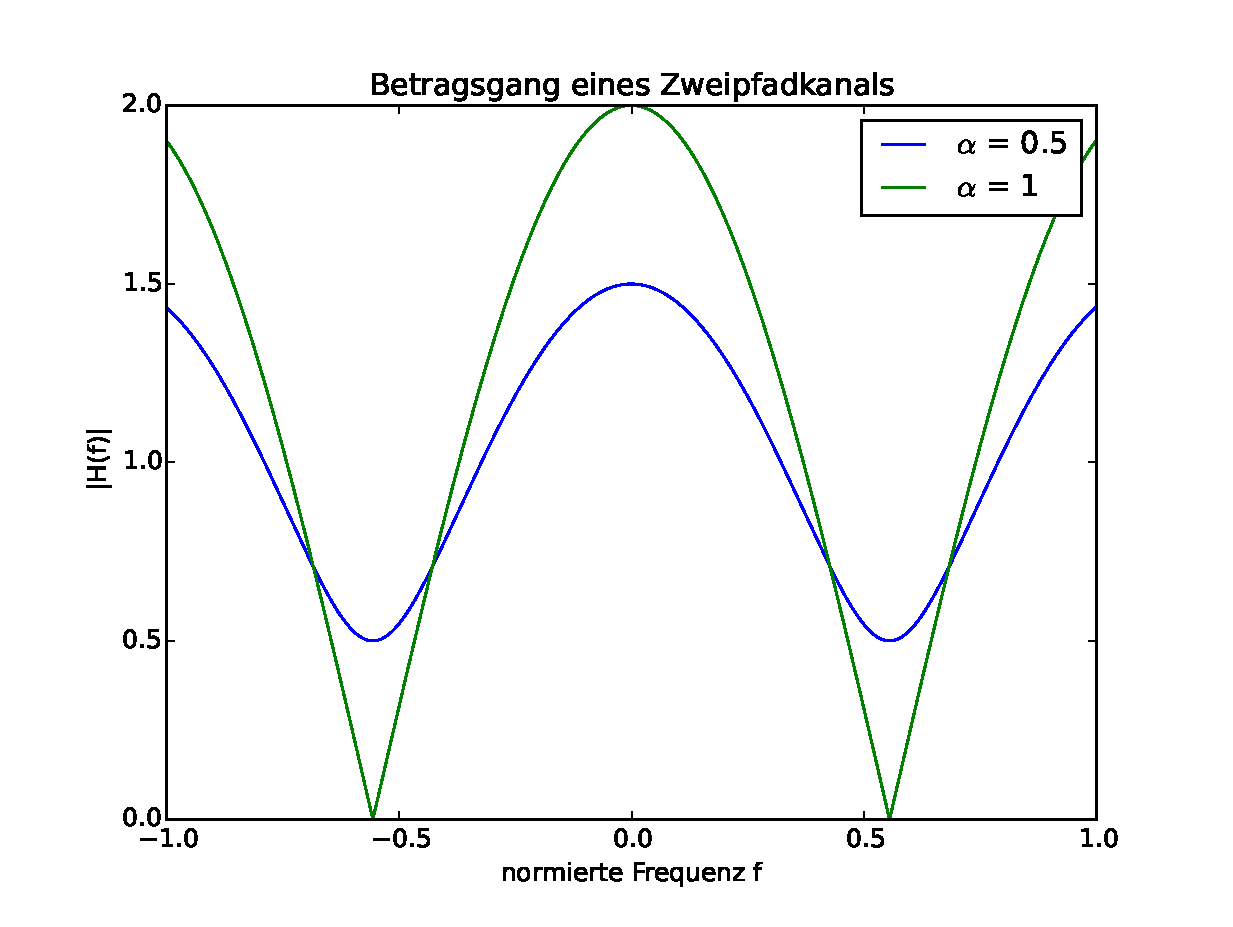
\includegraphics[scale=0.5]{images/MutipathSim_abs}
	\caption{Betragsgang eines Zweipfadkanals}
	\label{fig:MutipathSim_abs}
\end{figure}

\section{Schätztheorie}
\label{chap2.3:Schätztheorie}
Aus dem Kanalmodell wird ersichtlich, dass Signale mit einem weißen Spektrum weniger anfällig gegenüber den Einflüssen des Mehrwegekanals wären, da die Fehleinflüsse frequenzselektiv sind. Die Eigenschaften, die ein Signal benötigt, um Schätzfehler unter Einfluss eines \gls{AWGN}-Kanals zu minimieren, sind jedoch noch nicht offensichtlich. Die Schätztheorie beschäftigt sich damit, wie die Parameterschätzung bei gestörten Größen verbessert werden kann. Im Folgenden sollen einige Erkenntnisse der Schätztheorie genauer erläutert werden, um verständlich zu machen, wie ein Schätzer und das Signal aufgebaut sein müssen damit möglichst wenig Fehler verursacht werden. 

Die Aufgabe besteht darin, aus einer Reihe von Beobachtungswerten $x$ einen unbekannten Parameter $\theta$ zu schätzen. 
Um einen Schätzer zu entwerfen, muss zunächst ein mathematisches Modell, zum Beschreiben der Beobachtungswerte gefunden werden. Da diese Werte zufällig sind, werden sie durch ihre \gls{WDF} $p(x;\theta)$ beschrieben. Diese wird, durch die zu schätzende Größe $\theta$, parametrisiert. Die Funktion $p(x;\theta)$ ist zunächst unbekannt und muss aus den Gegebenheiten, z.B. dem Kanalmodell, bestimmt werden.  Bei einem \gls{AWGN}-Kanal handelt es sich um eine Gaußverteilung mit Varianz $\sigma^2$ und Mittelwert $\theta$. 

\begin{equation}
	\label{eq:gaussverteilung}
	p(x;\theta) = \frac{1}{\sqrt{2\pi\sigma^2}} \; e^{-\frac{(x-\theta)^2}{2\sigma^2}}
\end{equation}

Sobald eine solche \gls{WDF} spezifiziert wurde, besteht die Aufgabe darin einen optimalen Schätzer, und somit eine  Abbildung der Beobachtungswerte auf den jeweiligen Parameterwert, wie in \eqref{eq:Schätzabbildung} zu finden, welcher einen möglichst geringen Fehler macht. 

\begin{equation}
	\label{eq:Schätzabbildung}
	\hat{\theta} = g(x[0],x[1],x[2]...,x[N-1])
\end{equation} 

Bei jedem zu schätzenden Parameter gibt es zwei Varianten. Der eigentliche Parameterwert $\theta$, welcher unbekannt ist und der Schätzwert $\hat{\theta}$.
Da die Werte $x$ aus einer Zufallsvariablen $X$ entstanden sind, müssen die Schätzwerte $\hat{\theta}$ auch zufällig sein. Aus diesem Grund können diese nur mit statistischen Mitteln, wie Erwartungswert $E[\;]$ und Varianz $Var(\;)$, evaluiert werden. 
Schätzer können in drei Klassen eingeteilt werden:

\begin{enumerate}
	\item erwartungstreue Schätzer (unbiased estimator): $E[\hat{\theta}(X)] = \theta$
	\item Schätzer mit bekannter Ablage B (biased estimator): $E[\hat{\theta}(X)] = \theta + bias$
	\item Schätzer mit unbekannter Ablage B($\theta$):  $E[\hat{\theta}(X)] = \theta + bias(\theta)$
\end{enumerate}

 Um einen Schätzer zu optimieren, wäre der erste Gedanke den mittleren quadratischen Schätzfehler zu minimieren. Der \gls{mse} ist definiert durch 
 
\begin{equation}
	\label{eq:MSE}
	mse(\hat{\theta}) = E \left[(\hat{\theta} - \theta)^2\right] = var(\hat{\theta}) + bias^2(\theta)
\end{equation}  

Nach \cite[S.19]{kay1993fundamentals} besteht dieser aus der Varianz des Schätzwertes und der Ablage zum Quadrat. Damit man diesen Ausdruck minimieren kann, muss die Ablage bekannt sein. Diese ist allerdings vom zu schätzenden Parameter $\theta$ selbst abhängig. Deshalb ist es nur möglich einen \emph{minimum}-\gls{mse}-\emph{estimator} zu finden, wenn die Ablage bekannt ist. Dies ist meistens jedoch nicht der Fall. Wenn der Schätzer keine Ablage hat, ist es möglich die Varianz zu minimieren. Ein solcher Schätzer nennt sich dann  \gls{mvue}. Dieser Schätzer existiert nicht immer. Falls ein solcher Schätzer existiert, gibt es jedoch auch keine Methodik ihn sicher zu finden\cite[S.20f.]{kay1993fundamentals}. 

\subsection{Cramer Rao Lower Bound}
\label{chap2.3.1:CRLB}
Möglich ist es aber, eine untere Schranke für die Varianz des Fehlers zu berechnen. Eine solche Schranke ermöglicht es Schätzer mit ihr zu vergleichen. Wenn die Fehlervarianz des Schätzers auf der Schranke liegt, wurde der \gls{mvue} gefunden. Diese Schranke nennt sich \gls{CRLB} (deutsch: Cramer-Rao-Schranke). Im folgenden Kapitel wird ihre Berechnung genauer erläutert.

Ausgangspunkt ist die \gls{WDF}. Wenn diese Funktion vom Parameter $\theta$ abhängig ist und eine Wahrscheinlichkeitsdichteverteilung für den Beobachtungsvektor $x$ liefert, wird sie als Likelihood-Funktion bezeichnet. Ein Maximum-Likelihood-Schätzer wird versuchen über alle Parameter $\theta$ diese Funktion zu maximieren, um somit einen Schätzwert $\hat{\theta}$ zu finden. Wenn diese Funktion besonders steil verläuft, wie in Abbildung \ref{fig:ML_Herleitung} auf der linken Seite angedeutet, und ein eindeutiges Maximum hat, ist dessen Angabe mit geringerer Abweichung möglich. 

\begin{figure}[htbp]
	\centering
	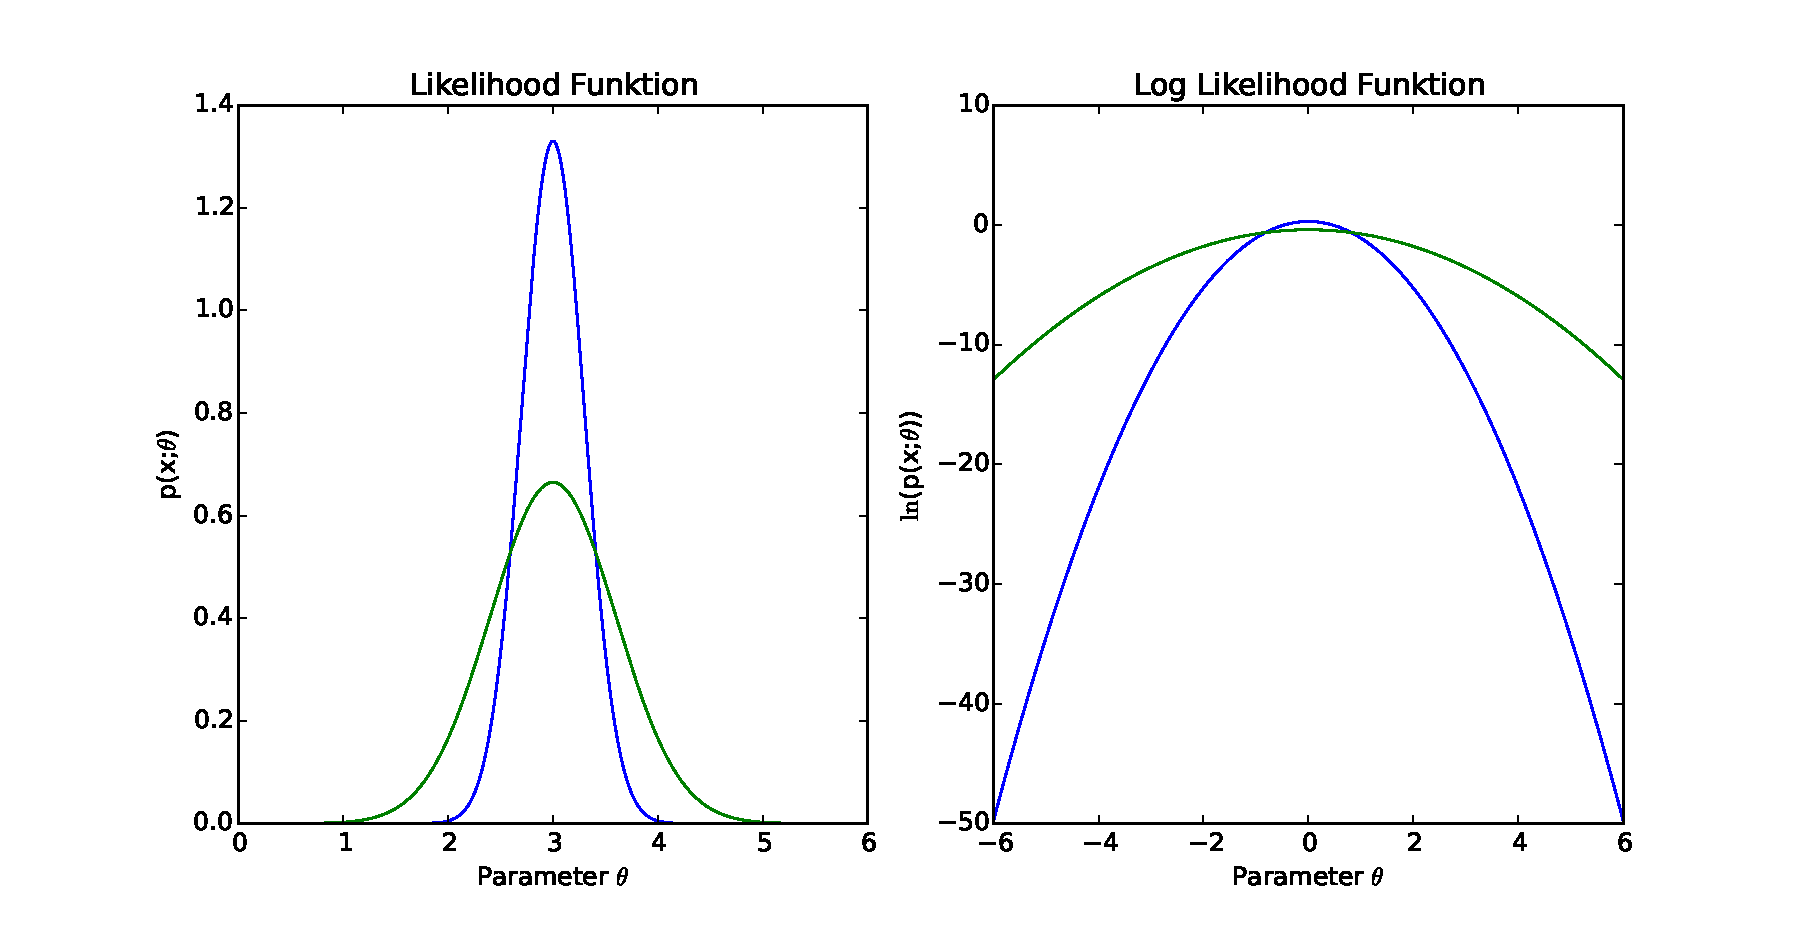
\includegraphics[width = \textwidth]{images/ML_Herleitung}
	\caption{Maximum-Likelihood- und Log-Likelihood Funktion für unterschiedliche $\sigma$}
	\label{fig:ML_Herleitung}
\end{figure}

Die blau Kurve ist eine Normalverteilung mit sehr kleiner Varianz $\sigma^2$. Da die Varianz der grünen Kurve größer ist, ist die Funktion flacher. Die Werte um das Maximum der grünen Kurve, bilden auf einen größeren Parameterbereich ab. Daher erzeugt ein verfehlen des Maximums einen größeren Parameterfehler. Wenn die Kurve steil verläuft, wie bei der Blauen, wird auf einen wesentlich kleineren Parameterbereich abgebildet. Somit hält sich der Schätzfehler, beim verfehlen des Maximums in grenzen. Das bedeutet somit auch, dass die Steilheit der Likelihood-Funktion ein Maß dafür ist, wie genau man den gesuchten Parameter schätzen kann. Diese Steilheit kann über die Krümmung der Log-Likelihood-Funktion quantifiziert werden\cite[S.29]{kay1993fundamentals}. Die Krümmung nimmt mit steigender Steilheit zu und berechnet sich nach \eqref{eq:Curvature}. 

\begin{equation}
	 \label{eq:Curvature}	
	 -E \left[\frac{\partial^2 \ln p(x;\theta)}{\partial \theta^2} \right]
\end{equation}

Aus dieser Beziehung wird ersichtlich, dass die Varianz proportional zur Inversen der Krümmung der Log-Likelihood-Funktion ist. Sie gibt die bestmögliche Genauigkeit einer Schätzung an und bildet deshalb eine untere Schranke.

\begin{equation}
	\label{CRLB}
	Var(\hat{\theta}(X)) \geq \frac{1}{- E \left[ \frac{\partial^2 \ln(p(x;\theta))}{\partial\theta^2} \right]}
\end{equation} 

Damit diese Schranke gilt, muss die WDF $p(x;\theta)$ die Regularitätsbedingungen nach \eqref{eq:refularity1} und \eqref{eq:regularity2} erfüllen.

\begin{equation}
	\label{eq:refularity1}
	E \left[\frac{\partial\ln p(x;\theta)}{\partial \theta}\right] = 0	
\end{equation}

\begin{equation}
	\label{eq:regularity2}
	\frac{\partial}{\partial \theta} \int \hat{\theta}(x) p(x;\theta)dx = \int \hat{\theta}(x)\frac{\partial p(x;\theta)}{\partial \theta} dx
\end{equation}

\subsection{CRLB für Distanzschätzung im AWGN-Kanal}
\label{chap2.3.2:CRLB für Distanzschätzung im AWGN}

In \cite[S.33]{kay1993fundamentals} ist diese Schranke für verschiedene Schätzprobleme ausgewertet worden. Unter Anderem auch für die Phasenschätzung in einem \gls{AWGN}-Kanal. Für dieses Kanalmodell wurde hergeleitet, dass kein Schätzer ohne Ablage gefunden werden kann, welcher die Schranke für alle möglichen Phasenwerte erreicht. Deshalb gilt es einen Schätzer zu suchen, der möglichst nah an die Schranke herankommt. In \citep{nowak2014system} wurde die \gls{CRLB} für Distanzschätzung in einem \gls{AWGN}-Kanal angegeben \eqref{eq:CRLB_Range}, welche in der späteren Auswertung Verwendung finden soll.

\begin{equation}
	\label{eq:CRLB_Range}
	\sigma^2_{range} \geq \frac{c_0^2}{(2\pi)^2 \cdot T_s \cdot B \cdot \frac{E}{N_0} \cdot \beta_{rms}^2}
\end{equation}

$T_s$ entspricht der Zeitdauer des Signals, $B$ der Bandbreite, $\frac{E}{N_0}$ dem Signal-zu-Rausch-Verhältnis und $\beta_{rms}^2$ der effektiven Bandbreite (rms-Bandbreite). Letzteres beschreibt die Verteilung der Signalenergie auf einem gegebenen Band und ist definiert durch \eqref{eq:effektiveBandwidth}. Die Signalenergie $E$ lässt sich nach Parseval aus dem Spektrum $S(f)$ des Signals berechnen \cite[S.30]{SignaleSysteme}.

\begin{equation}
	\label{eq:effektiveBandwidth}
	\beta^2_{rms} = \int_{-\frac{B}{2}}^\frac{B}{2} f^2 \cdot |S(f)|^2 df
\end{equation}

Da meist die Parameter Bandbreite, Zeitdauer und Signal-Rausch-Verhältnis vorgegeben sind, bietet es sich an, die Schranke über die effektive Bandbreite zu verbessern. Mit einer steigenden effektiven Bandbreite, wird die \gls{CRLB} kleiner. Da $\beta^2_{rms}$ mit der quadratischen Frequenz skaliert wird, erreicht sie ihr Maximum, wenn die gesamte Signalenergie an die Bandkanten verteilt wird.
Somit wurde eine Signaleigenschaft gefunden, welche die Schätzvarianz der Parameter eines Signales, unter Einfluss eines \gls{AWGN}-Kanals minimiert. 

\subsection{Fehlerhüllkurven für Mehrwegeausbreitung}
\label{chap2.3.3:Hüllkurven}
Den Ansatz eine untere Schranke für die Varianz zu finden, könnte auch bei Mehrwegekanälen verfolgt werden.

\begin{figure}[htbp]
	\centering
	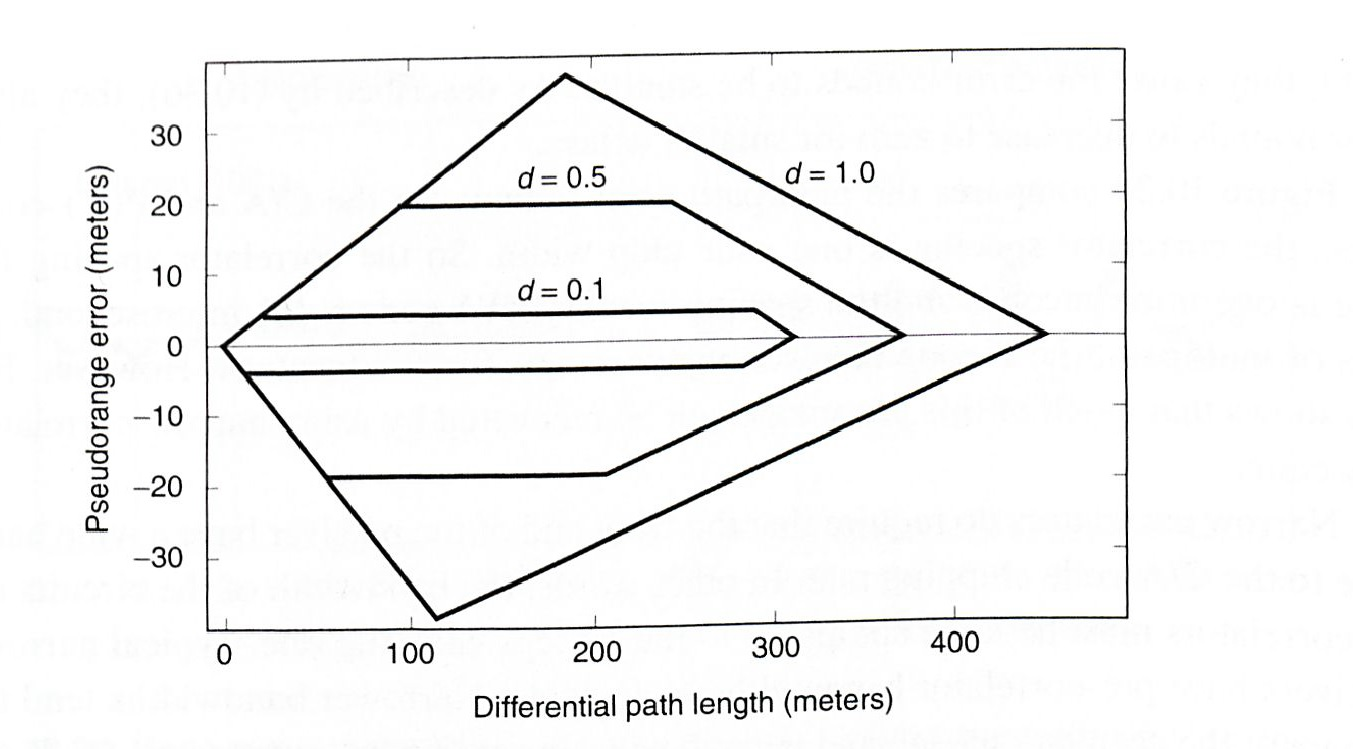
\includegraphics[scale=0.4,angle = -0.8]{images/Hullkurve}
	\caption{Mehrwege-Fehlerhüllkurve wie sie in GPS verwendet wird \cite{gps}}
	\label{fig:GPS Hüllkurve}
\end{figure}

Um die \gls{CRLB} für einen Mehrwegekanal zu berechnen, muss allerdings dessen statistisches Modell vorhanden sein. Für den Betragsgang der Übertragungsfunktion eines solchen Kanals gibt es Verteilungen, wie beispielsweise die Rayleigh-Verteilung. Diese ist allerdings nur für die Messung der Signalleistung relevant. Ist man jedoch an einer Messung der Phase interessiert, existiert bisweilen kein gutes Modell. In \cite{Lindner_CRLB} wurde die \gls{CRLB} für einen Zweipfadkanal berechnet. Bei der Arbeit geht es um Richtungsmessung, welche der Phasenmessung sehr ähnlich ist. Das Ergebnis zeigt allerdings, dass für starke Korrelation zwischen den beiden Pfaden, die \gls{CRLB} divergiert. Dies gilt sogar für hohe Dämpfungsfaktoren $\alpha$ des zweiten Pfades. Deshalb ist es nicht sinnvoll, dieses Maß für einen solchen Kanal zu verwenden. Die Schätzverfahren sollen mit einer Methode aus dem Forschungsbereich des \gls{GPS} evaluiert werden.
Bei \gls{GPS} wird die Signallaufzeit über Korrelation gemessen. Wenn der Umwegpfad kürzer als die Zeitdauer eines Samples ist, kann der Korrelator diesen nicht mehr auflösen. Diese Effekte werden mittels Fehlerhüllkurven, wie sie beispielhaft in Abbildung \ref{fig:GPS Hüllkurve} zu sehen sind, untersucht. Eine Mehrwege-Fehlerhüllkurve trägt den Laufzeitfehler über die Differenz aus Umwegpfad und LOS auf. Dabei lassen sich die Einflüsse der Länge des Umwegpfades, aber auch der Einfluss der Phasendrehung durch Reflektoren, gut veranschaulichen.
Zur Auswertung der Robustheit gegenüber Mehrwegeausbreitung sollen auch in dieser Arbeit Fehlerhüllkurven verwendet werden. 
 

\section{Signalcharakteristik}
\label{chap2.4:Signalcharakteristik}
Aus dem Kanalmodell und der Schätztheorie können einige Erkenntnisse darüber erlangt werden, wie ein Signal auszusehen hat, damit es trotz der Einflüsse des Kanals, robust gegenüber Mehrwegeausbreitung und schätzfehler-minimierend gegenüber dem \gls{AWGN}-Kanal ist. In diesem Kapitel sollen diese Eigenschaften zusammengetragen und Möglichkeiten zur Erzeugung solcher Signale vorgestellt werden. 


Da aus \eqref{eq:CRLB_Range} die Beziehung $\sigma_{range}^2 \sim \nicefrac[]{1}{\beta_{rms}^2}$ entnommen werden kann, ist es nötig die effektive Bandbreite zu maximieren. Ein Signal mit der Signalenergie an den Bandkanten würde diese Bedingung erfüllen. Allerdings ist aus dem Kanalmodell für Mehrwegeausbreitung ersichtlich geworden, dass ein Zweiton nicht besonders robust gegenüber destruktiver Interferenz ist. Dies offenbart ein Optimierungsproblem, bei welchem möglichst viel Energie an den Bandkanten, aber auch gleichzeitig auf dem Band verteilt werden muss, um gegenüber beiden Kanalmodellen robust zu sein. Deshalb sollen Mehrtonsignale mit unterschiedlichen Subträgerverteilungen untersucht werden, um herauszufinden wie diese auf den Kanal reagieren. 
Ausgehend von einem Zweiton, werden immer mehr Träger dem Band hinzugefügt. 

Zusätzlich muss der Energiebedarf beachtet werden. Signalerzeugung energiesparsam umzusetzen ist deshalb äußerst wichtig. Im Folgenden werden zwei Möglichkeiten gezeigt, wie solche Mehrtonsignale sparsam generiert werden können. 

\subsection{Hadamard-Sequenzen}
\label{chap2.4.1:Hadamard}
Hadamard-Sequenzen bieten die Möglichkeit das Band mit unterschiedlich vielen Trägern auszufüllen, je nachdem, welche Sequenz man auswählt. Die Sequenzen resultieren aus den Zeilen einer Hadamard-Matrix. Eine Hadamard-Matrix zeichnet sich dadurch aus, dass  Zeilen- und Spaltenvektoren jeweils zueinander orthogonal sind und die Einträge nur die Werte 1 und -1 annehmen können. Das Bildungsgesetz einer solchen Matrix ist ein rekursiver Algorithmus mit dem Anfangswert $H_{1x1} = 1$. Um daraus eine $2^{\nu}x\,2^{\nu}$ Matrix zu erzeugen gilt folgende Regel: 

\begin{equation}
	\label{eq:Hadamard-Matrix}
	H_{2^{\nu} x 2^{\nu}} = 
	\begin{pmatrix}
		H_{2^{\nu}} & \;\;\,H_{2^{\nu}} \\ H_{2^{\nu}} & - H_{2^{\nu}}
	\end{pmatrix}	 
\end{equation} 

Nicht alle Zeilen einer solchen Matrix spreizen das Spektrum. Die erste Zeile einer jeden Hadamard-Matrix besteht nur aus Einsen und hat daher nur einen Gleichanteil. Eine $H_{4x4}$-Matrix erzeugt vier Sequenzen. Die erste Sequenz schwingt nicht, die Zweite ist ein Einton und die Dritte und Vierte sind zwei Varianten desselben Zweitons. Für die Signalerzeugung von Mehrtonsignale werden erst Matrizen für $\nu \geq 3$ verwendet. In \eqref{eq:Hadamard-Matrix} ist eine $H_{8x8}$ beispielhaft ausgerechnet worden. 

\begin{equation}
	\label{eq:Hadamard8x8}
	H_{8 x 8} = \begin{pmatrix}
	1&1&1&1&1&1&1&1\\
	1&-1&1&-1&1&-1&1&-1\\
	1&1&-1&-1&1&1&-1&-1\\
	1&-1&-1&1&1&-1&-1&1\\
	1&1&1&1&-1&-1&-1&-1\\
	1&-1&1&-1&-1&1&-1&1\\
	1&1&-1&-1&-1&-1&1&1\\
	1&-1&-1&1&-1&1&1&-1
	\end{pmatrix}
\end{equation}

Diese Matrix liefert acht Sequenzen. In Abbildung \ref{fig:Hadamarspektren} wurde die \gls{DFT} von Signalen, bestehend aus Wiederholungen dieser Sequenzen berechnet. Die x-Achse der Abbildungen stellt eine normierte Frequenz dar, die y-Achse den normierten Betrag der \gls{DFT}. Die erste Sequenz hat ihre gesamte Energie bei der Frequenz Null. Die zweite Sequenz ist eine cosinusartige Schwingung, welche die gesamte Bandbreite ausnutzt. Des Weiteren sind die Sequenzen 3 und 4 Schwingungen, die nur die halbe Bandbreite ausnutzen. Die Sequenzen 5 und 7 bzw. 6 und 8 sind identisch. Wenn man die Sequenzen genauer betrachtet, sind sie verschobene Varianten voneinander. Eine $H_{8x8}$-Matrix liefert für unsere Zwecke somit drei Zweitöne und vier Viertöne. Um für spätere Auswertungen mehr Subträger einzufügen, werden $H_{16x16}$- und $H_{32x32}$-Matrizen verwendet. 

\begin{figure}[htbp]
	\centering
	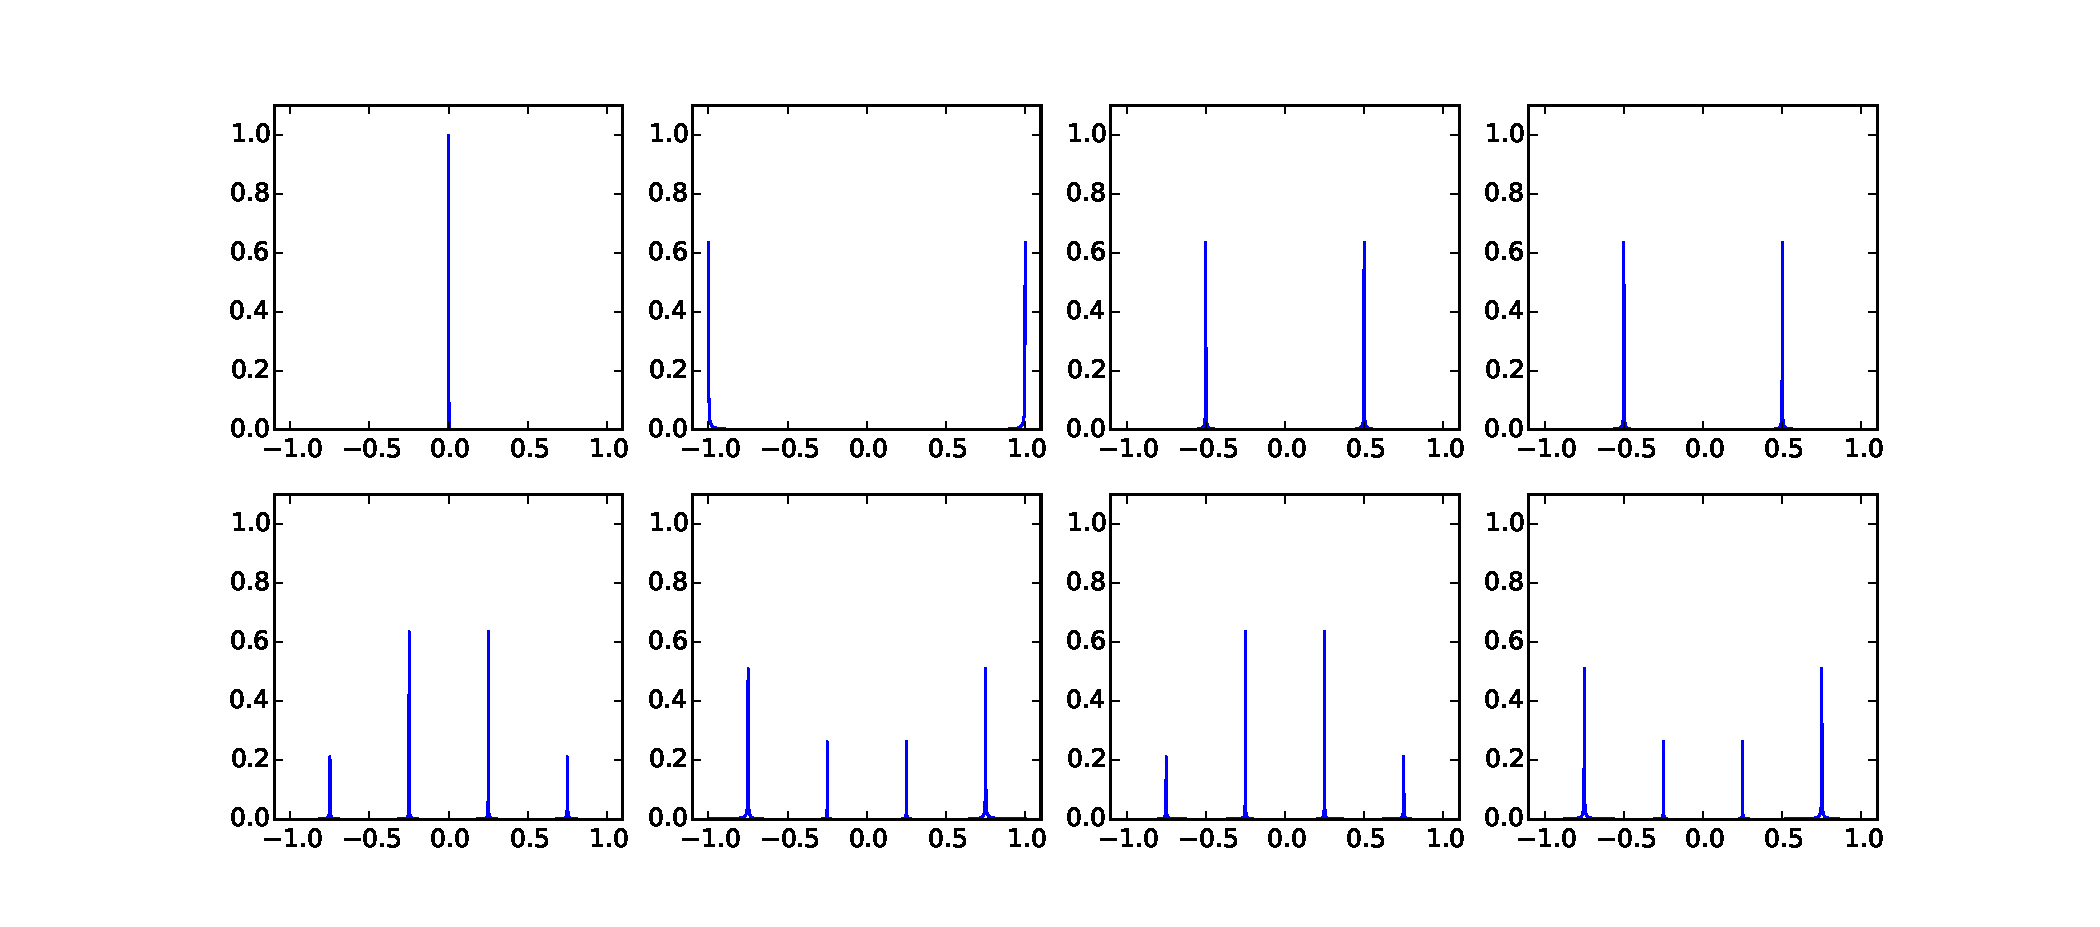
\includegraphics[width = \textwidth]{images/Hadamardspektren}
	\caption{DFT aller Hadamard-Sequenzen einer 8x8 Matrix}
	\label{fig:Hadamarspektren}
\end{figure}

Hadamard-Sequenzen können nur Spektren erzeugen, die eine gerade Anzahl an Subträgern haben und symmetrisch sind. 

\subsection{$m$-Sequenzen}
\label{chap2.4.2:m}
Eine weitere Methode zur spektralen Spreizung bieten \emph{maximal length linear shift} Register. Sie erzeugen die nach ihnen benannten $m$-Sequenzen. Eine solche Sequenz wird aus einem Schieberegister mit n Speicherzellen generiert. Die Anzahl der möglichen Zustände beträgt $2^n$. Der Zustand, bestehend aus ausschließlich Einsen, würde sich immer wieder selbst erzeugen. Ohne diesen Zustand nimmt ein Schieberegister mit $n$ Speicherzellen $2^n - 1$ Zustände ein, bevor sich die Sequenz wiederholt. Bei einem Register der Länge $n = 3$ erhält man eine Sequenz der Länge $2^3 - 1 = 7$. In Abbildung \ref{fig:Schieberegister} ist ein solches Schieberegister mit dem Anfangszustand <-1,1,1> abgebildet.  

\begin{figure}[htbp]
	\centering
	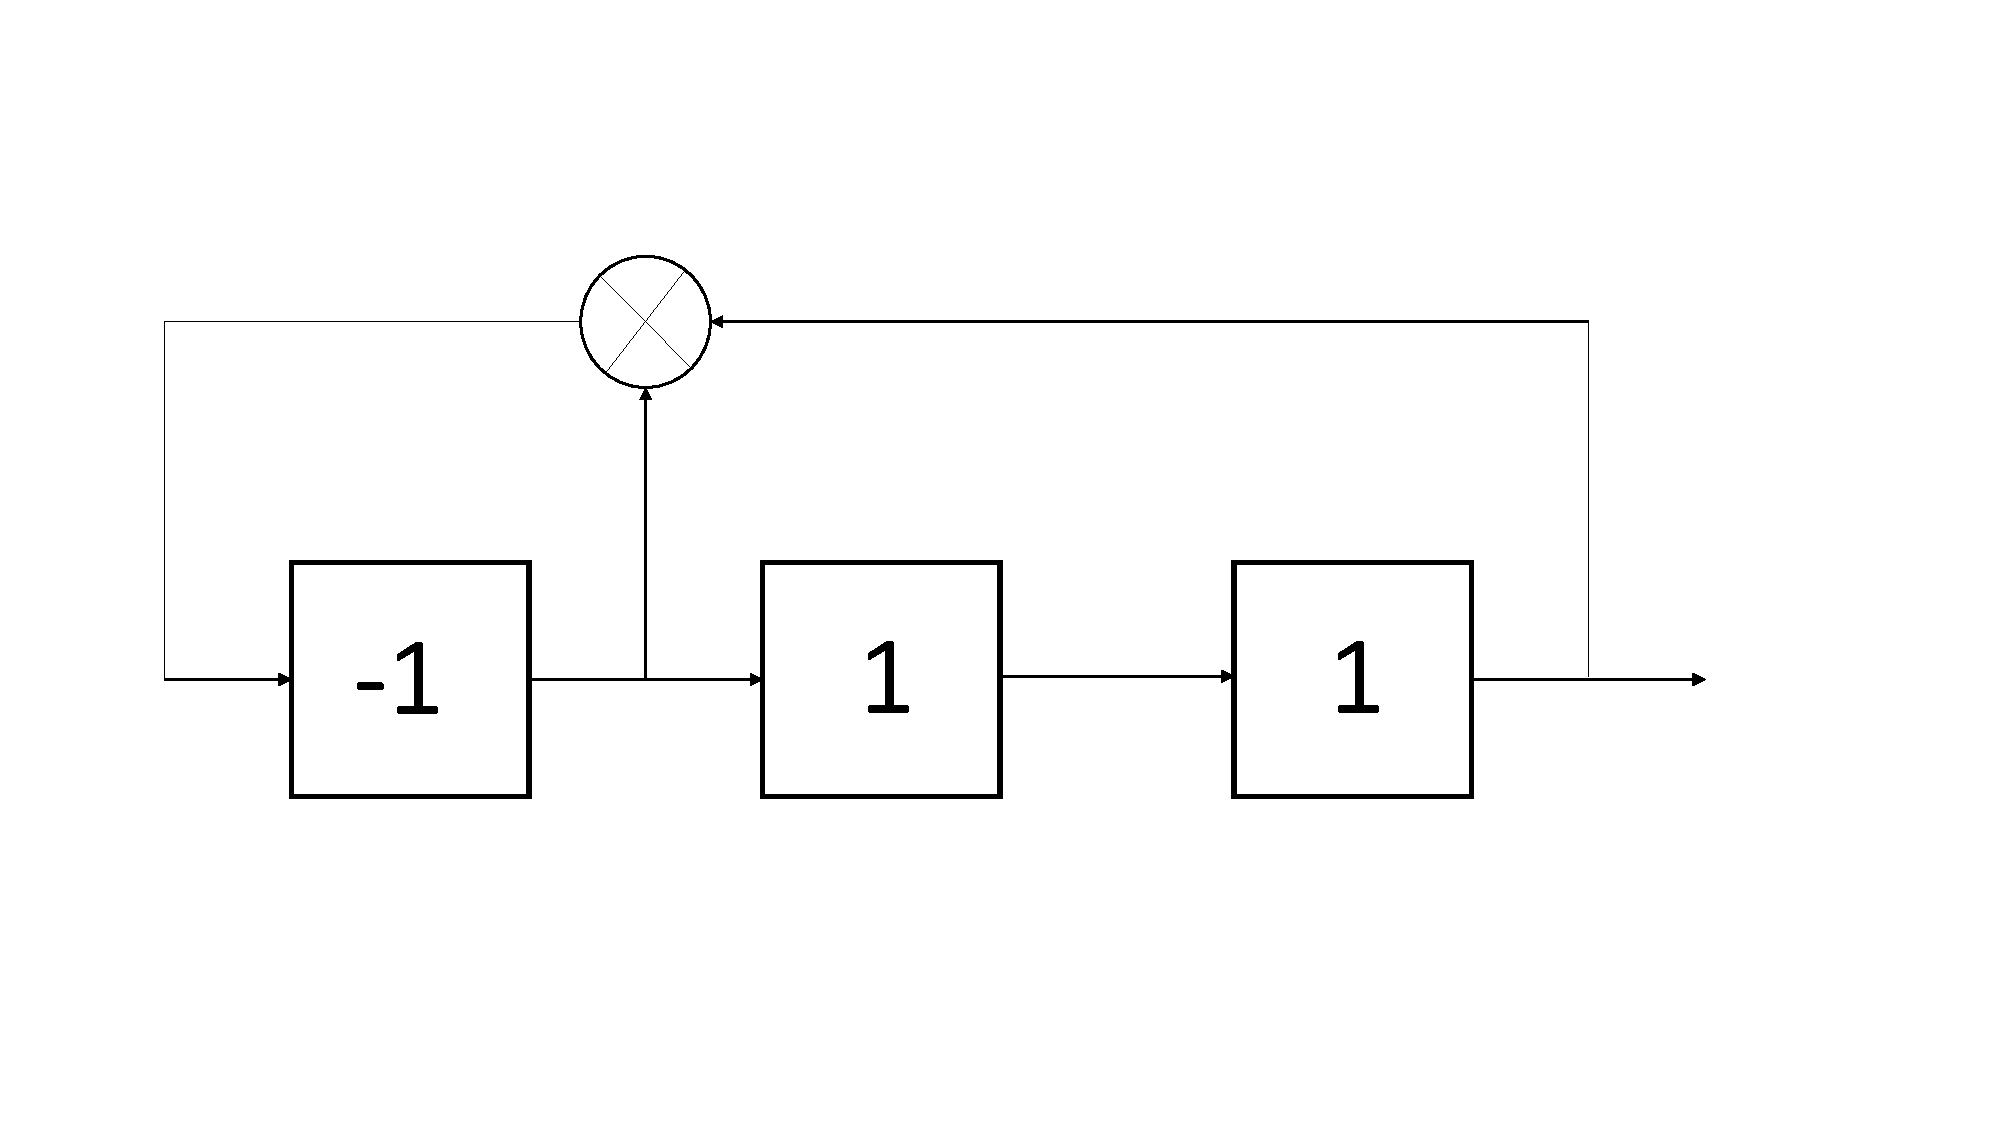
\includegraphics[width = 0.5\textwidth]{images/Schieberegister}
	\caption{Schieberegister mit Anfangszustand <-1,1,1>}
	\label{fig:Schieberegister}

\end{figure} 

Die Speicherzelle, nach der zurück gekoppelt wird, ist frei wählbar. Des Weiteren kann an mehreren Stellen zurück gekoppelt werden. Mit der Konfiguration des Registers in Abbildung \ref{fig:Schieberegister} würde demnach die Sequenz <1, 1, -1, 1, -1, -1, -1> entstehen. 
Jede $m$-Sequenz hat ein nahezu weißes Spektrum. Wird diese Sequenz periodisch wiederholt, entsteht ein Linienspektrum. Im Bereich der \gls{DFT} werden zwischen den diskreten Subträgern Nullen eingefügt. Damit entspricht die Anzahl der Subträger einer $m$-Sequenz, ihrer Länge.

\input{content/3-Schätzverfahren}
\chapter{Signalerzeugung und Kanalsimulation}
\label{chap:Signalerzeugung}

In diesem Kapitel sollen die in der Simulation verwendeten Signal-Parameter und -Erzeugung erläutert werden. Anschließend wird die Implementierung des Kanals kurz umrissen.

\section{Simulationsparameter}
\label{chap4.1:Simulationsparameter}
In Abschnitt \ref{chap2.4:Signalcharakteristik} wurde bereits erklärt, wie Mehrtonsignale erzeugt werden können. In diesem Abschnitt werden deren Parameter für die Simulation festgelegt. 

\begin{itemize}
\item Signaldauer $T \approx \unit[0.5]{ms} $ 
\item Trägerfrequenz $f_c = \unit[868]{MHz}$
\item Bandbreite B $\equiv$ Chiprate $f_{chip} = \unit[2]{MHz}$
\item Abtastfrequenz $f_{sampling} = \unit[4]{MHz}$
\end{itemize}

Die Signaldauer hängt bei der Simulation von der Bandbreite \gls{symb:B} und der Anzahl der Symbole im Signal ab. 
Es wurde $\unit[2]{MHz}$ als Bandbreite gewählt, da dies die Standard-Bandbreite im $\unit[868]{MHz}$-Band ist.   
Ein  Chip entspricht einem Symbol in der Sequenz. Wenn die Chiprate $f_{chip} = \unit[2]{MHz}$ sein soll, dann beträgt die Symboldauer eines Chips $\unit[0.5]{\mu s}$. Die Wellenlänge der Trägerfrequenz ist $\lambda = \frac{c_0}{f} = \unit[35]{cm}$. Damit passen $428,6$ Schwingungen in einen Chip. Um eine geeignete Abtastfrequenz zu finden, muss zunächst das Nyquist-Shannon-Abtasttheorem erfüllt sein.  
 
\begin{equation}
	 \label{eq:Abtasttheorem}
	 f_{sampling} \geq 2\cdot \gls{symb:B}
\end{equation}

Da die Bandbreite $\unit[2]{MHz}$ beträgt, muss \gls{symb:fc} mindestens $\unit[4]{MHz}$ sein. Die Auswirkungen der Bandvergrößerung werden im folgenden Kapitel genauer erläutert.

\section{Signalerzeugung}
\label{chap4.2:Signalerzeugung}
Für die Auswertung wurden fünf Subträgerverteilungen im gegebenen Band ausgewählt. Aus den Hadamard-Sequenzen wurde ein 4-Ton, 8-Ton und 16-Ton verwendet. Die Spektren dieser vier Sequenzen sehen wie folgt aus:

\begin{figure}[htbp]
	\centering
	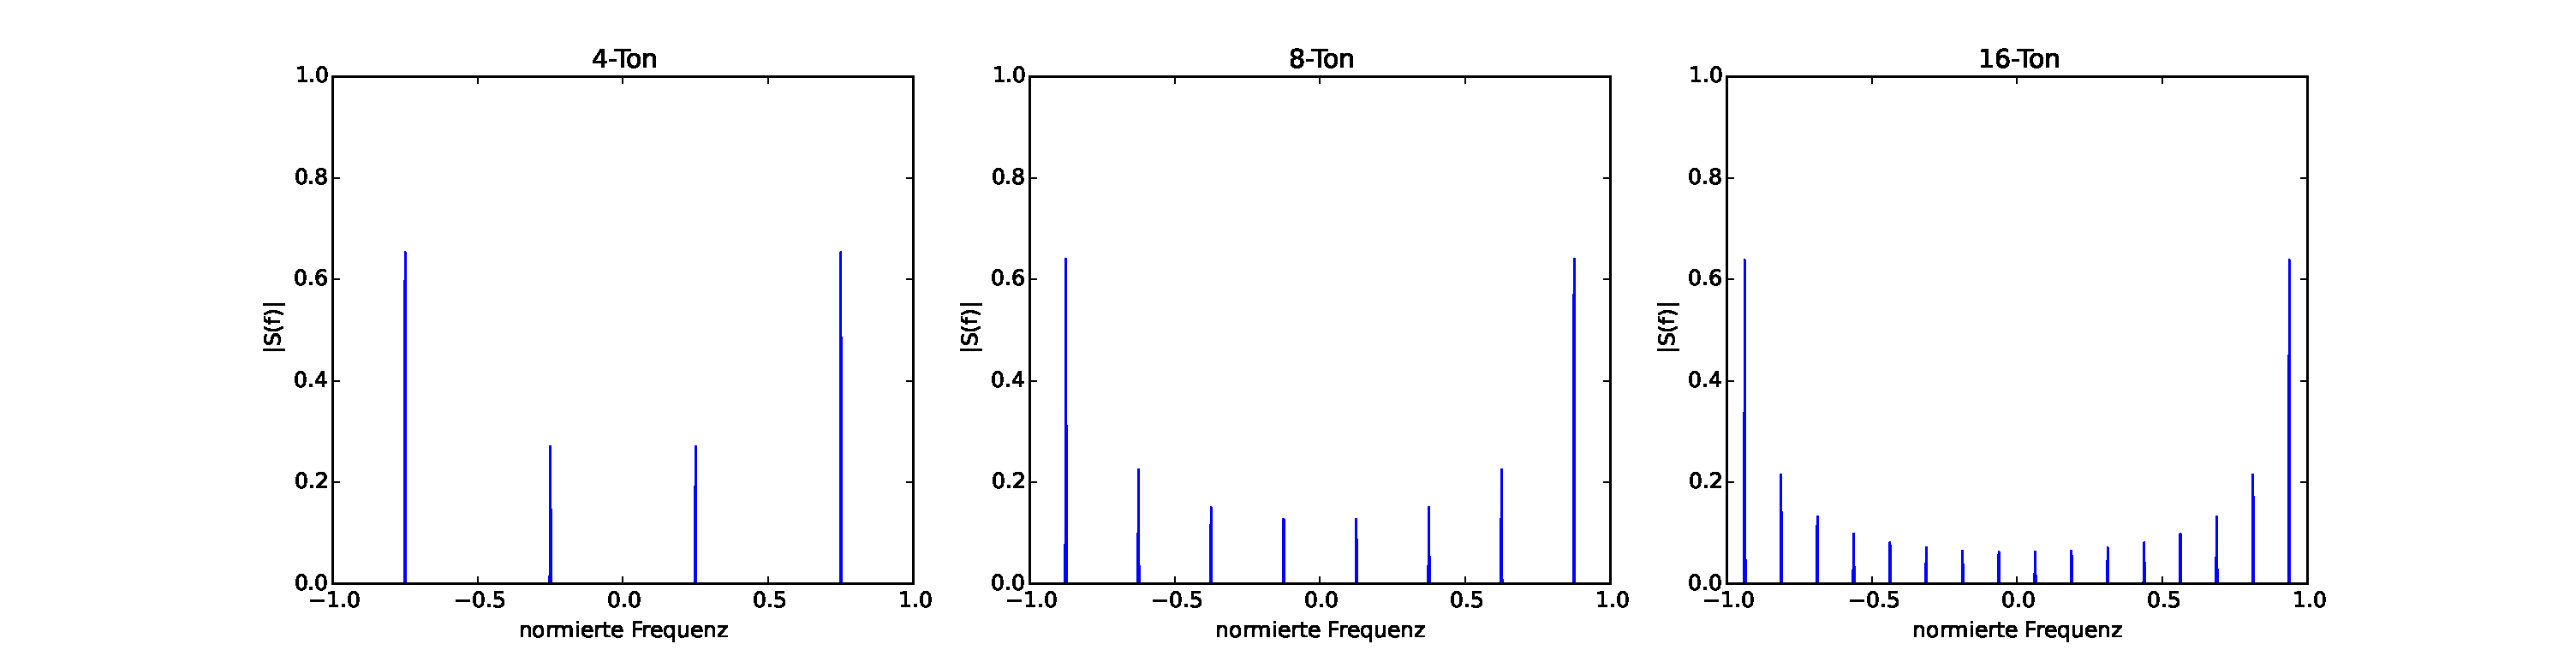
\includegraphics[width = \textwidth]{images/HadamardBeispiel}
	\caption{Normiertes Betragsspektrum der verwendeten Hadamard-Sequenzen}
	\label{fig:HadamardBeispiel}
\end{figure}
Es wurde darauf geachtet, dass die Subträger an den Bandkanten stärker gewichtet sind um die \gls{CRLB} der der Signale so klein wie möglich zu halten. Betrachtet man den 16-Ton, sieht er dem 8-Ton sehr ähnlich. Die äußeren beiden Subträger haben jedoch die gleiche Gewichtung wie der 8-Ton. Je mehr man in die Bandmitte geht, desto weniger stark sind die Subträger gewichtet.

Aus den $m$-Sequenzen wurde eine Sequenz der Länge 7 und eine der Länge 1023 gewählt. Dementsprechend viele Subträger haben sie.  
\begin{figure}[htbp]
	\centering
	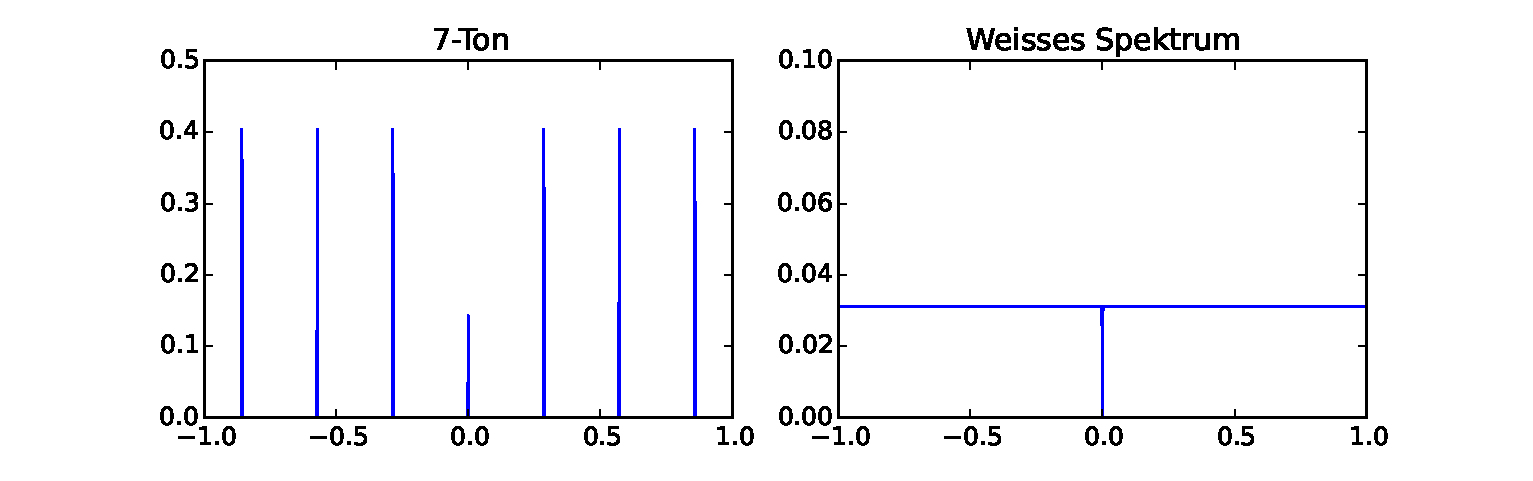
\includegraphics[width = \textwidth]{images/mSeqBeispiel}
	\caption{Normiertes Betragsspektrum der verwendeten $m$-Sequenzen}
	\label{fig:mSeqBeispiel}
\end{figure}
Die x-Achse entspricht wieder der normierten Frequenz und die y-Achse einem normierten Betragsspektrum. Auffällig ist, dass Beträge der Subträger bei $m$-Sequenzen wesentlich niedriger sind. Da nach dem Theorem von Parseval, die Summe über dem quadratischen Betragsspektrum, die Energie des Signals ergibt, zeigen die Spektren der $m$-Sequenzen, dass die Energie stärker verteilt ist.

Damit aus diesen Sequenzen Signale entstehen, muss eine Impulsformung stattfinden.
Als Modulationsimpuls wurde ein Rechteck verwendet. Da ein ideales Rechteck ein unendlich langes Spektrum besitzt, kann dieses als Modulationsimpuls nicht realisiert werden. Anstatt dessen, wird eine Näherung vorgenommen. Ein Rechteck, welches beispielsweise mit zwei diskreten Werten abgetastet wird, ist bandbegrenzt.  
Die Fouriertransformation eines Rechtecks ist eine Sinc-Funktion.
Deshalb folgt aus der Modulation mit einem Rechteckimpuls, eine Multiplikation des Spektrums mit einer Sinc-Funktion. Je höher dieses Rechteck abgetastet wird, desto breiter ist die Sinc-Funktion im Frequenzbereich. Da unsere Chiprate $f_{chip} = \unit[2]{MHz}$ beträgt, muss die Rate, mit der das Rechteck abgetastet wird, $\unit[4]{MHz}$ betragen, was auch der Breite der Sinc-Funktion entspricht. Aus einer diskreten Folge,  wird ein periodisches Spektrum erzeugt. Diese Periodizität ist in den Abbildungen \ref{fig:HadamardBeispiel} und \ref{fig:mSeqBeispiel} nicht zu erkennen, da die Abbildungen auf eine Periode bandbegrenzt sind. Das Spektrum des Rechtecks ist jedoch doppelt so breit wie in den vorherigen Abbildungen, deshalb werden die periodisch fortgesetzten Spektren mit dem Außenbereich der Hauptkeule der Sinc-Funktion gewichtet. Dieses Phänomen ist in Abbildung \ref{Modspek} verdeutlicht.

\begin{figure}[htbp] 
	\centering
	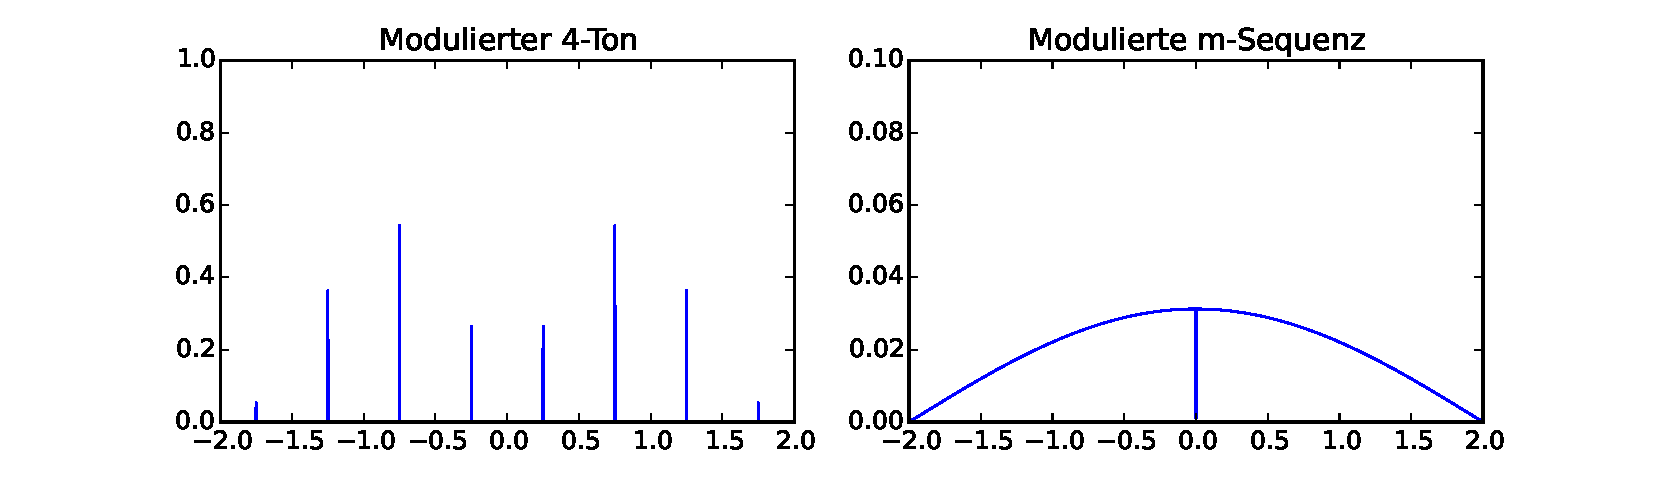
\includegraphics[width = \textwidth]{images/Modspek}
	\caption{Spektrum eines 4-Ton und einer $m$-Sequenz mit weißem Spektrum, moduliert mit einem Rechteck im Zeitbereich}
	\label{Modspek}
\end{figure}

Am Spektrum der modulierten m-Sequenz ist die Hauptkeule der Sinc-Funktion äußerst gut zu erkennen. Dieses Spektrum ist nun nicht mehr weiß. Am Spektrum des 4-Tons kann auch, außerhalb des $\unit[2]{MHz}$ Bandes, die gewichteten periodischen Wiederholungen beobachtet werden. Es befinden sich nun mehr Träger im Band, als gewollt. Deshalb muss nochmals bandbegrenzt werden. Auch nach der Bandbegrenzung ist ein kleiner Einfluss der Sinc-Funktion geblieben. Es muss beachtet werden, dass dieser Einfluss die effektive Bandbreite \gls{symb:brms} der Signale nach der Impulsformung verschlechtert hat, da die Subträger an den Bandkanten gestaucht werden. 

\section{Kanalsimulation}
\label{chap4.3:Kanalsimulation}

In Abschnitt \ref{chap2.2:Kanalmodell} wurden bereits die verwendeten Kanalmodelle vorgestellt. Jedes der verwendeten Modelle besteht aus einem Verzögerungsglied um die Laufzeit darzustellen. Die softwareseitige Realisierung einer Verzögerung der diskreten Folge ist allerdings von den Abtastwerten, \emph{Samples}, abhängig. Um die Folge zu verzögern, muss sie um n-Abtastwerte verschoben werden. Die kleinstmögliche Verzögerung die dabei bewerkstelligt werden kann, ist die um ein \emph{Sample}. Haben wir Beispielsweise eine Abtastrate von $ f_{sampling} = \unit[2]{MHz}$, dann sind zwei benachbarte Abtastwerte $\frac{1}{f_{sampling}} = \unit[0,5]{\mu s}$ bzw. $\unit[150]{m}$  voneinander entfernt. Dies ist allerdings zum Testen der Algorithmen nicht zielführend, da Mehrwegestörungen schon bei geringeren Distanzen auftreten. Deshalb muss eine Möglichkeit gefunden werden, einen Umwegpfad zu simulieren, der kürzer als $\unit[150]{m}$ ist. Um eine Verzögerung im Subsamplebereich zu realisieren, bietet es sich an, ein \emph{Fractional-Delay-Filter} zu verwenden. 

\subsection{Fractional-Delay-Filter (FD-Filter)}
\label{chap4.3.1:FD-Filter}
Um einen solchen Filter zu entwerfen, muss die Übertragungsfunktion einer Verzögerung in den Zeitbereich zurück transformiert werden. In Formel \ref{eq:Verschiebungssatz} sehen wir, dass die Übertragungsfunktion $H(e^{j\omega}) = e^{-j\omega D}$ ist, wobei $D$ den Verzögerungswert in Samples darstellt\cite{fd-filter}. $D$ kann in einen ganz- und gebrochenzahligen Anteil zerlegt werden. Die inverse Fouriertransformation dieser Übertragungsfunktion ergibt die, in \eqref{eq:Impulsresponse} zu sehende diskrete Impulsantwort. 

\begin{equation}
	\label{eq:Impulsresponse}
	h[n] = \frac{\sin(\pi(n-D))}{\pi(n-D)} = sinc[n-D]
\end{equation}

Die Impulsantwort muss mit dem Sendesignal gefaltet werden. Wenn $D$ ganzzahlig ist, geht die Funktion $sinc(n-D)$ in einen Dirac-Impuls bei $D$ über. Die Faltung ist folglich wie gewünscht eine Verschiebung um $D$. Wenn $D$ nicht ganzzahlig ist, wird die Sinc-Funktion um den ganzzahligen Anteil verschoben und versetzt abgetastet, was zu einer unendlichen Folge skalierter Dirac-Impulse führt. Das beantwortet die Frage, wo der verzögerte Signalwert liegt, da er sich nicht zwischen zwei Abtastwerten befinden kann. Im Idealfall sollte der Wert über das ganze Signal mit entsprechender Gewichtung verteilt werden. Gewichtet wird durch die Sinc-Funktion. In Abbildung \ref{fig:Sinc} wird dies beispielhaft für $D = 2$ und $D = 2.3$ dargestellt.

\begin{figure}[htbp]
	\centering
	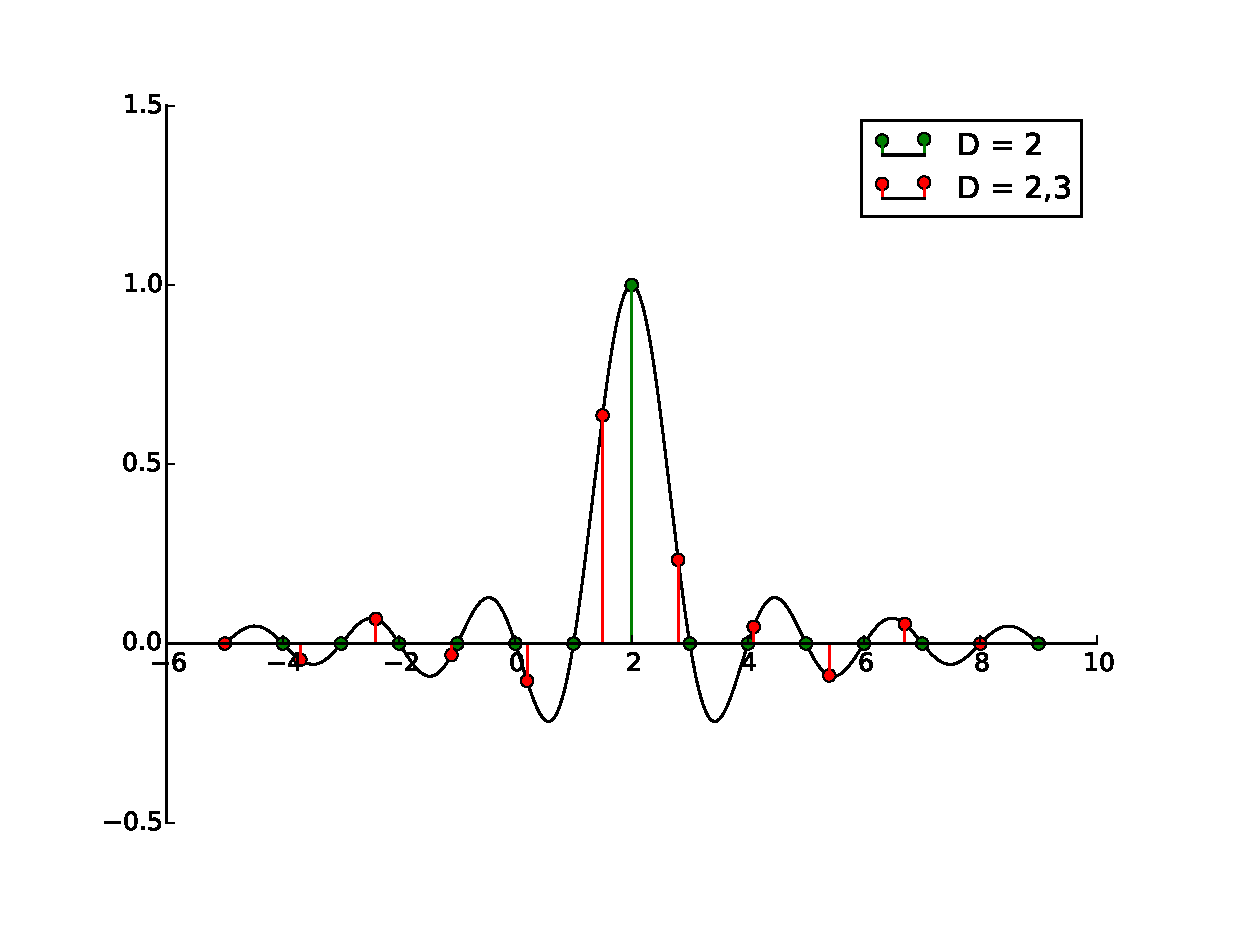
\includegraphics[scale=0.5]{images/Sinc}
	\caption{Impulsantwort eines Fractional Delay Filters}
	\label{fig:Sinc}
\end{figure}

Die ideale Impulsantwort ist, aufgrund ihrer Unendlichkeit, nicht realisierbar. Sie muss an irgendeinem Punkt abgeschnitten werden. Dies führt zu einem Ripple-Effekt im Frequenzbereich, welcher auch Gibb'sches Phänomen genannt wird. Dieser Effekt kann durch Wahl einer geeigneten Fensterfunktion minimiert werden.

\subsection{Implementierung}
Bei der konkreten Implementation wurde die Phase, mithilfe der Verzögerung, direkt im Frequenzbereich moduliert, und anschließend mit einer Rücktransformation die entsprechende Sinc-Funktion erzeugt. Da der Frequenzbereich der modulierten Exponentialfunktion auf das verwendetet Band begrenzt wurde, ist die Sinc-Funktion entsprechend gefenstert. In \cite{fd-filter} wurde dieses Fenster hergeleitet und sieht wie folgt aus:

\begin{equation}
	\label{eq:fd-window}
	w[n] = \frac{cos\left(\frac{\pi (n-D)}{N}\right)}{sinc\left(\frac{n-D}{N}\right)}  \;\;\; mit \;\;\; 0 \leq n \leq (N-1)
\end{equation}

Der Mehrwegekanal besteht aus Summation mehrerer gewichteter \gls{FD}, die mit einer zusätzlichen Exponentialfunktion multipliziert wurden, um die Reflektorphase zu berücksichtigen.  




 

\chapter{Auswertung}
\label{chap5:Auswertung}

In diesem Kapitel wird die Auswertung der im Rahmen dieser Arbeit erfolgten Simulationen vorgestellt und bewertet. 
Die Simulationsparameter wurden teilweise bereits in Abschnitt \ref{chap4.1:Simulationsparameter} beschrieben, sollen hier jedoch nochmal tabellarisch aufgeführt werden, \ref{tab:Simparmeter}. 

\begin{table}
	\centering	
	\begin{tabular}{ccc}
		\toprule
		
		Parameter & Symbol & Wert \\
		
		\midrule
		
		Trägerfrequenz & \gls{symb:fc} & $\unit[868]{MHz}$\\
		\\
		Bandbreite & \gls{symb:B} & $\unit[2]{MHz}$\\
		\\
		Abtastrate & $f_s$ & $\unit[4]{MHz}$\\
		\\
		Signaldauer & $T$ & $\unit[0.5]{ms}$\\
		\\
		Distanz & \gls{symb:r} & $\unit[150]{m}$ \\($\unit[1]{m}$- bzw. $\unit[15]{cm}$ Schritte)\\
		\\
		Sendesignalleistung & \gls{symb:PTx} & $\unit[10]{mW}$\\
		\\
		Rauschzahl des Empfängers & $NF$ & $\unit[8]{dB}$\\
				
		\bottomrule	
			
	\end{tabular}
	\caption{Simulationsparameter}
	\label{tab:Simparmeter}
\end{table}
Es wird zunächst eine Auswertung aller Schätzer im \gls{AWGN}- und anschließend im Mehrwegefall durchgeführt. Aus den Schlüssen dieser Betrachtungen sollen Schätzer und Signale mit der besten Leistung ausgewählt werden, um abschließend eine Auswertung unter Berücksichtigung des gesamten Kanalmodells durchzuführen. 
Im \gls{AWGN}-Fall wird der Schätzfehler über ein normiertes \gls{SNR} aufgetragen. Der normierte Wert, stellt die Signalleistung $P$ ins Verhältnis zur Rauschleistungsdichte $N_0$. Damit das \gls{SNR} bandbreitenunabhängig ist, wird die Signalleistung unter Berücksichtigung der verwendeten Bandbreite \gls{symb:B} in eine Signalleistungsdichte $C$ umgerechnet. 
Auf der x-Achse ist anstelle des \gls{SNR}, somit das Verhältnis \nicefrac[]{\gls{symb:C}}{\gls{symb:N0}} in $\unit[]{dB-Hz}$ dargestellt.
Wie in Abschnitt \ref{chap2.3:Schätztheorie} erläutert, soll der Schätzfehler im \gls{AWGN}-Fall mit der \gls{CRLB} verglichen werden. Dazu wird der \gls{rms}-Wert dieses Fehlers (\gls{rmse}) wie folgt berechnet:
\begin{equation}
	\label{eq:rmse}
	rmse(\hat{\tau}) = \sqrt{\overline{(\hat{\tau}-\tau)^2}}
\end{equation}

Aus diesem Wert und der \gls{CRLB} kann daraufhin die Schätzeffizienz $e$ nach \eqref{eq:e} angegeben werden, welche Schätzer- und Signalübergreifend verglichen werden kann. 

\begin{equation}
	\label{eq:e}
	e = \frac{\gls{CRLB}}{\gls{rmse}}
\end{equation}


Für Mehrwegeausbreitung werden die aus Abschnitt \ref{chap2.3.3:Hüllkurven} erläuterten Mehrwegehüllkurven verwendet, um den Fehler der Schätzer zu visualisieren. 
Für die abschließende Auswertung wird der \gls{rmse} über dem Gesamtkanal betrachtet. 


\section{Betrachtung für \gls{AWGN}-Fall}
\label{chap5.1:AWGN-Fall}
Um \gls{rmse} der Schätzverfahren bewerten zu können, soll er mit der \gls{CRLB}, für den betrachteten Kanal, verglichen werden. Die untere Schranke ist vom \nicefrac[]{\gls{symb:C}}{\gls{symb:N0}} und der effektiven Bandbreite \gls{symb:brms}, bzw. der Signalform abhängig. Das \nicefrac[]{\gls{symb:C}}{\gls{symb:N0}} wird von den Systemparametern und dem Kanal beeinflusst. In \cite{nowak2014system} wurde bereits eine Rauschbetrachtung für den Kanal, wie er im \glslink{BATS}{BATS}-Projekt vorliegt, durchgeführt. Bei einer gegebenen Sendeleistung \gls{symb:PTx} und Kenntnis über das Rauschverhalten des Empfängers, kann das \nicefrac[]{\gls{symb:C}}{\gls{symb:N0}} über die Streckendämpfung für beliebige Distanzen \gls{symb:r} berechnet werden. Da der natürliche Lebensraum, der im Rahmen des \glslink{BATS}{BATS}-Projektes untersuchten Fledermäuße, ein dichtes Waldgebiet ist, kann nicht von Freiraumausbreitung ausgegangen werden, um die Streckendämpfung zu berechnen. Es wird ein zusätzlicher Faktor benötigt, um Abschattungen und Dämpfungen der Signale durch Vegetation zu berücksichtigen. Bei einer Trägerfrequenz $f_c = \unit[868]{MHz}$ beträgt dieser Faktor $FC_1 = 0.25\cdot r$ \cite{nowak2014system}. Somit errechnet sich die Empfangsleistung zu:

\begin{equation}
	\label{eq:Prx}
	P_{rx,dB}(r) = P_{tx,dB} - 20log\left(\frac{4 \pi r f_c}{c_0}\right)- r\cdot FC_1
\end{equation}

Die Rauschleistung ergibt sich aus der Leistung des thermischen Rauschens und der Rauschzahl $NF = \unit[8]{dB}$ des Empfängers.
Das thermische Rauschen ist von der Boltzmann-Konstante $k_B = \unit[1.38\cdot 10^{23}]{Ws/K}$, der Temperatur $T = \unit[290]{K}$ und der Bandbreite \gls{symb:B} abhängig.  

\begin{equation}
	\label{eq:SNR}
	\left(\frac{C}{N_0}\right)_{dB}(r)=P_{rx,dB}(r)-N_{dB}-NF+B_{dB} 	
\end{equation}

mit 

\begin{equation}
	\label{eq:ThermRauschen}
	N = k_B\cdot T\cdot B
\end{equation}
Abschließend wird mit der Bandbreite \gls{symb:B} normiert. 
Das \nicefrac[]{\gls{symb:C}}{\gls{symb:N0}} nimmt aufgrund der immer kleiner werdenden Signalleistung über der Distanz ab. Diese Distanzabhängigkeit ist in Abbildung \ref{fig:SNR_Distanz und CRLB}(a) veranschaulicht.

\begin{figure}[htbp]
	\centering
	\makebox[\textwidth][c]{\begin{tabular}{ccc}
		\subfloat[\nicefrac{\gls{symb:C}}{\gls{symb:N0}}]{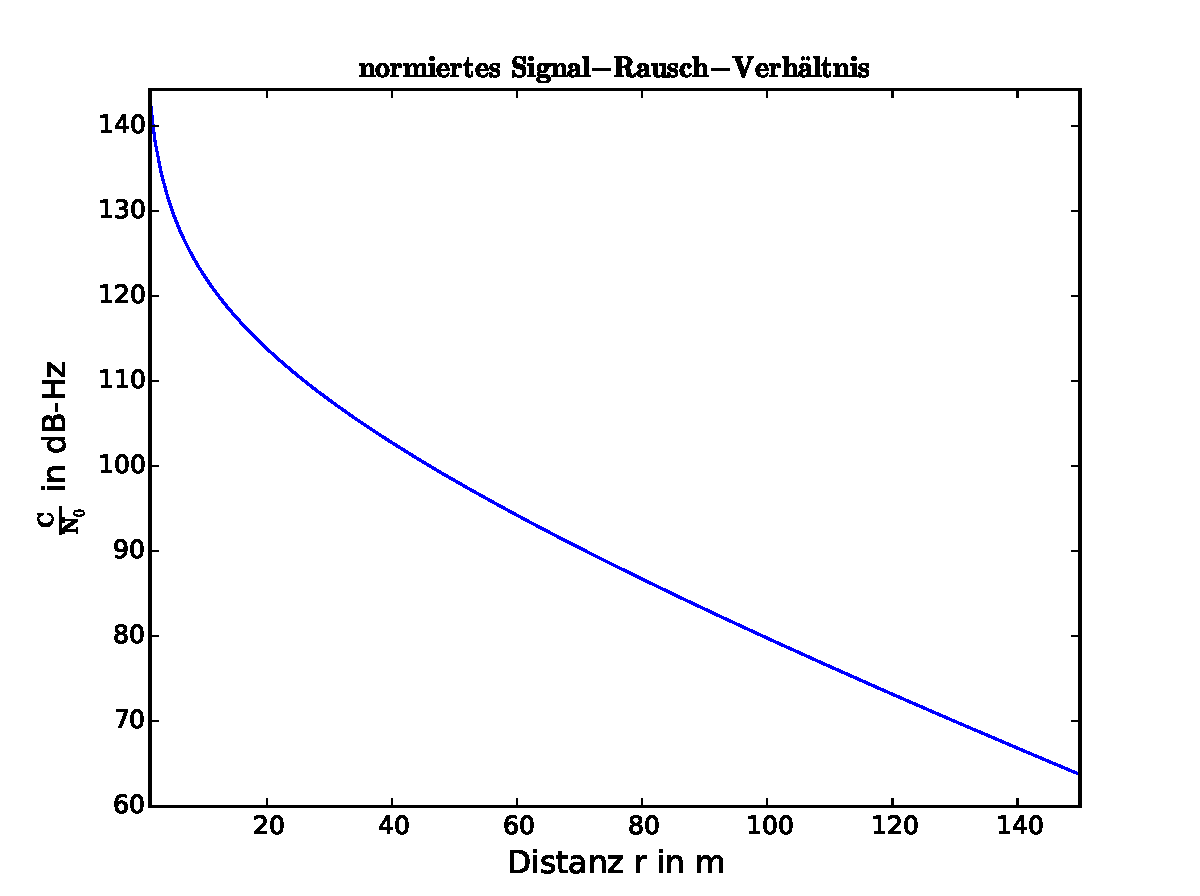
\includegraphics[width = 0.5\textwidth]{images/SNR_Distanz}} &
		\subfloat[\gls{CRLB}]{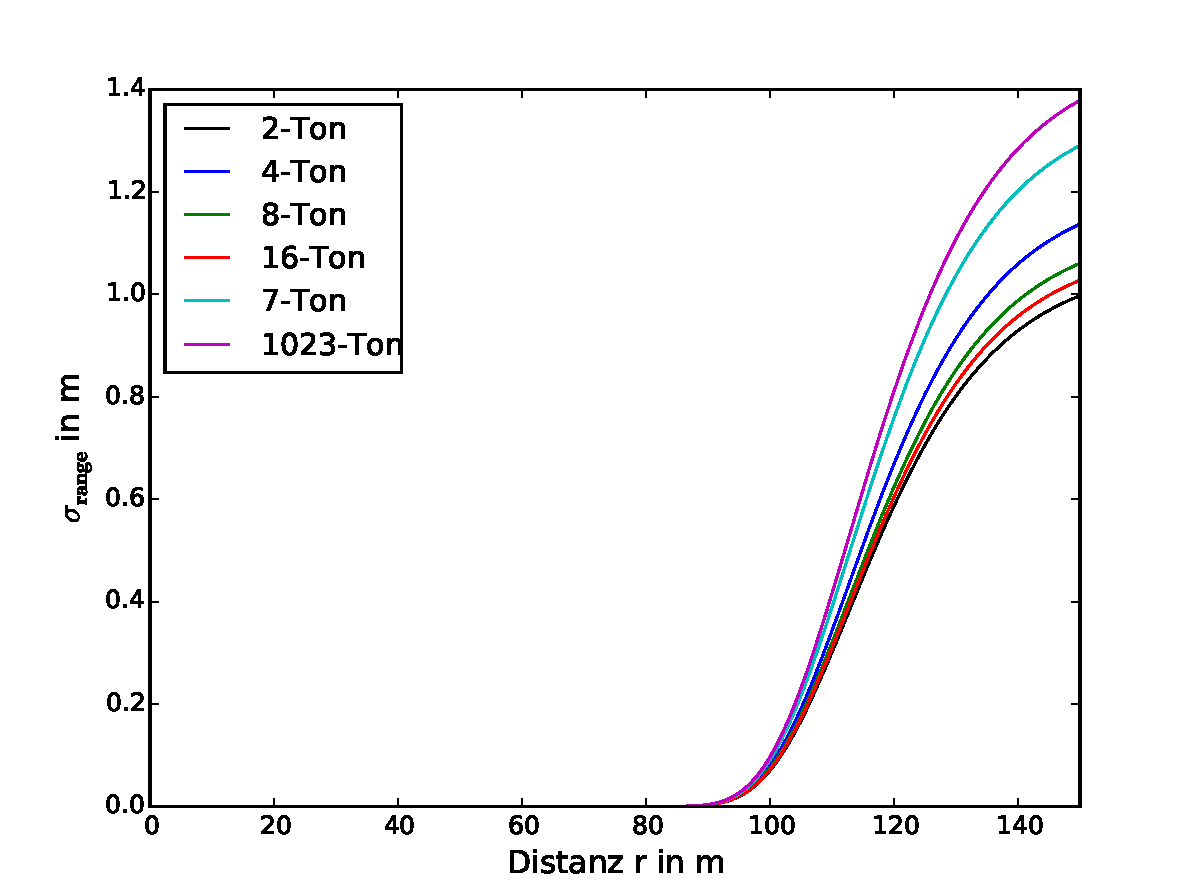
\includegraphics[width = 0.5\textwidth]{images/CRLB_Distanz}}	
	\end{tabular}}
	\caption{Distanzabhängige Auswirkung des \gls{AWGN}-Kanals auf das \nicefrac{\gls{symb:C}}{\gls{symb:N0}} und \gls{CRLB}}
	\label{fig:SNR_Distanz und CRLB}
\end{figure}

Mit kleiner werdenden \nicefrac[]{\gls{symb:C}}{\gls{symb:N0}}, wird die \gls{CRLB} nach \eqref{eq:CRLB_Range} größer. Aus diesem Grund weist sie ebenfalls eine Distanzabhängigkeit auf. Mit diesen Parametern ist es nun möglich die \gls{CRLB} nach \eqref{eq:CRLB_Range} für die Signale mit unterschiedlichem \gls{symb:brms} zu berechnen. Diese sind in \ref{fig:SNR_Distanz und CRLB}(b) abgebildet.
Der Abbildung \ref{fig:SNR_Distanz und CRLB}(a) ist des Weiteren zu entnehmen, dass bei einer Distanz von $\unit[150]{m}$ das \nicefrac[]{\gls{symb:C}}{\gls{symb:N0}}, Werte von $\unit[66]{dB-Hz}$ bis $\unit[140]{dB-Hz}$ annimmt. Anstatt die Auswertungen im Folgenden über die Distanz aufzutragen, werden sie über diesen Bereich des \nicefrac[]{\gls{symb:C}}{\gls{symb:N0}} veranschaulicht. In Abbildung \ref{fig:CRLB_SNR} ist die \gls{CRLB} der unterschiedlichen Signale im genannten Bereich des \nicefrac{\gls{symb:C}}{\gls{symb:N0}} abgebildet. Diese Kurven werden bei späteren Vergleichen als Referenz verwendet.
\begin{figure}[htbp]
	\centering
	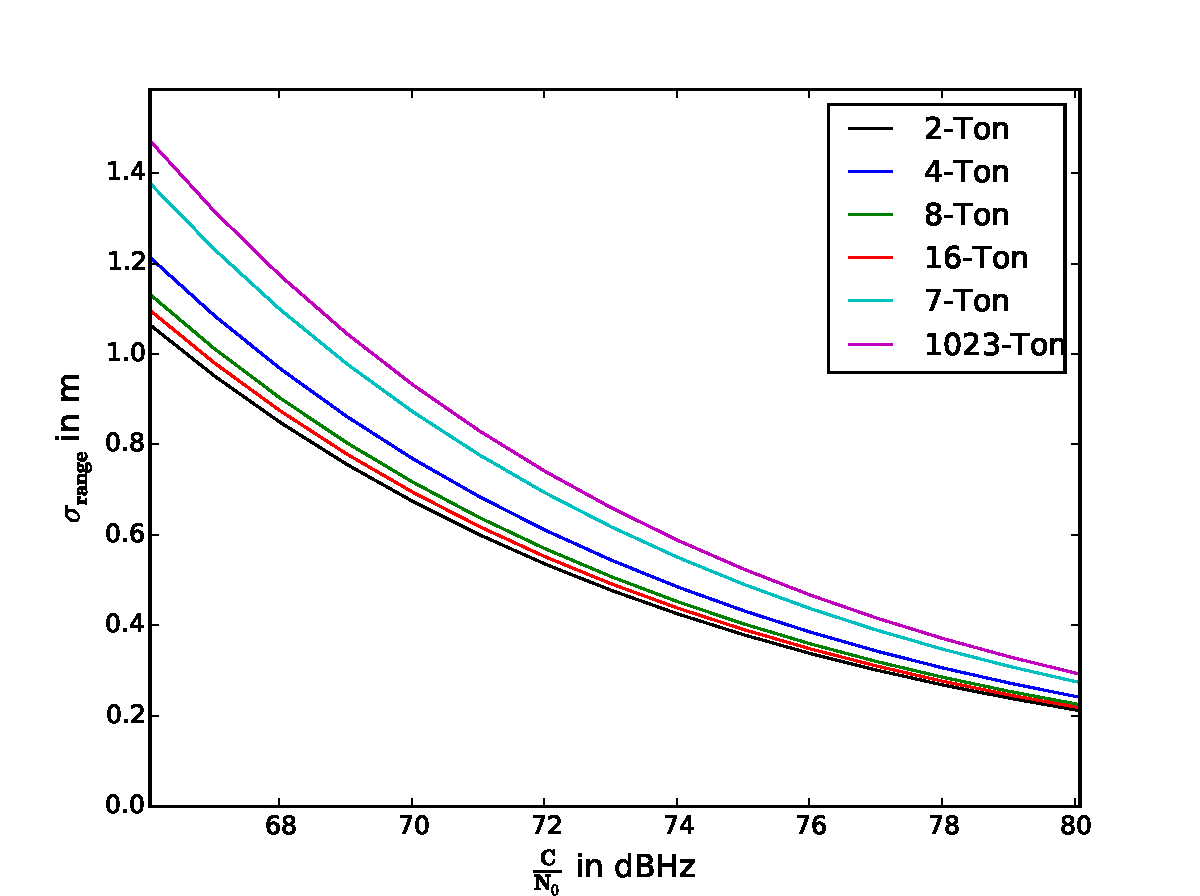
\includegraphics[width = 0.7\textwidth]{images/CRLB_Signale}
	\caption{\gls{CRLB} abhängig von \nicefrac[]{\gls{symb:C}}{\gls{symb:N0}}}
	\label{fig:CRLB_SNR}
\end{figure}
Lässt man alle anderen Parameter konstant, ist der 2-Ton das Signal mit der besten \gls{CRLB}. Ausgehend von diesem Signal sollte, bei weiterer Distribution der Energie, die Schranke größer werden. Dies wird in Abbildung \ref{fig:CRLB_SNR} bestätigt. Um wie viel sich die Schranke verschlechtert, ist von der Verteilung der Energie abhängig.
Je mehr Energie in Bandkantennähe ist, desto kleiner wird die Schranke. Die hier verwendeten Hadamard-Sequenzen haben die Eigenschaft, dass bei steigender Subträgerzahl, die stark gewichteten Subträger näher an die Bandkanten rücken. Damit liegt die Schranke des 16-Tons am nächsten an der des 2-Tons. 
Die $m$-Sequenzen sind nicht von diesem Effekt betroffen, da sie die Signalenergie immer auf alle Subträger gleich verteilen. Dadurch sind auch bei niedrigen Frequenzen, Subträger stark gewichtet, was folglich die \gls{CRLB} verschlechtert.


\subsection{Auswertung des gemittelten-Phasendifferenz-Schätzers}
\label{chap5.1.1:gemittelter Phasendifferenz Schätzer}
In diesem Abschnitt wird das Verhalten des gemittelten-Phasendifferenz-Schätzers, unter dem Einfluss des \gls{AWGN}-Kanals, untersucht. Es sollen Unterschiede, bei Verwendung der jeweiligen Testsignale, beobachtet und erläutert werden. 

\begin{figure}[htbp]
	\centering
	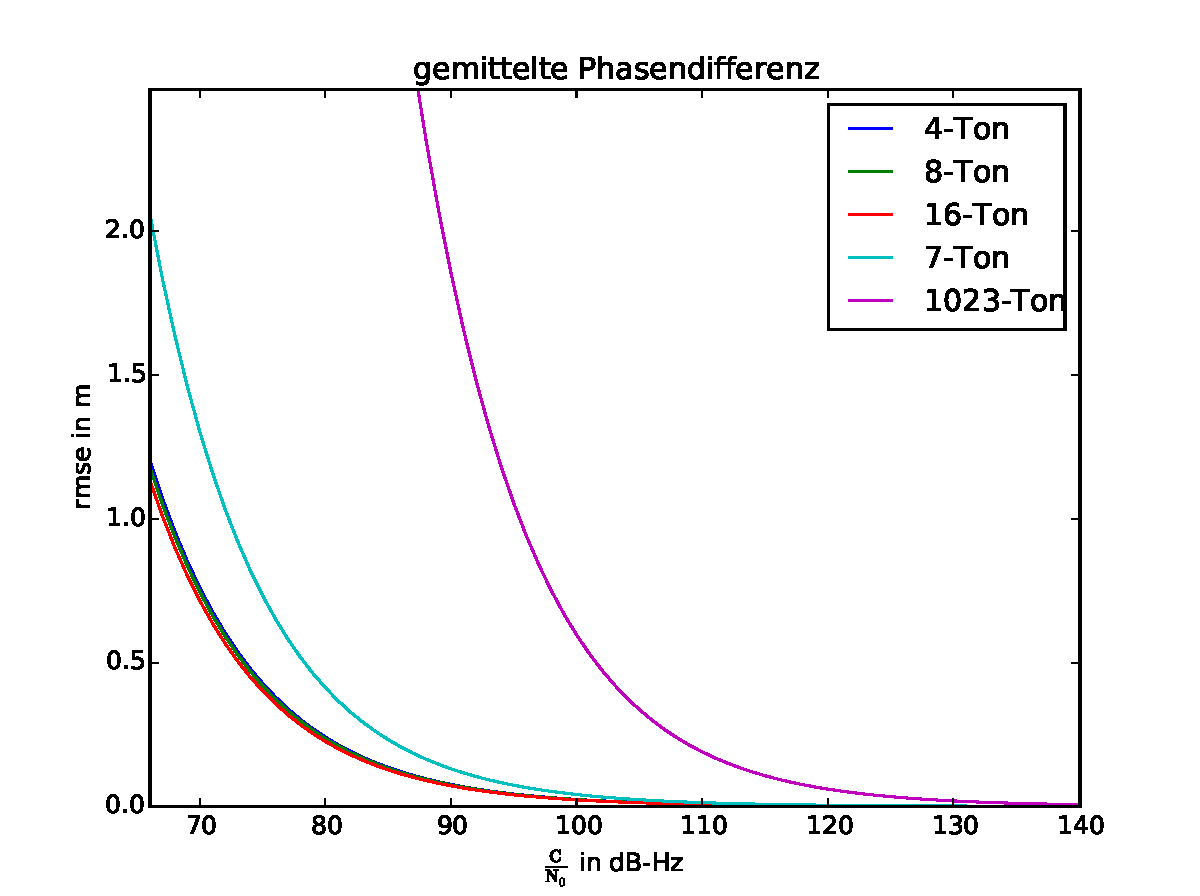
\includegraphics[width = 0.7\textwidth]{images/GemitteltePhasendiff_varianz}
	\caption{Simulation des Schätzfehlers der gemittelten Phasendifferenzschätzung bei einem \gls{AWGN}-Kanal}
	\label{fig:gemitteltePhasendiff_varianz}
\end{figure}

In Abbildung \ref{fig:gemitteltePhasendiff_varianz} ist zu sehen, dass die $m$-Sequenz mit 1023 Trägern stark von den restlichen Kurven abweicht. Grundsätzlich schneiden die $m$-Sequenzen im Vergleich zu den Hadamard-Sequenzen schlechter ab. Jedoch folgt dies, wie bereits erläutert, zwangsläufig aus der \gls{CRLB}.  
Um das Schätzverfahren unabhängig von der Signalcharakteristik zu evaluieren, wird der \gls{rmse} der einzelnen Signale mit der jeweiligen \gls{CRLB} aus Abbildung \ref{fig:CRLB_SNR} verglichen.

\begin{figure}[htbp]
	\centering
	\makebox[\textwidth][c]{\begin{tabular}{ccc}
			\subfloat[7-Ton]{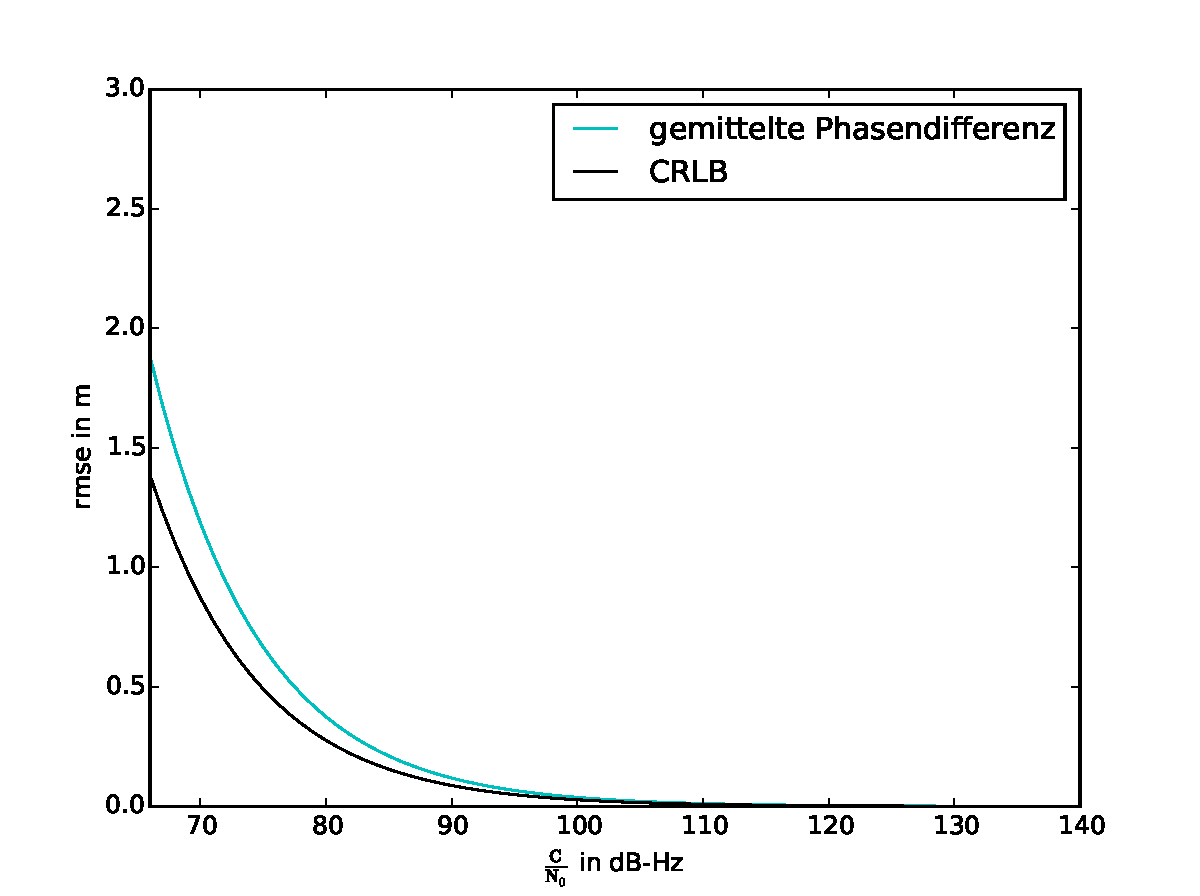
\includegraphics[width = 0.5\textwidth]{images/7-Ton_gegen_CRLB}} &
			\subfloat[1023-Ton]{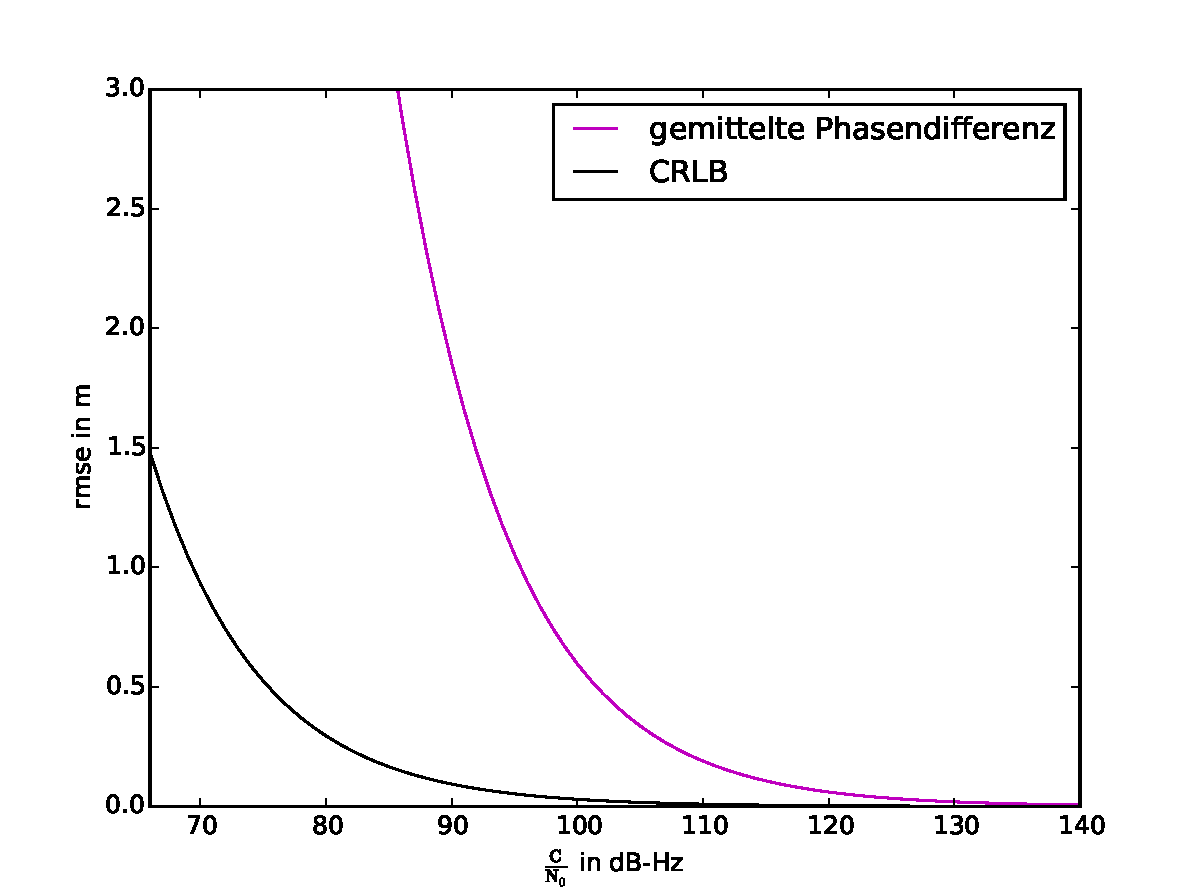
\includegraphics[width = 0.5\textwidth]{images/1023-Ton_gegen_CRLB}}
	\end{tabular}}
	\caption{\gls{rmse} der $m$-Sequenzen gegenüber der \gls{CRLB}}
	\label{fig:m_Phasendifferenz_CRLB_vergleich}
\end{figure}

Aus der Abbildung \ref{fig:m_Phasendifferenz_CRLB_vergleich} kann entnommen werden, dass dieses Schätzverfahren, bei Verwendung der $m$-Sequenzen, die untere Schranke nicht erreicht. Das ist bei den Hadamard-Sequenzen nicht der Fall.

\begin{figure}[htbp]
	\centering
	\makebox[\textwidth][c]{\begin{tabular}{ccc}	
		\subfloat[4-Ton]{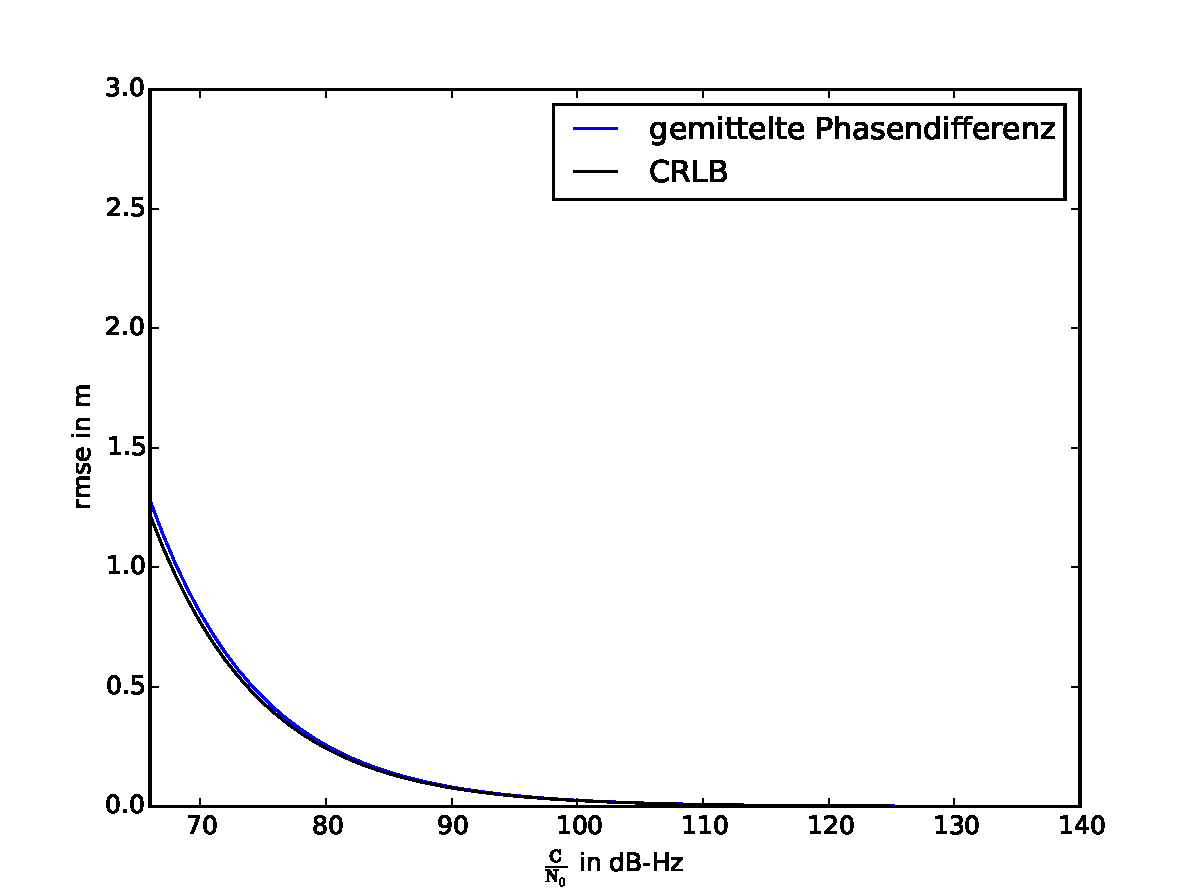
\includegraphics[width = 0.5\textwidth]{images/4-Ton_gegen_CRLB}}&
		\subfloat[8-Ton]{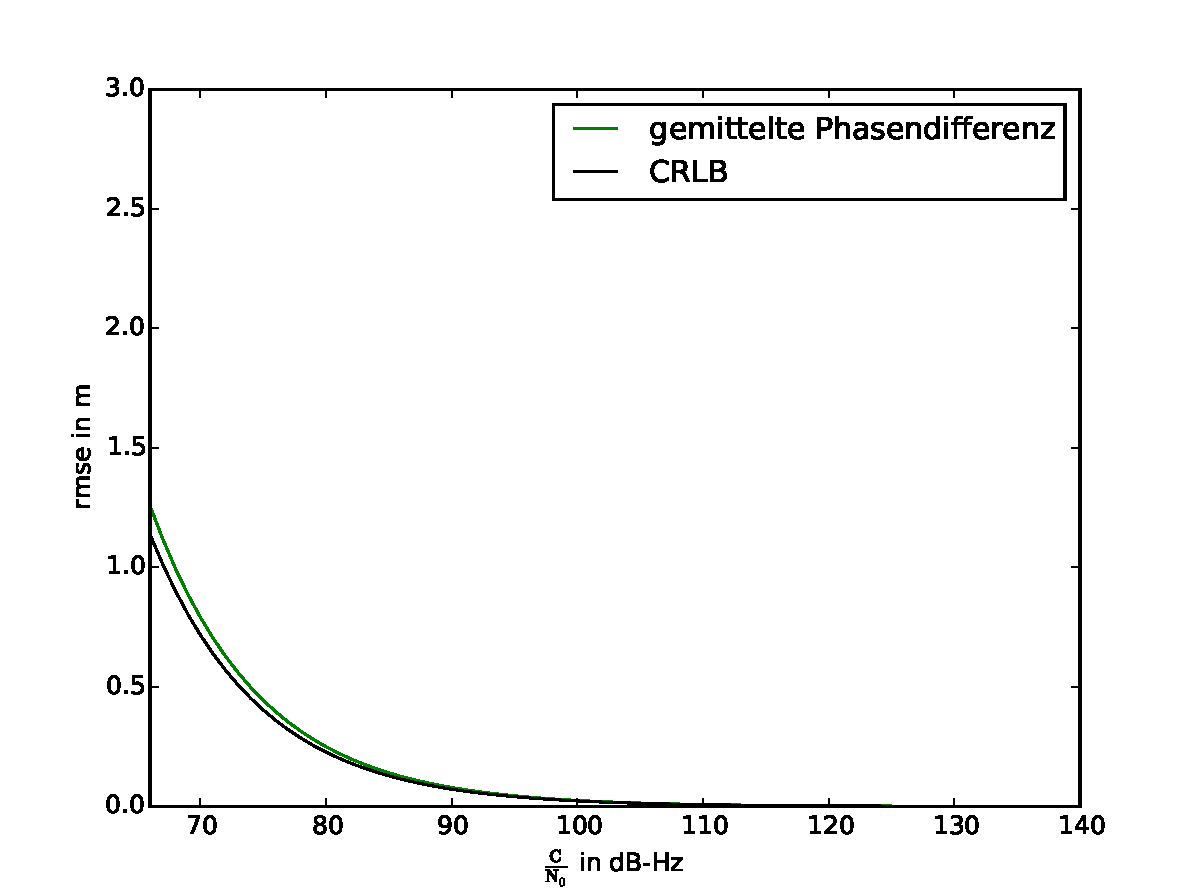
\includegraphics[width = 0.5\textwidth]{images/8-Ton_gegen_CRLB}}
		\end{tabular}}
	\makebox[\textwidth][c]{\begin{tabular}{ccc}
		\subfloat[16-Ton]{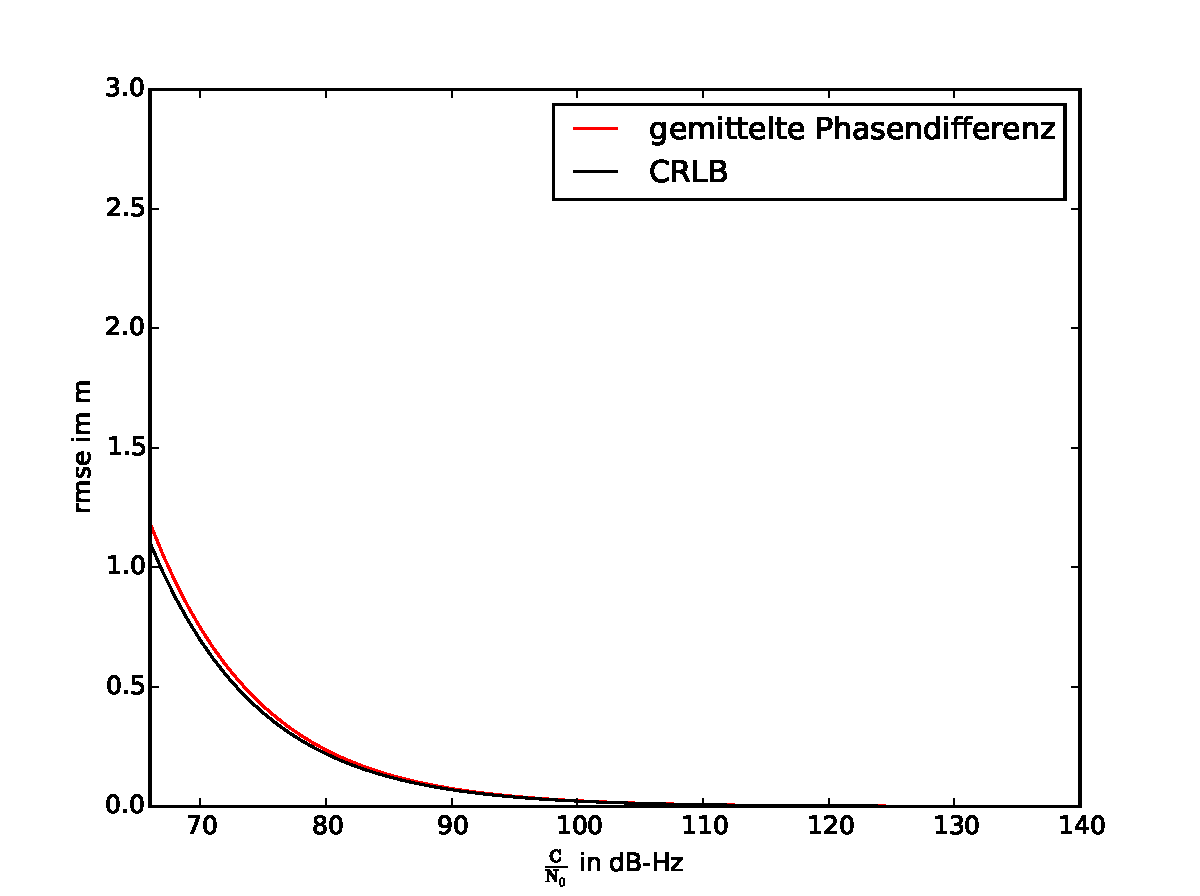
\includegraphics[width = 0.5\textwidth]{images/16-Ton_gegen_CRLB}}\\
	\end{tabular}}		
	\caption{\gls{rmse} der Hadamard-Sequenzen gegenüber der \gls{CRLB}}
	\label{fig:Had_Phasendifferenz_CRLB_vergleich}	
\end{figure}		
		
In Abbildung \ref{fig:Had_Phasendifferenz_CRLB_vergleich} ist zu sehen, dass für diese Signalformen dieser Schätzer die \gls{CRLB} nahezu für alle drei Testsignale erreicht. Welche Signalform am nächsten an der \gls{CRLB} liegt, kann aus Abbildung \ref{fig:m_Phasendifferenz_CRLB_vergleich} und \ref{fig:Had_Phasendifferenz_CRLB_vergleich} nicht klar abgelesen werden. Um eindeutig bestimmen zu können, welche Signalform die beste Leistung mit den hier verwendeten Schätzverfahren erzielt, muss die Schätzeffizienz nach \eqref{eq:e} betrachtet werden. Sie nimmt Werte zwischen 0 und 1 an, wobei die maximale Schätzeffizienz erreicht ist, wenn die Varianz des Schätzfehlers auf der \gls{CRLB} liegt. 

\begin{figure}[htbp]
	\centering
	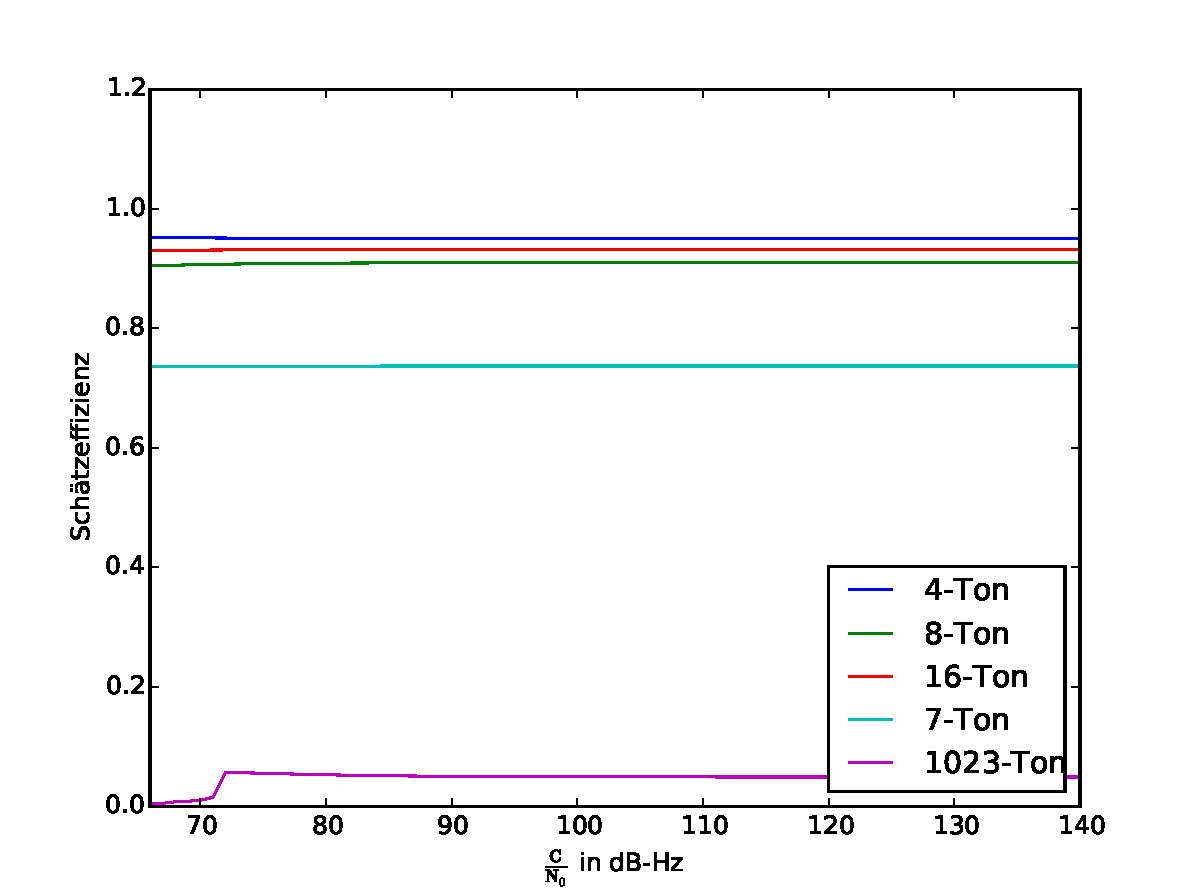
\includegraphics[width = 0.7\textwidth]{images/Schaetzeffizienz}
	\caption{Schätzeffizienz des gemittelten Phasendifferenz-Schätzers}
	\label{fig:Schätzeffizienz}
\end{figure} 

Durch Abbildung \ref{fig:Schätzeffizienz} wird ersichtlich, dass die höchste Schätzeffizienz mit dem 4-Ton erreicht wird. Zumal jedoch das Schätzverfahren beim 16-Ton eine höhere Effizienz als beim 8-Ton aufweist, kann eine steigende Subträgerzahl nicht mit einer zunehmenden Schätzeffizienz verknüpft werden. Welche Effizienz das Schätzverfahren mit einem Signal erreicht hängt lediglich von den Positionen der Subträger bzw. der Energieverteilung im Band ab.  

\subsection{Auswertung des L\texorpdfstring{$\&$}{TEXT}R-Schätzers}
\label{chap5.1.2:LundR Auswertung}
In Abbildung \ref{fig:LundR_varianz} ist der \gls{rmse} des L$\&$R-Schätzers unter Verwendung der fünf Testsignale aufgetragen. 

\begin{figure}[htbp]
	\centering
	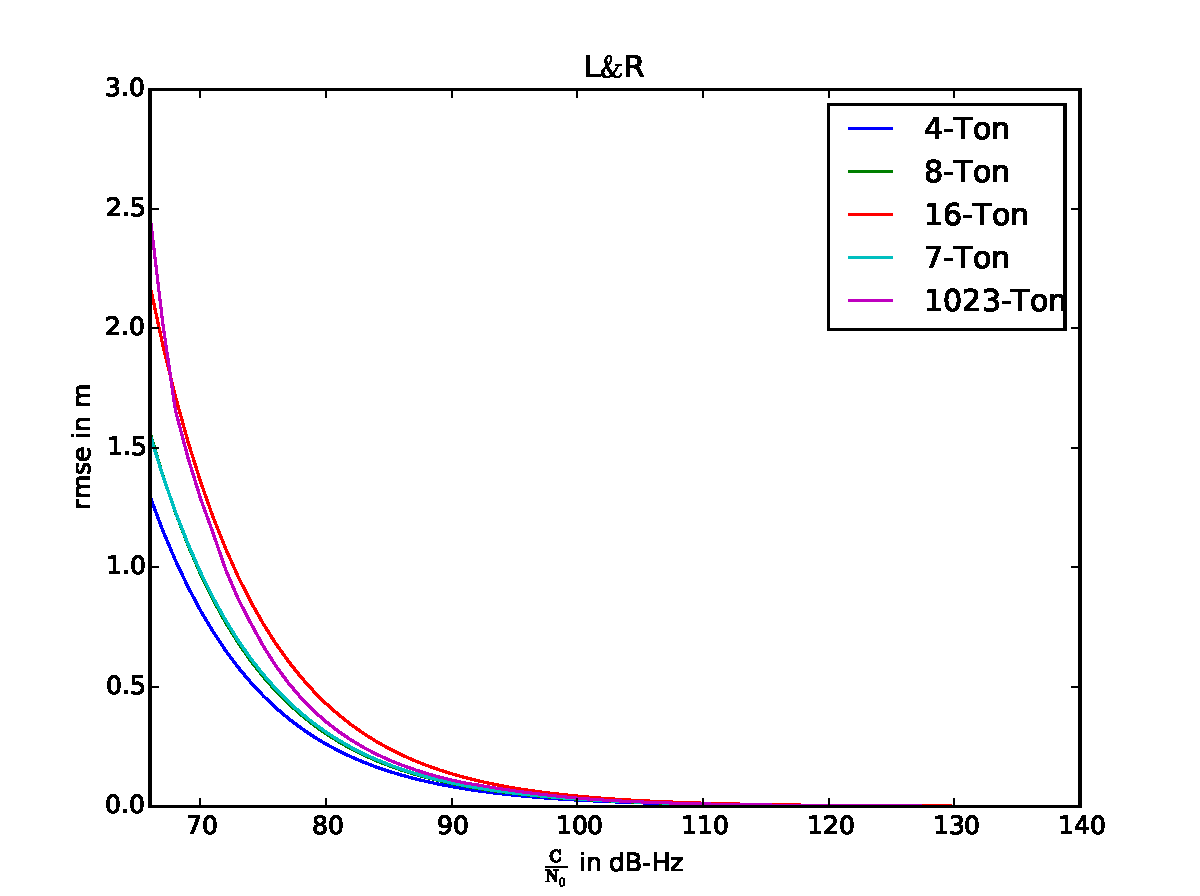
\includegraphics[width = 0.7\textwidth]{images/LundR_varianz}
	\caption{Simulation des Schätzfehlers des L$\&$R-Schätzers bei einem \gls{AWGN}-Kanal}
	\label{fig:LundR_varianz}
\end{figure}

Darin ist zu sehen, dass die $m$-Sequenzen weniger große Fehler, als beim gemittelten-Phasendifferenz-Schätzer verursachen. Um eine genauere Aussage über die Leistungsfähigkeit des L$\&$R-Schätzers zu treffen soll zunächst der Vergleich mit der \gls{CRLB} in den Abbildungen \ref{fig:Had_LuR_CRLB_vergleich} und \ref{fig:m_LuR_CRLB_vergleich} betrachtet werden. 
Die Hadamard-Sequenzen sorgen bei diesem Schätzverfahren, mit steigender Subträgerzahl, für einen größer werdenden Fehler. Die Fehlerkurven der $m$-Sequenzen kommen jedoch an die \gls{CRLB} heran.

\begin{figure}[htbp]
	\centering
	\makebox[\textwidth][c]{\begin{tabular}{cccc}
		\subfloat[4-Ton]{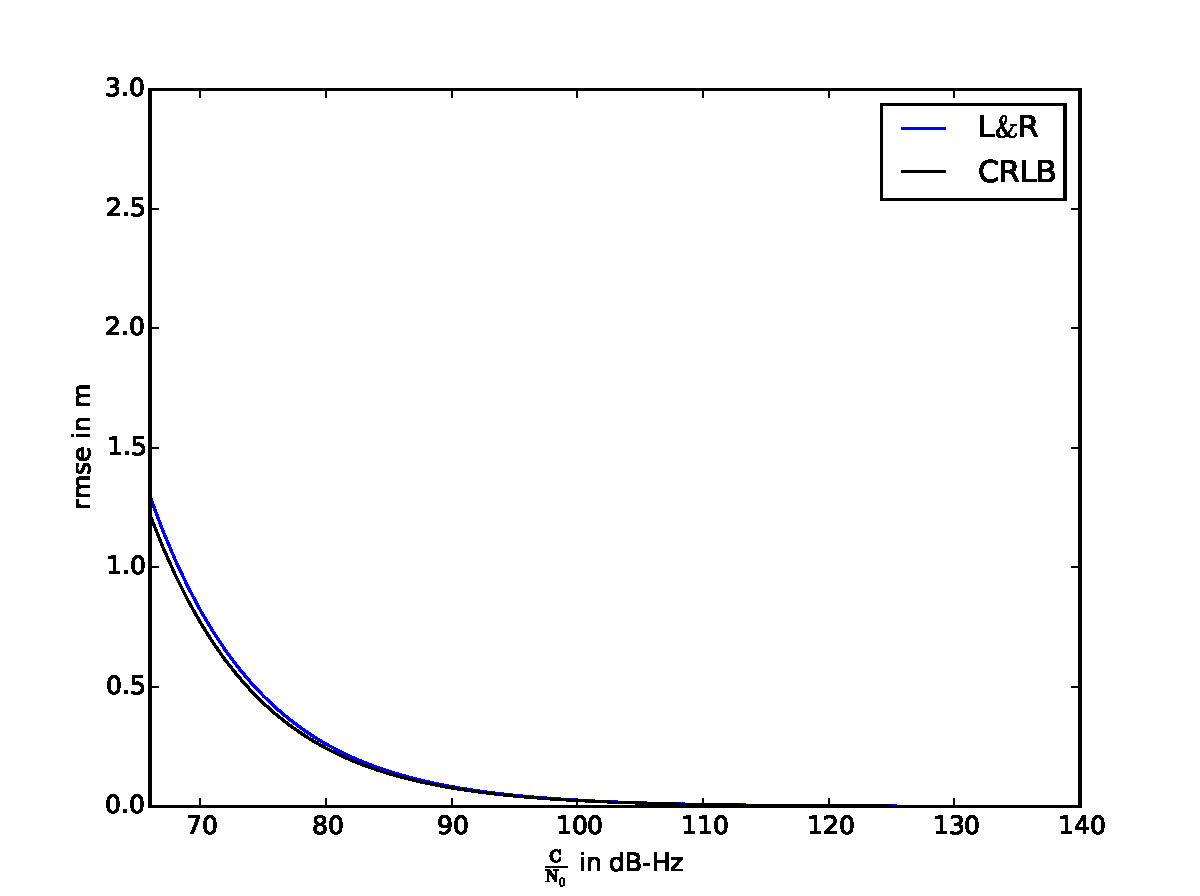
\includegraphics[width=0.5\textwidth]{images/LR4-Ton_gegen_CRLB}} &
		\subfloat[8-Ton]{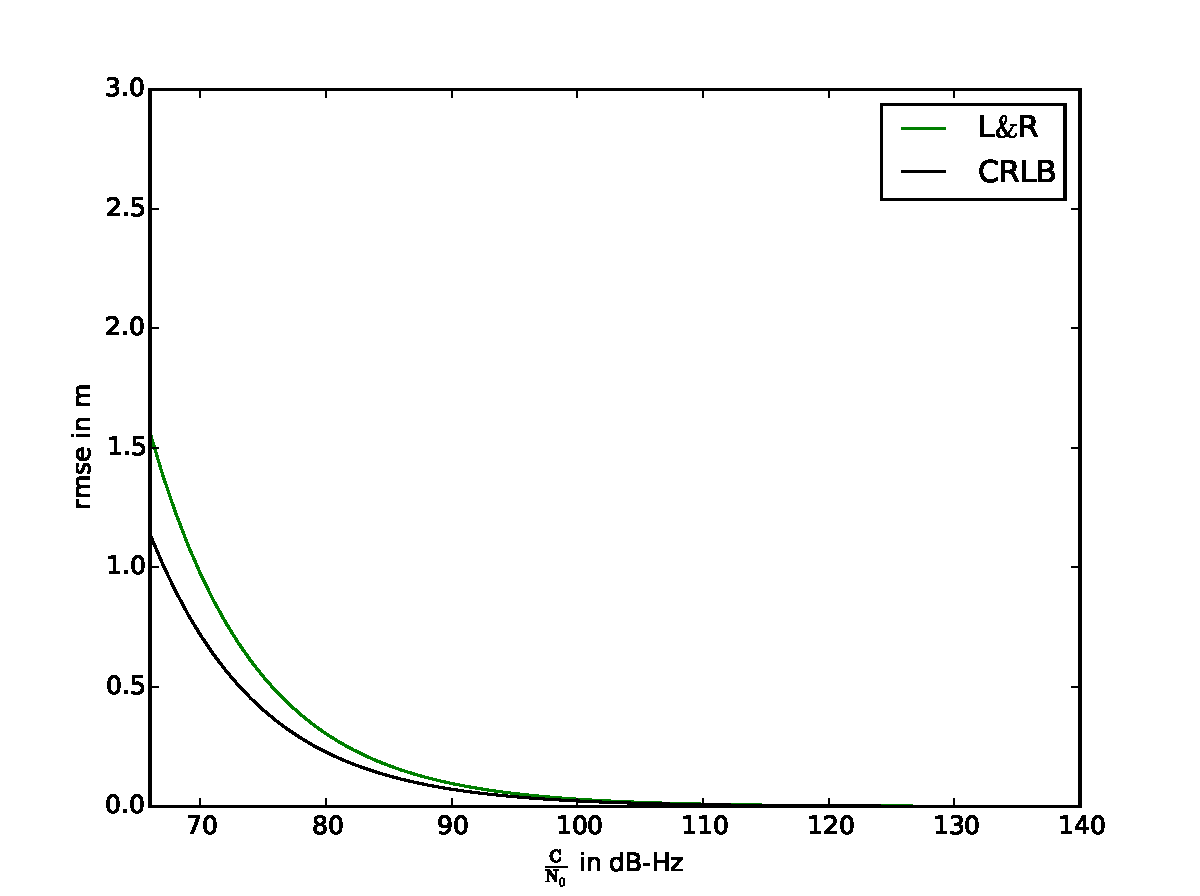
\includegraphics[width=0.5\textwidth]{images/LR8-Ton_gegen_CRLB}}
	\end{tabular}}
		
	\makebox[\textwidth][c]{\begin{tabular}{cccc}
		\subfloat[16-Ton]{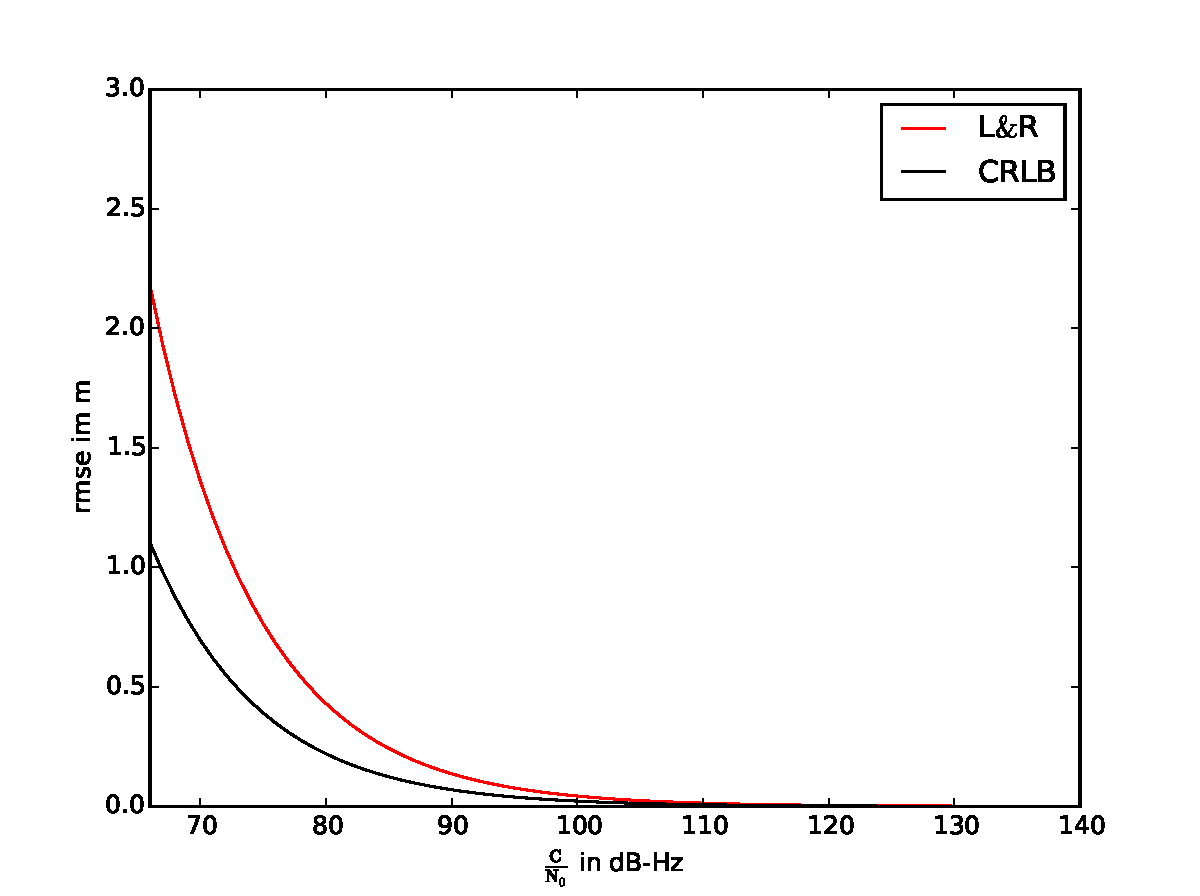
\includegraphics[width=0.5\textwidth]{images/LR16-Ton_gegen_CRLB}}
	\end{tabular}}
	
	\caption{\gls{rmse} des L$\&$R-Schätzers mit Hadamard-Sequenzen gegenüber der \gls{CRLB}}
	\label{fig:Had_LuR_CRLB_vergleich}	
\end{figure}

Eine Erklärungsmöglichkeit für die schlechten Ergebnisse der Hadamard-Sequenzen, kann in der Gleichung \eqref{eq:Approximation} gefunden werden. Darin wird eine Vereinfachung für eine Summe von Exponentialfunktionen vorgenommen. Der Ansatz geht jedoch davon aus, dass alle $e$-Funktionen gleich gewichtet sind. Da die Subträger der Hadamard-Sequenzen unterschiedliche Gewichte haben, trifft diese Vereinfachung nicht auf diese Signalform zu. Bei zunehmender Subträgerzahl werden diese Abweichungen immer größer. Um das Schätzverfahren trotzdem auswerten zu können, wurden die Subträger der Signale nachträglich skaliert, damit sie die selben Gewichte haben. Diese Maßnahme verschlechtert jedoch das \nicefrac[]{\gls{symb:C}}{\gls{symb:N0}}, da das Rauschen ebenfalls skaliert wird. Diese Fehlerquelle zeigt, dass der \gls{LuR}-Schätzer suboptimal für diese Art von Signalen ist. Um den \gls{rmse} an die \gls{CRLB} anzunähern, müsste die Approximation \eqref{eq:Approximation} nochmals für unterschiedlich gewichtete e-Funktionen hergeleitet werden. Dies überschreitet jedoch den Umfang dieser Arbeit, da nicht einmal erwiesen ist, ob eine solche Vereinfachung für unterschiedlich gewichtete Exponentialfunktionen überhaupt existiert. 

\begin{figure}[htbp]
	\centering
	\makebox[\textwidth][c]{\begin{tabular}{ccc}
		\subfloat[7-Ton]{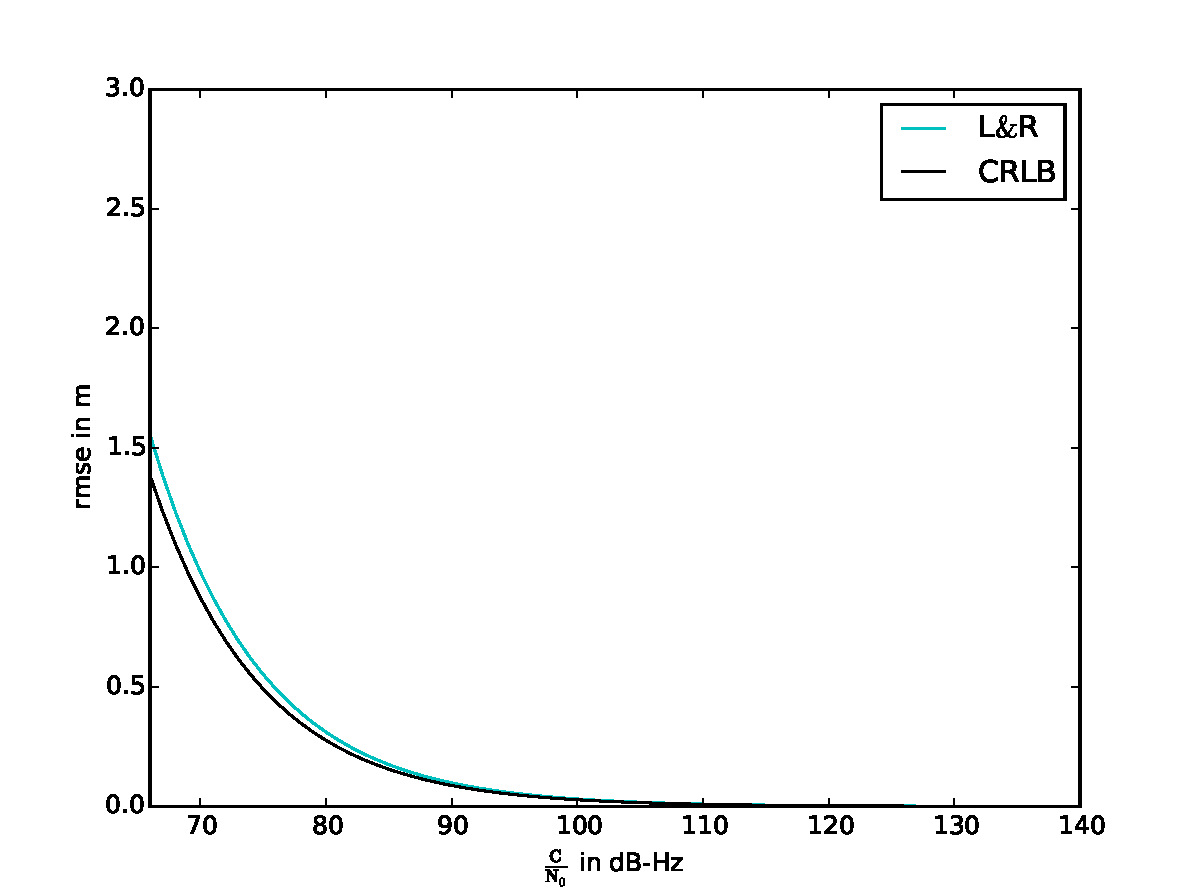
\includegraphics[width=0.5\textwidth]{images/LR7-Ton_gegen_CRLB}} &
		\subfloat[1024-Ton]{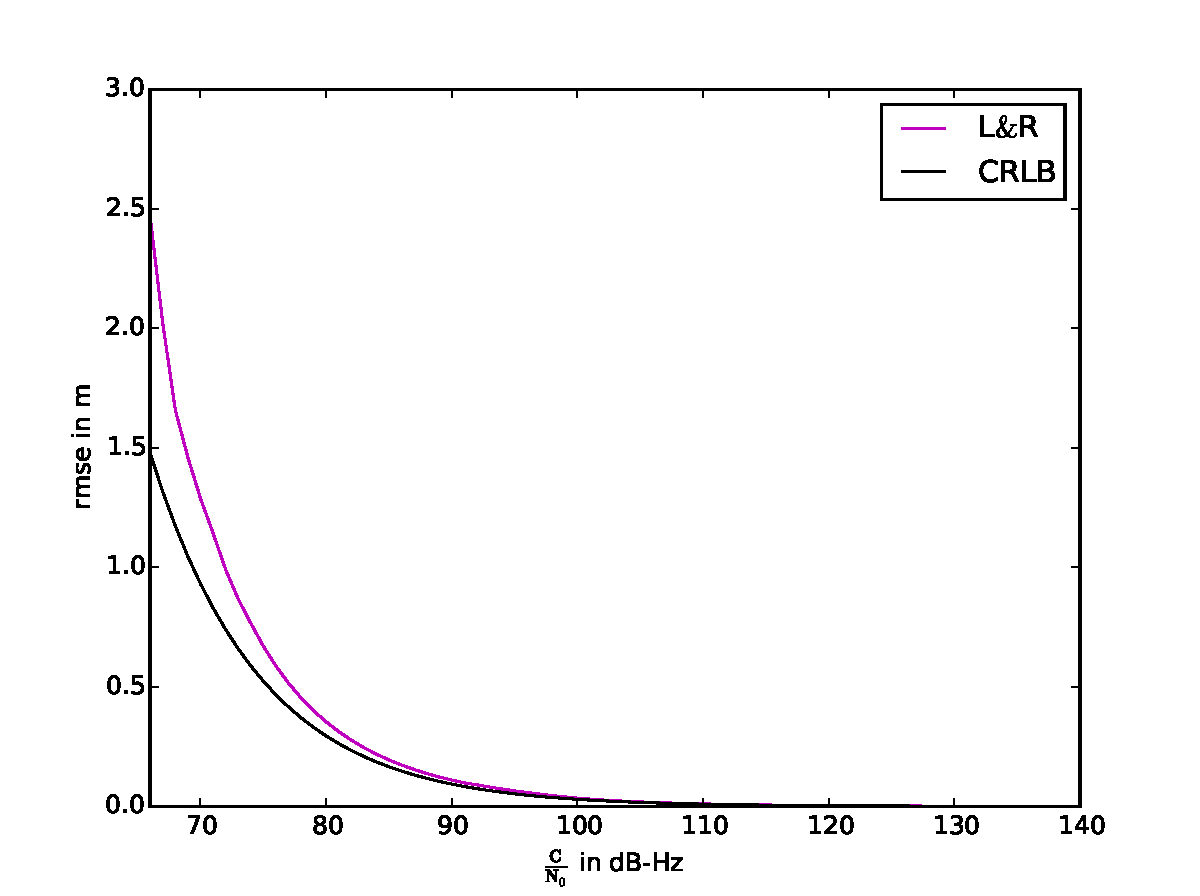
\includegraphics[width=0.5\textwidth]{images/LR1023-Ton_gegen_CRLB}}
	\end{tabular}}
	\caption{\gls{rmse} des L$\&$R-Schätzers mit $m$-Sequenzen gegenüber der \gls{CRLB}}
	\label{fig:m_LuR_CRLB_vergleich}
\end{figure}

Die $m$-Sequenzen erfüllen die Bedingung zwar bei ihrer Erzeugung, sind jedoch nach der Impulsformung mit einer Sinc-Funktion im Frequenzbereich gewichtet. Daher gilt diese Vereinfachung für sie ebenfalls nicht. Der Fehler scheint allerdings bei ihnen nicht so stark ins Gewicht zu fallen. Laut \cite[S.90]{mengali1997synchronization} ist die wesentliche Verbesserung dieses Schätzverfahrens gegenüber anderen Mittelungsverfahren, dass das \nicefrac[]{\gls{symb:C}}{\gls{symb:N0}}, durch die zusätzliche Glättung des Rauschens in Gleichung \eqref{eq:rauschglaettung} verbessert wird. Dies könnte eine Begründung dafür sein, wieso sich die $m$-Sequenzen im Vergleich zum gemittelten-Phasendifferenz-Schätzers, so stark verbessern, obwohl sie ungleiche Subträgergewichte aufweisen. Zum einen ist der Unterschied der Subträgergewichte nach der Impulsformung nicht so groß wie bei den Hadamard-Sequenzen und zum anderen besitzen sie mehr Phasenwerte, über welche gemittelt werden kann. 
An der Schätzeffizienz in Abbildung \ref{fig:LuRSChätzeffizienz} ist zu sehen wie stark die $m$-Sequenzen sich verbessern. Bei dem 7-Ton ist die Verbesserung nur noch minimal, da diese Signalform beim gemittelten Phasendifferenz-Schätzer schon einen Verlauf ähnlich der \gls{CRLB} hatte.
Aus der Schätzeffizienz aller Signale kann wiederum bestimmt werden, welche die geeignetste Signalform für diesen Schätzer ist. 
\begin{figure}[htbp]
	\centering
	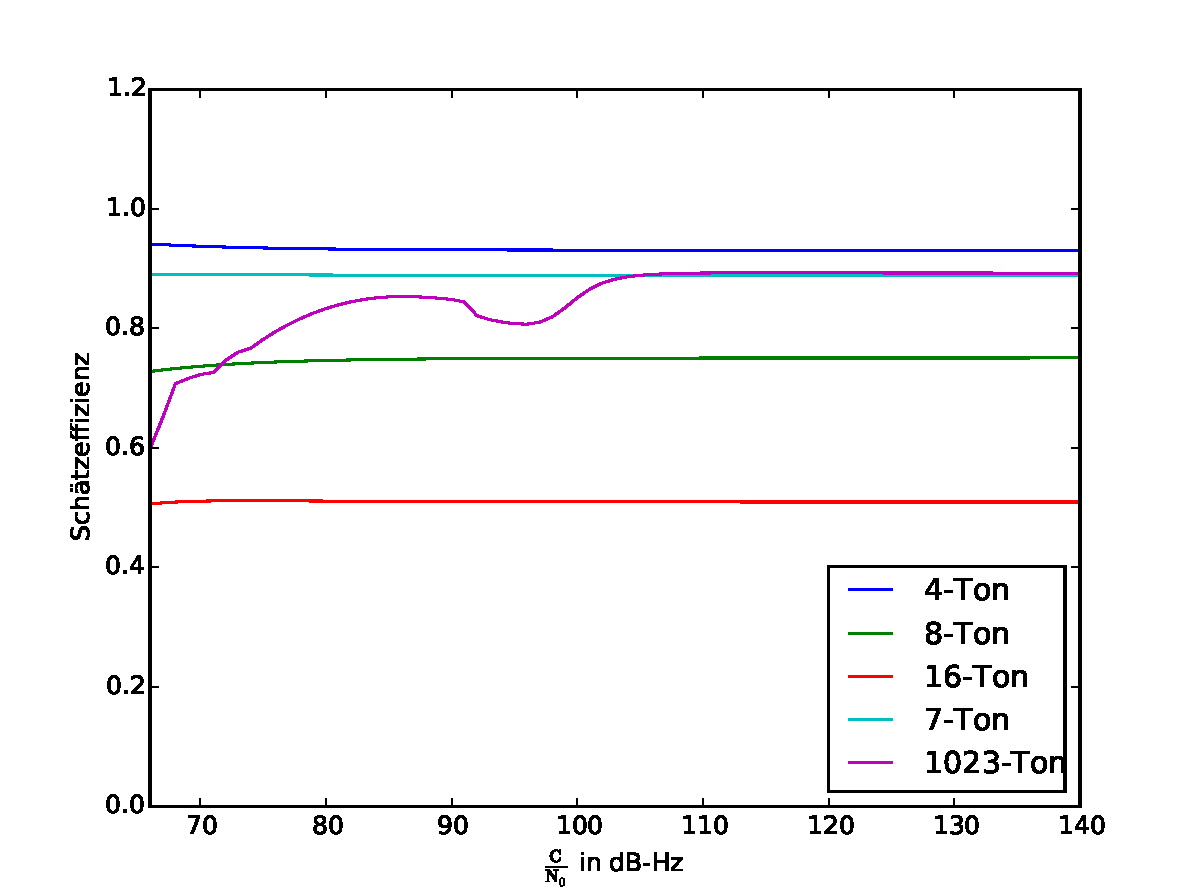
\includegraphics[width = 0.7\textwidth]{images/LuRschaetzeffizienz}
	\caption{Schätzeffizienz des L$\&$R-Schätzers}
	\label{fig:LuRSChätzeffizienz} 
\end{figure}
Die Effizienz des 1023-Ton ist für ein gutes \nicefrac[]{\gls{symb:C}}{\gls{symb:N0}} sehr hoch, fällt jedoch bei kleiner werdenden \nicefrac[]{\gls{symb:C}}{\gls{symb:N0}} stark ab. Der 7-Ton und 4-Ton weisen die höchste Effizienz bei diesen Schätzverfahren auf. Im Vergleich zu ihnen, sind die Signale des 8- und 16-Tons äußerst ineffizient.

\subsection{Auswertung von MUSIC und ESPRIT}
\gls{MUSIC} und \gls{ESPRIT} arbeiten im selben Subraum und haben deshalb ähnliche Ergebnisse in der Auswertung. Lediglich die Art und Weise, wie die Laufzeitinformation aus dem Subraum extrahiert wird, unterscheidet sich bei diesen Verfahren.

\begin{figure}[htbp]
	\centering
	\makebox[\textwidth][c]{\begin{tabular}{ccc}
		\subfloat[\gls{MUSIC}]{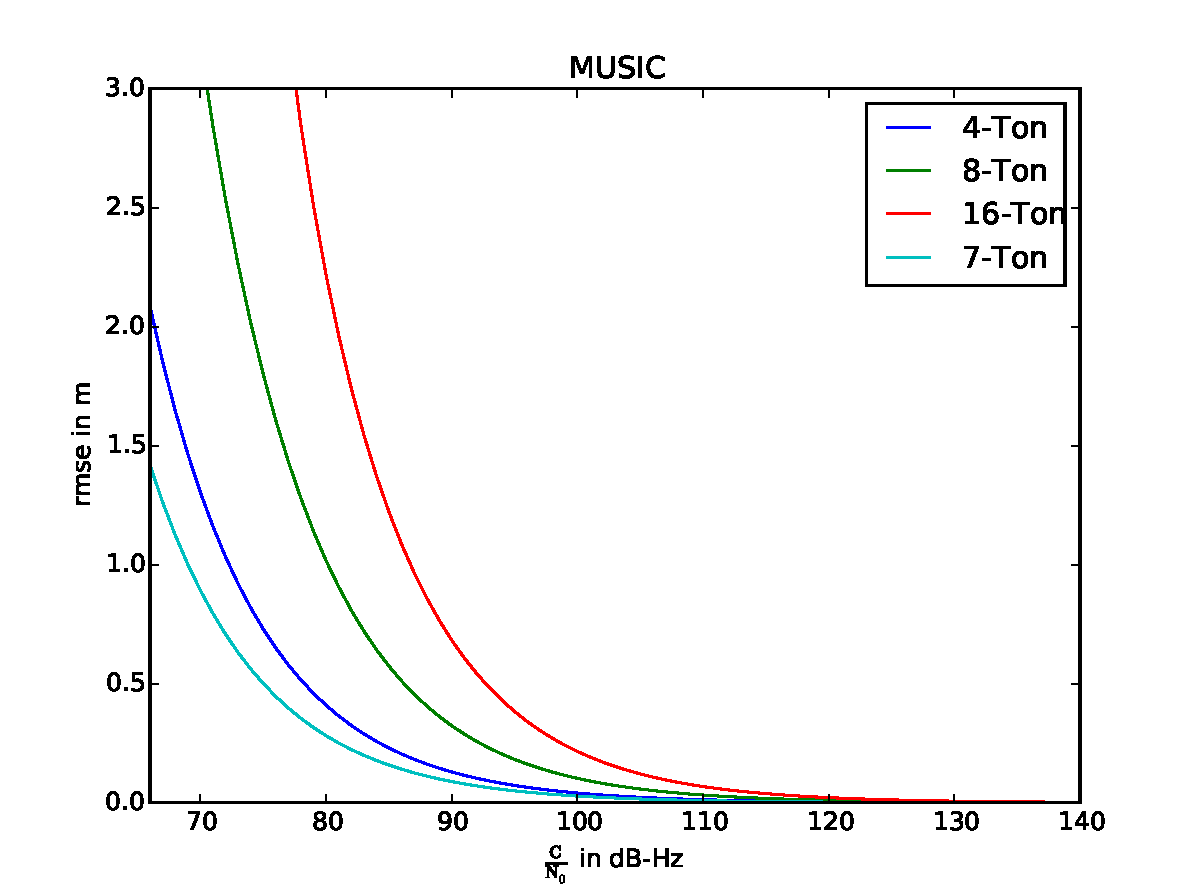
\includegraphics[width = 0.5\textwidth]{images/MUSIC_varianz}} &
		\subfloat[\gls{ESPRIT}]{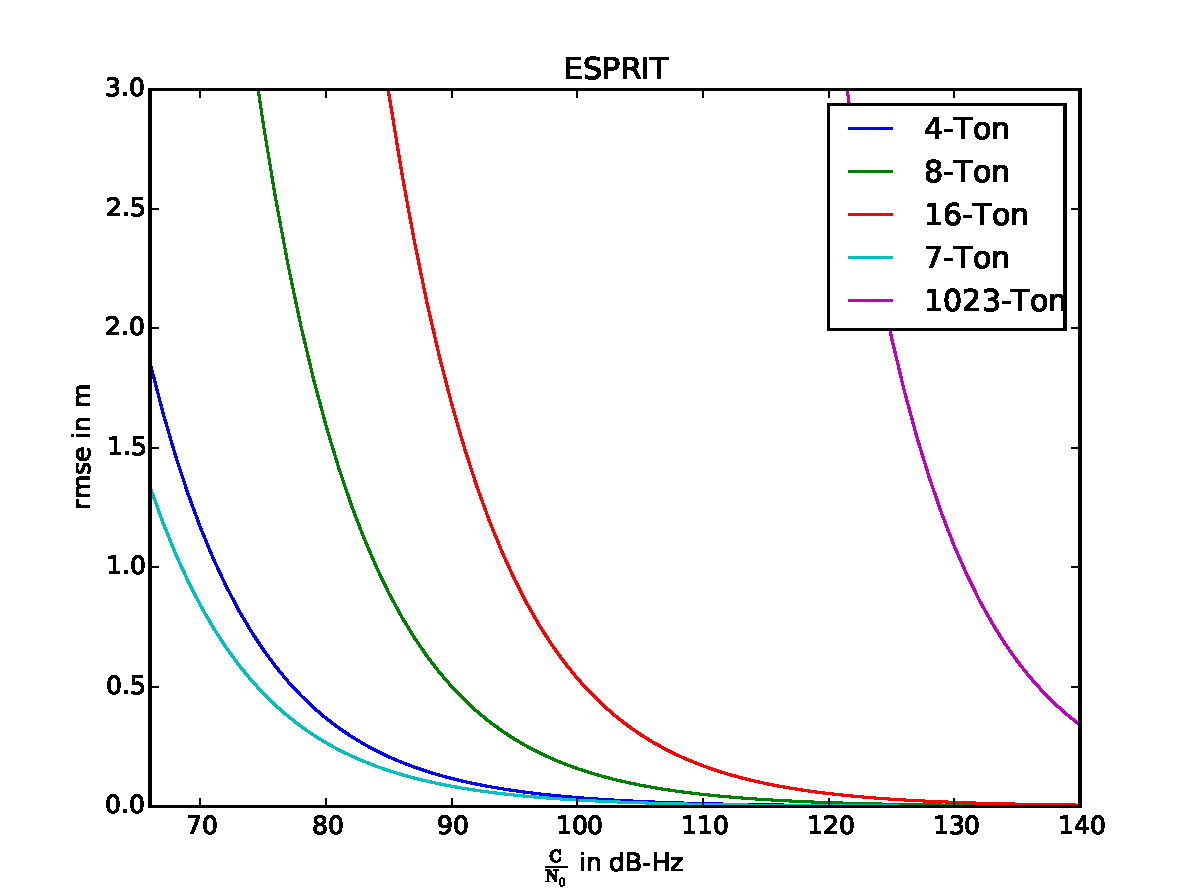
\includegraphics[width = 0.5\textwidth]{images/ESPRIT_varianz}}
	\end{tabular}}
	\caption{Simulation des Schätzfehlers des \gls{ESPRIT}- und \gls{MUSIC}-Schätzers bei einem \gls{AWGN}-Kanal}
	\label{fig:ESPRIT_MUSIC_varianz}
\end{figure}

In Abbildung \ref{fig:ESPRIT_MUSIC_varianz} ist zu sehen, dass die Kurven ähnliche Verläufe aufzeigen. Eine Auswertung für den 1023-Ton  war mit dem Root-\gls{MUSIC} Algorithmus jedoch nicht möglich, da dieser mit der hohen Anzahl an Subträgern einen zu hohen Rechenaufwand benötigt. 
Die Fehlerkurven aller Signale steigen bei kleinen \nicefrac[]{\gls{symb:C}}{\gls{symb:N0}} stark an. Zunächst wird \gls{ESPRIT} ausgewertet.
Lediglich der 7-Ton bleibt in der Nähe der \gls{CRLB}, wie in den Abbildungen \ref{fig:Had_ESPRIT_CRLB_vergleich} und \ref{fig:m_ESPRIT_CRLB_vergleich} zu sehen ist. 

\begin{figure}[htbp]
	\centering
	\makebox[\textwidth][c]{
	\begin{tabular}{cccc}	
		\subfloat[4-Ton]{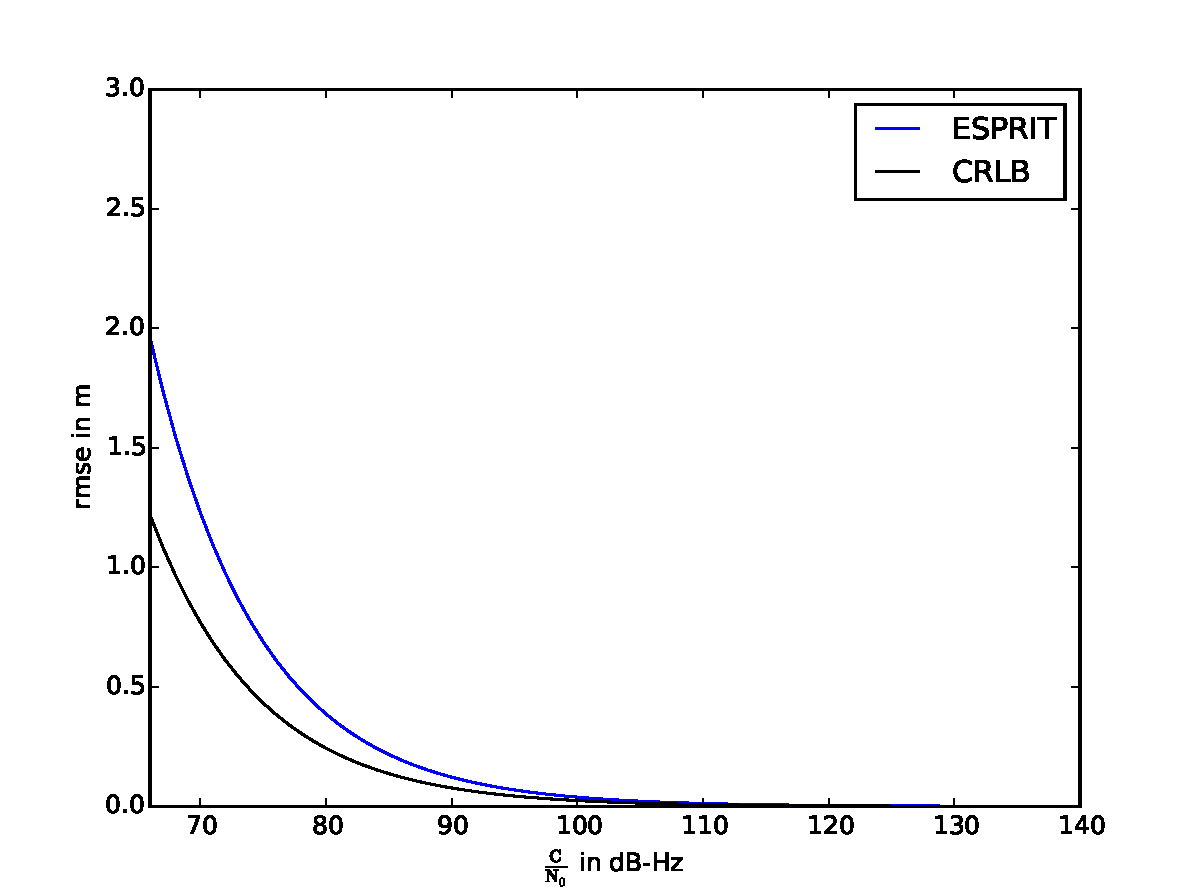
\includegraphics[width = 0.5\textwidth]{images/ESPRIT_4Ton_CRLB}} &
		\subfloat[8-Ton]{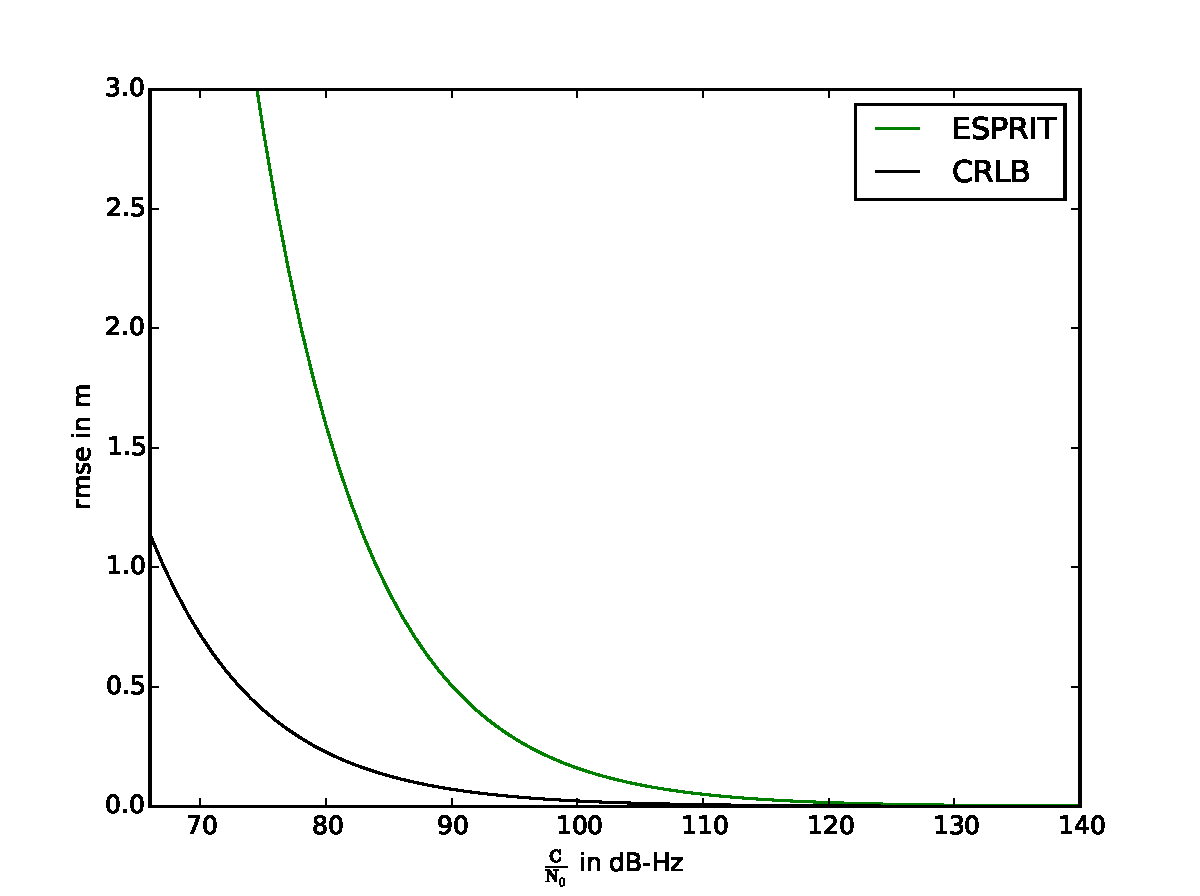
\includegraphics[width = 0.5\textwidth]{images/ESPRIT_8Ton_CRLB}}
		\end{tabular}}	
		
	\makebox[\textwidth][c]{\begin{tabular}{ccc}
		\subfloat[16-Ton]{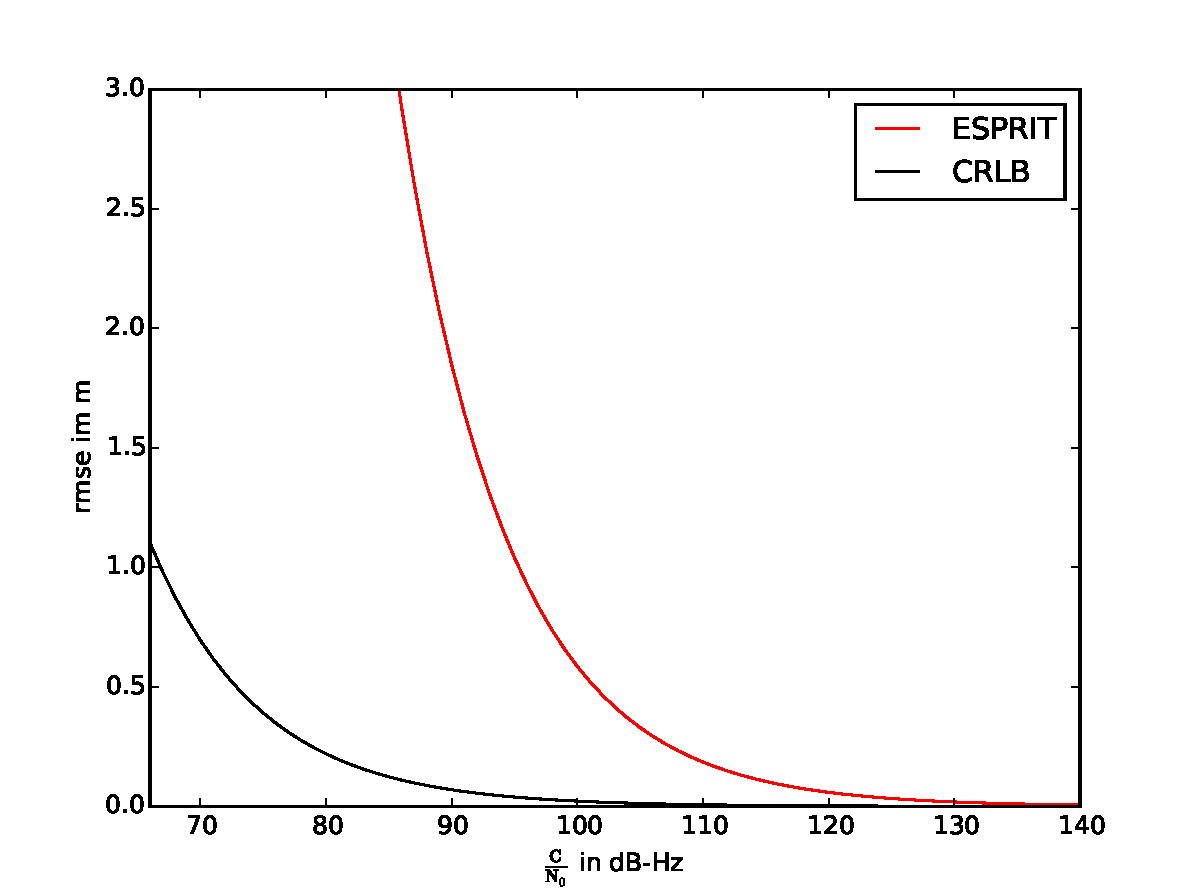
\includegraphics[width = 0.5\textwidth]{images/ESPRIT_16Ton_CRLB}}
			\end{tabular}}
	\caption{Varianz des \gls{ESPRIT}-Schätzers gegenüber der \gls{CRLB} für Hadamard-Sequnzen}
	\label{fig:Had_ESPRIT_CRLB_vergleich}
\end{figure}

Auffällig ist, dass die Hadamard-Sequenzen besonders stark von der \gls{CRLB} abweichen.
Bei genauerer Betrachtung des Schätzablaufes, wird ersichtlich, dass ein Fehler bei der Kanalschätzung, nach \eqref{eq:Übertragungsfunktion}, gemacht wird, wenn die Subträger nicht gleich gewichtet sind. Es handelt sich wieder um ein ähnliches Problem, wie beim \gls{LuR}-Schätzer. Wenn die Subträger nicht gleich gewichtet sind, wird bei der Bildung des Quotienten, jeder Subträger mit sich selbst normiert. Dadurch werden Subträger skaliert und verschlechtern somit das \nicefrac[]{\gls{symb:C}}{\gls{symb:N0}}. Als Lösung dieses Problems, würde sich anbieten anstelle der Quotientenbildung ein komplex konjugiertes Produkt des Empfangsspektrums $R(f)$ und des Sendespektrums $S(f)$ zu berechnen. Damit gehen jedoch erhebliche Veränderungen an den Algorithmen einher.  Anstrengungen dieses Problem zu umgehen, führten allerdings zu keiner Verbesserung des Schätzfehlers. Somit zeigt der \gls{rmse} dieses Schätzers, dass die Algorithmen Signale mit gleich gewichteten Subträgern benötigen. 

\begin{figure}[htbp]
	\centering
	\makebox[\textwidth][c]{	
	\begin{tabular}{cccc}
		\subfloat[7-Ton]{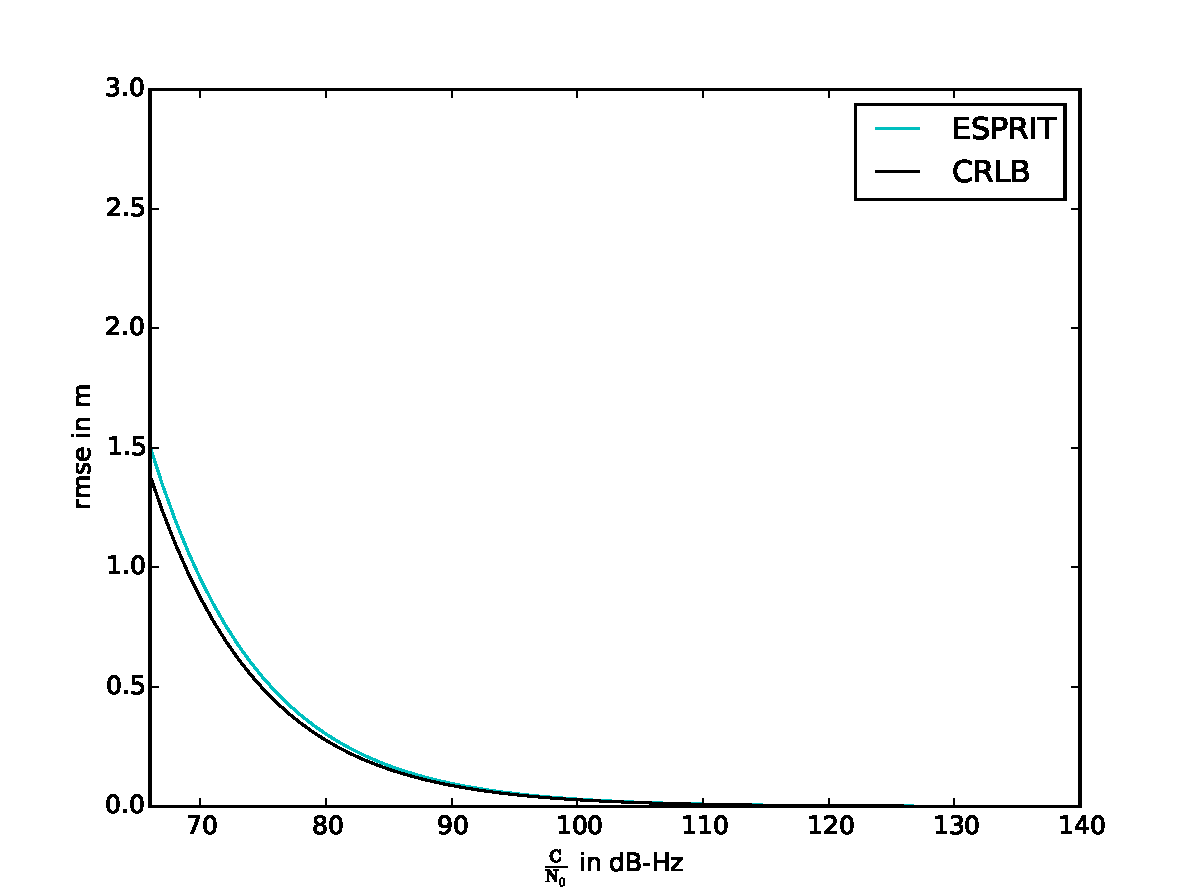
\includegraphics[width = 0.5\textwidth]{images/ESPRIT_7Ton_CRLB}} &
		\subfloat[1025-Ton]{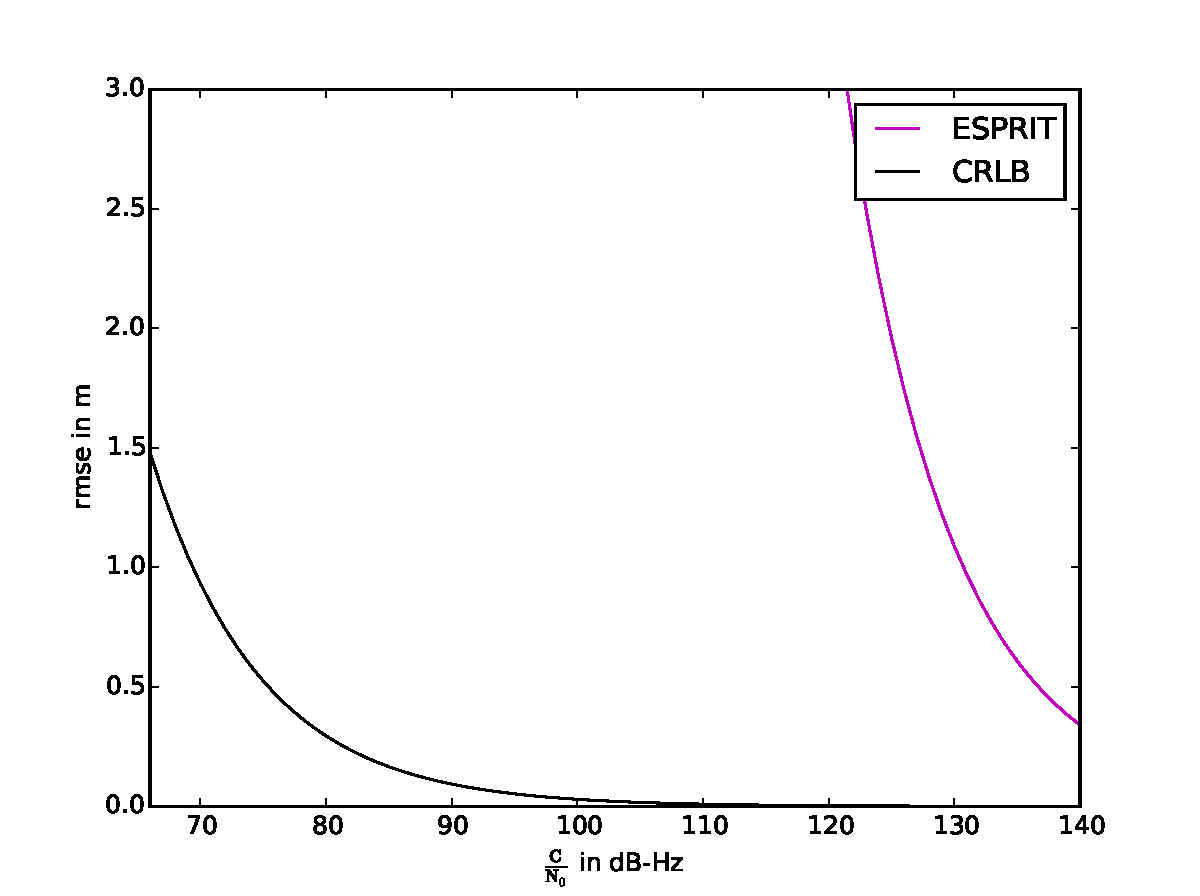
\includegraphics[width = 0.5\textwidth]{images/ESPRIT_1023Ton_CRLB}}	
	\end{tabular}}
	\caption{Varianz des \gls{ESPRIT}-Schätzers gegenüber der CRLB für $m$-Sequnzen}
	\label{fig:m_ESPRIT_CRLB_vergleich}
\end{figure}

Wie bereits festgestellt haben die Fehlerkurven des \gls{MUSIC}-Algorithmus einen ähnlichen Verlauf, wie die bei \gls{ESPRIT}. An der Abbildung \ref{fig:MUSIC_CRLB_vergleich} ist jedoch zu erkennen, dass sie etwas näher an der \gls{CRLB} liegen.  

\begin{figure}[htbp]
	\centering
	\makebox[\textwidth][c]{
	\begin{tabular}{cccc}	
		\subfloat[4-Ton]{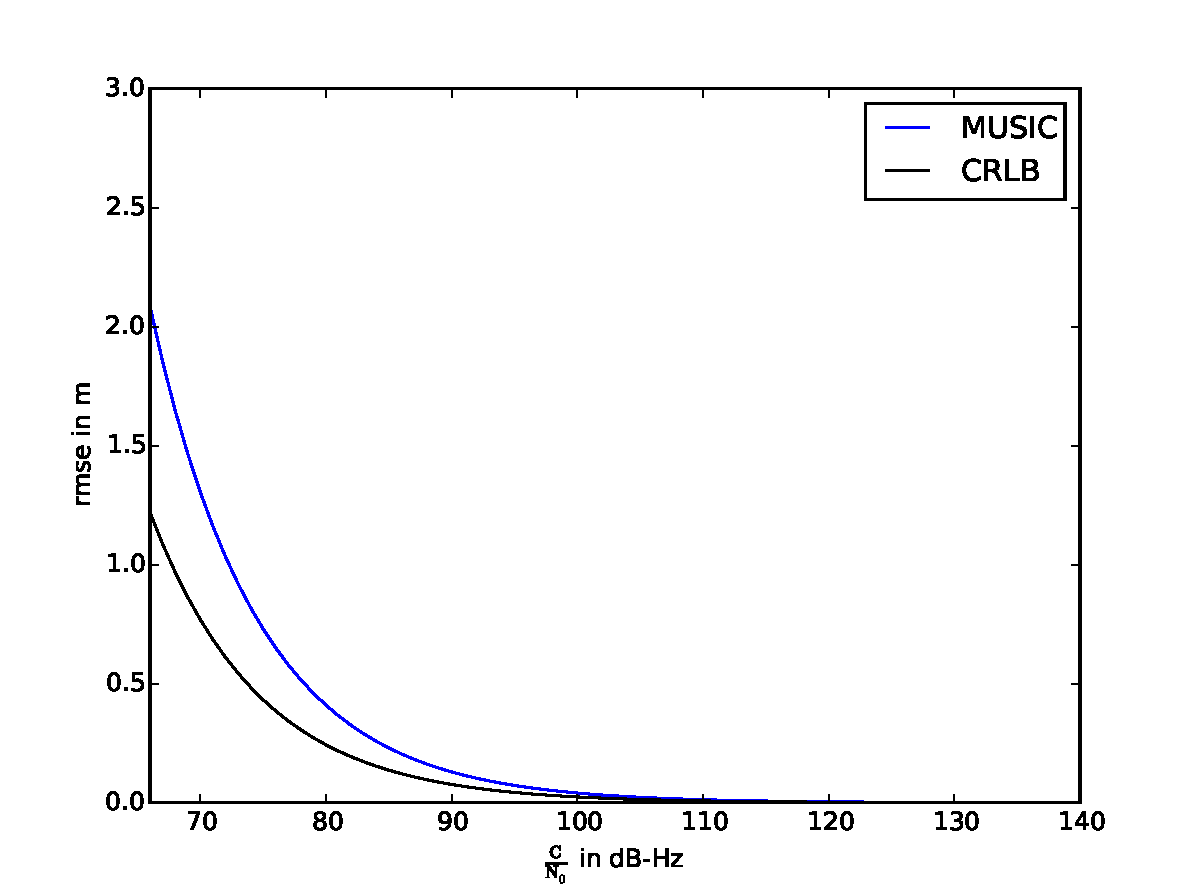
\includegraphics[width = 0.5\textwidth]{images/MUSIC_4Ton_CRLB}} &
		\subfloat[8-Ton]{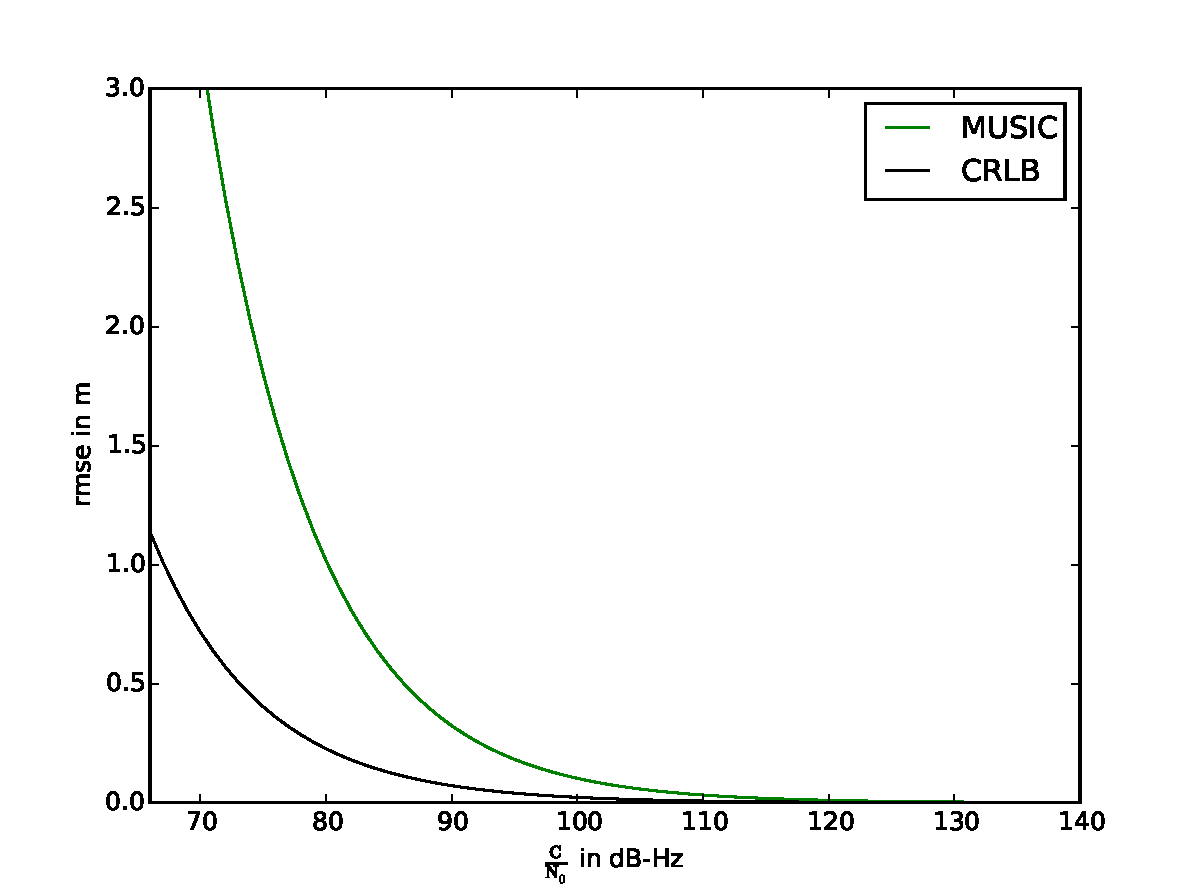
\includegraphics[width = 0.5\textwidth]{images/MUSIC_8Ton_CRLB}} \\		
		\subfloat[16-Ton]{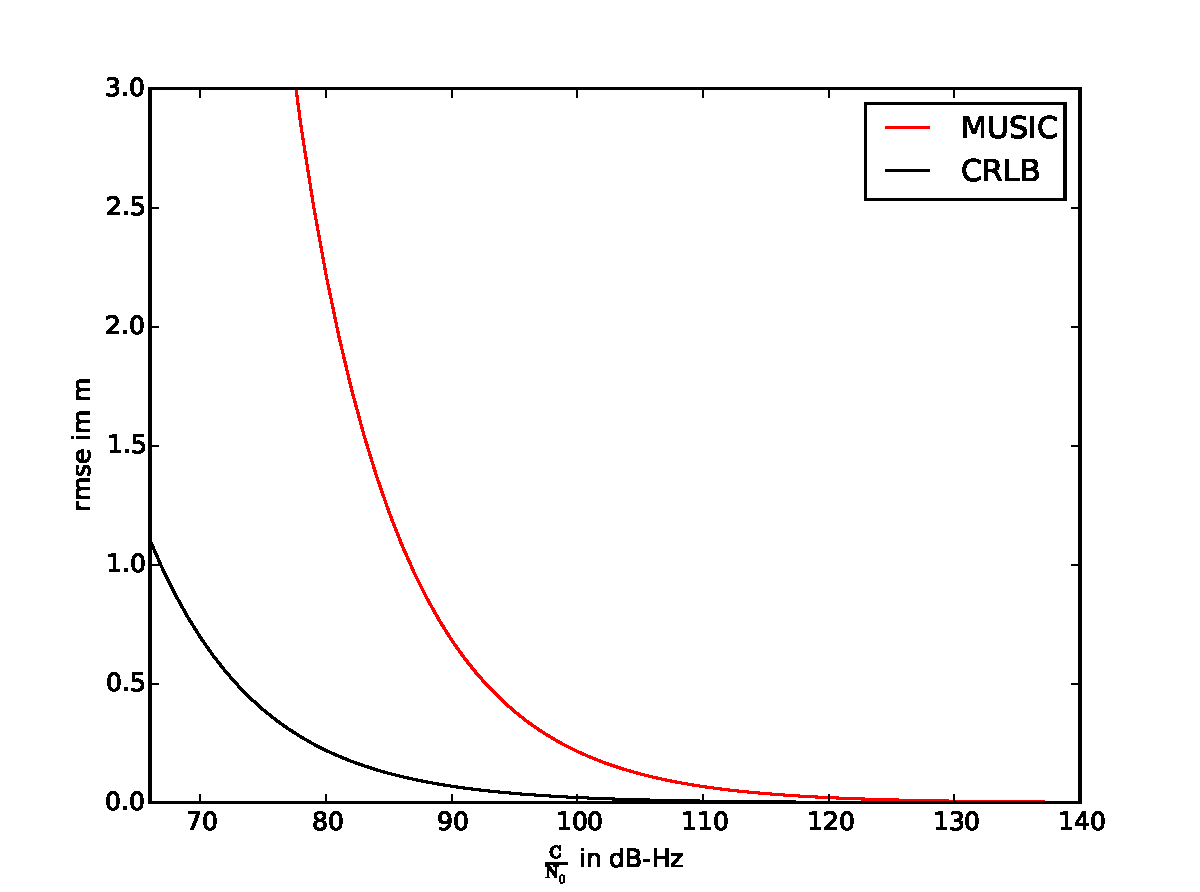
\includegraphics[width = 0.5\textwidth]{images/MUSIC_16Ton_CRLB}} &
		\subfloat[7-Ton]{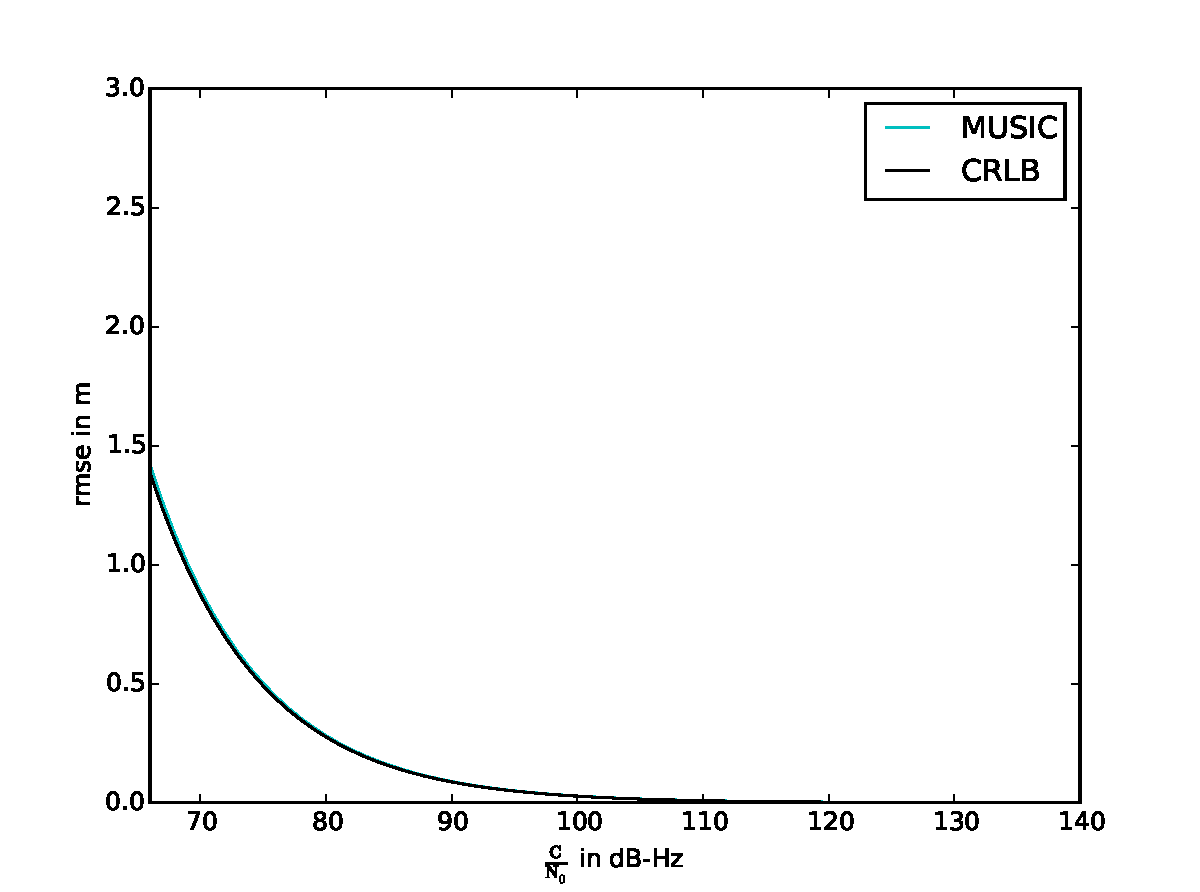
\includegraphics[width = 0.5\textwidth]{images/MUSIC_7Ton_CRLB}}
		\end{tabular}}		
	\caption{Varianz des \gls{MUSIC}-Schätzers gegenüber der \gls{CRLB}}
	\label{fig:MUSIC_CRLB_vergleich}
\end{figure}

Aufgrund der vorangegangenen Auswertungen der Subraummethoden kann geschlussfolgert werden, dass der 7-Ton die einzige Signalform ist, welche mit diesen Verfahren gute Ergebnisse erzielt. Dies lässt sich auch aus der Schätzeffizienz dieser Schätzverfahren für die unterschiedlichen Signale, wie in Abbildung \ref{fig:Schätzeffizienz_Subraum} ablesen. Bei beiden Algorithmen hat der 7-Ton die höchste Effizienz. \gls{MUSIC} übertrifft jedoch \gls{ESPRIT} minimal.

\begin{figure}[htbp]
	\centering
	\makebox[\textwidth][c]{\begin{tabular}{ccc}
		\subfloat[\gls{ESPRIT}]{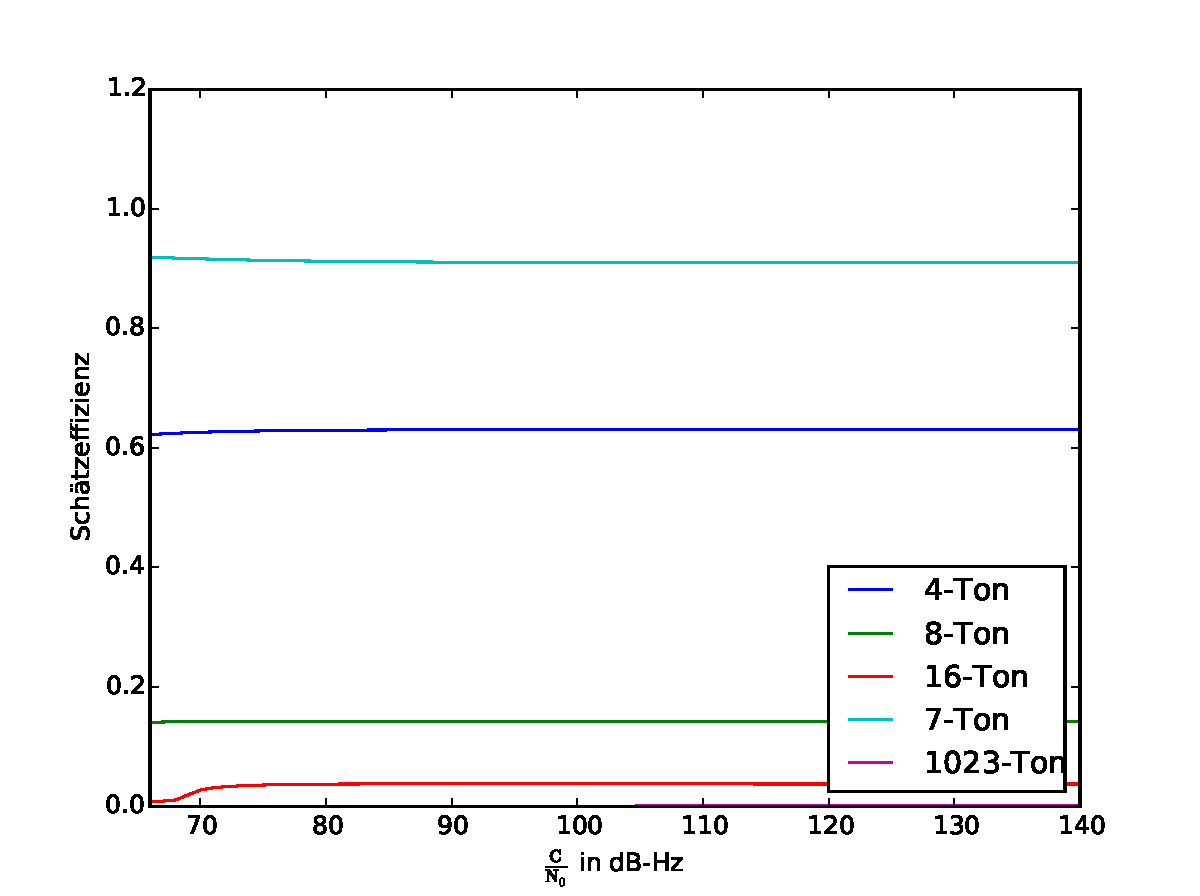
\includegraphics[width = 0.5\textwidth]{images/Schaetzeffizienz_ESPRIT}} &
		\subfloat[\gls{MUSIC}]{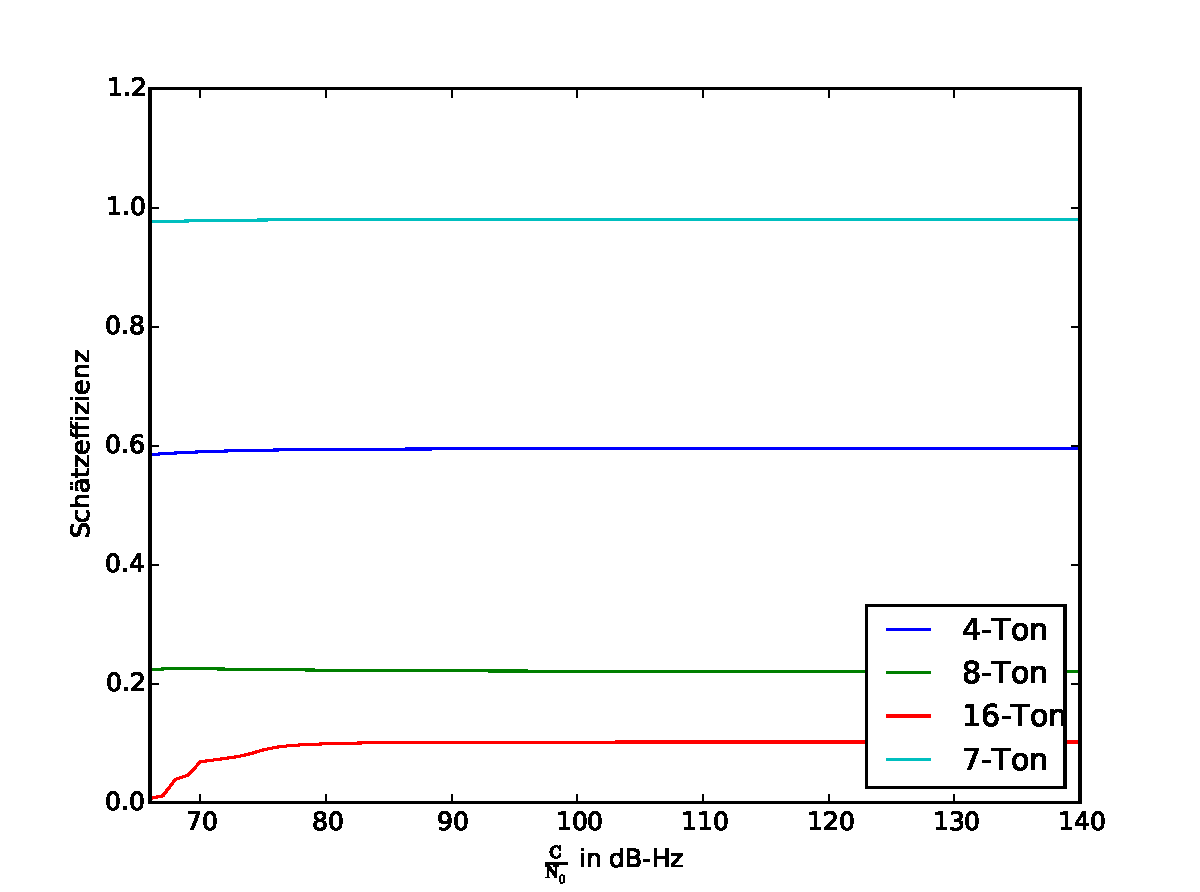
\includegraphics[width = 0.5\textwidth]{images/Schaetzeffizienz_MUSIC}}
	\end{tabular}}
	
	\caption{Schätzeffizienz der Subraumalgorithmen}
	\label{fig:Schätzeffizienz_Subraum}	
\end{figure}



\subsection{Auswertung für den \gls{AWGN}-Fall}

Der gemittelte-Phasendifferenz-Schätzer ist stark von der Energieverteilung auf die jeweiligen Subträger abhängig und macht bei einem fast weißen Spektren einen sehr großen Fehler. Der \gls{LuR}-Schätzer schafft es allerdings gerade bei diesen Sequenzen das \nicefrac[]{\gls{symb:C}}{\gls{symb:N0}} erheblich zu verbessern und ist daher im \gls{AWGN}-Fall deutlich weniger fehleranfällig. Ein großer Nachteil des \gls{LuR}-Schätzers, ist jedoch eine Vereinfachung, die getroffen wird, welche bei Hadamard-Sequenzen nicht angewendet werden kann. Gerade diese Sequenzen haben aber besonders gute Eigenschaften um Fehler im \gls{AWGN}-Kanal zu minimieren.
Zusätzlich stellt sich die Impulsformung mit einem Rechteck auch als suboptimal für diesen Schätzer heraus. Um die Stärken des \gls{LuR}-Schätzers voll auszuschöpfen, müssen Signale erzeugt werden, die auch nach der Impulsformung gleich gewichtete Subträger besitzen.    
Auch die Subraummethoden haben Schwierigkeiten mit den Hadamard-Sequenzen, da ein ähnlicher Fehler wie beim \gls{LuR}-Schätzer gemacht wird. Anders als beim \gls{LuR}-Schätzer können die schlechten \gls{AWGN}-Eigenschaften des 1023-Tons nicht verbessert werden und führen dementsprechend zu großen Fehlern bei kleinen \nicefrac[]{\gls{symb:C}}{\gls{symb:N0}}. Am besten funktionieren die Subraummethoden mit einem 7-Ton. 

\section{Betrachtung bei Mehrwegeausbreitung}
\label{chap5.2:Mehrwege}
In Abschnitt \ref{chap2.3.3:Hüllkurven} wurde bereits diskutiert, dass die \gls{CRLB} kein sinnvolles Maß zum quantifizieren eines Schätzer unter Einfluss eines Mehrwegekanals ist. An ihrer Stelle werden Fehlerhüllkurven erzeugt, um das, von unterschiedlichen Parametern abhängige, Verhalten der Schätzer genauer zu untersuchen. Diese Hüllkurven erlauben es zwar nicht, eine Aussage darüber zu treffen, ob ein Schätzer der Bestmögliche hinsichtlich eines \gls{mvue} ist, sie geben aber Aufschluss darüber, ob die Schätzer untereinander Vor- oder Nachteile aufweisen. Zudem kann eine Aussage darüber getroffen werden, ob die Fehler, die entstehen können, in einem realen System zu tolerieren sind. Der untersuchte Mehrwegekanal besteht aus zwei Pfaden. Der Zweite Pfad hat den Betrag $\alpha = 0,5$. Diese Annahme legt das Verhältnis des \gls{SNR} vom \gls{LOS} zum \gls{SNR} des Umwegpfad fest, was jedoch realitätsfern ist. Das \gls{SNR} des Umwegpfades ist in der Realität distanzabhängig. Die Annahme vereinfacht jedoch das Modell und liefert allgemeine Erkenntnisse und Tendenzen über das Mehrwegeauflösungsvermögen der Schätzer.

\subsection{Auswertung des gemittelten-Phasendifferenz-Schätzers}
\label{chap:5.2.1:gemittelte Phasendifferenz}
Zunächst sollen die Hüllkurven im Basisband betrachtet werden, um anschließend Einflusse der Trägerfrequenz erkennen zu können. 

\begin{figure}[htbp]
	\centering
	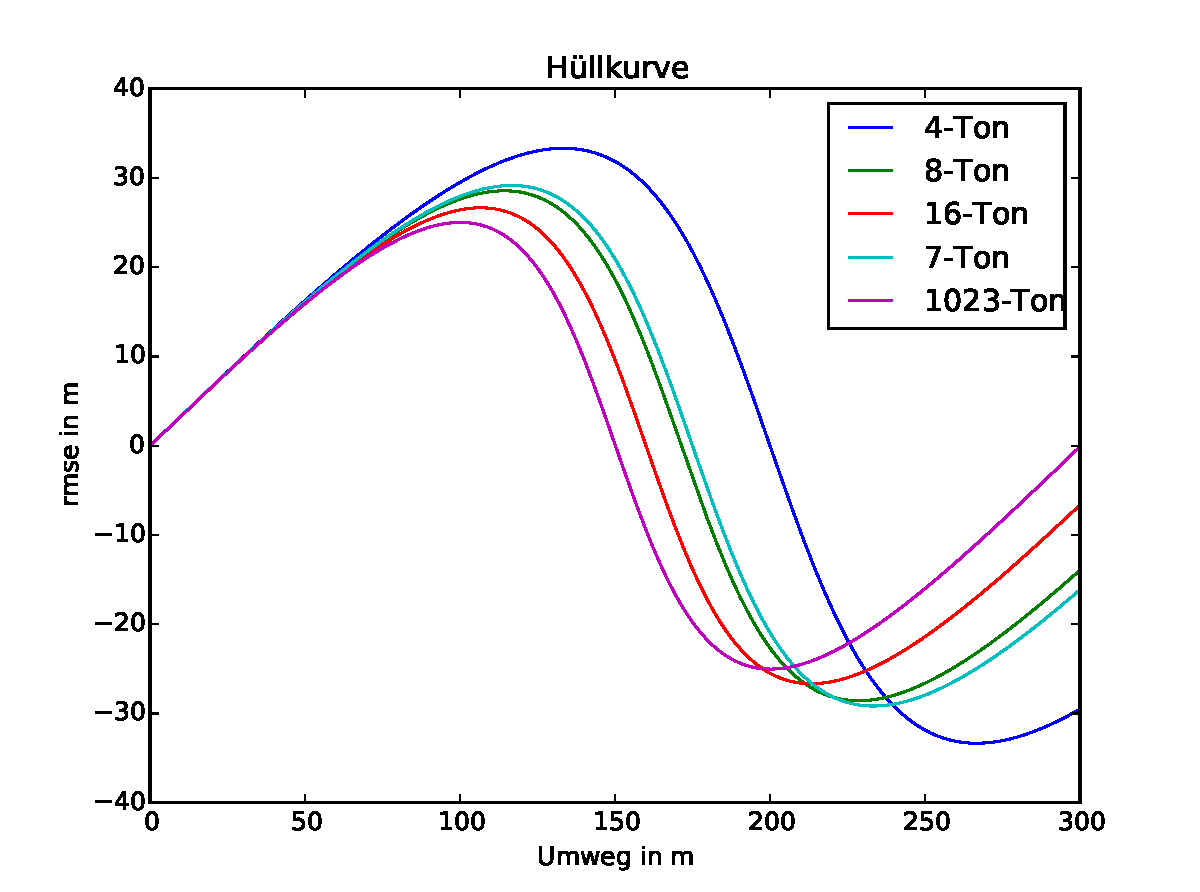
\includegraphics[width = 0.7\textwidth]{images/Huellkurve_ohne_Traeger}
	\caption{Mittlerer Schätzfehler durch einen zweiten Pfad, ohne Einfluss eines Phasenoffsets}
	\label{fig:HullkurveBasisband}
\end{figure}

Streng genommen ist die Abbildung \ref{fig:HullkurveBasisband} keine vollständige Hüllkurve. Erst wenn Phasenoffsets bis $\unit[180]{^\circ}$ berücksichtigt werden, wird die Einhüllende sichtbar. Der besseren Übersichtlichkeit halber werden in dieser Abbildung keine Phasenoffsets abgebildet. Es ist zu erkennen, dass der Fehler sich periodisch über dem Umweg wiederholt. Die Periodendauer wird jedoch mit steigender Subträgerzahl kleiner. Diese Periodizität ist im Abstand zweier benachbarter Abtastwerte begründet, welcher durch $T_{chip}=\nicefrac[]{1}{\gls{symb:B}}$ gegeben ist. Ist das Signal des Umwegpfads um genau einen Abtastwert länger verzögert, als das Signal des \gls{LOS}, haben dessen Subträger eine um $\unit[180]{^\circ}$ verdrehte Phasenlage. Aus Abbildung \ref{fig:MehrwegeZeiger} kann entnommen werden, dass bei einer solchen Phasenlage des Umwegs zum \gls{LOS}, kein Phasenfehler entsteht. Lediglich der Betrag des Umwegs interferiert destruktiv mit dem \gls{LOS}. Deshalb durchläuft die Kurve an dieser Stelle den Nullpunkt. Um die Unterschiede der Periodendauern $T_{chip}$ der Signale zu erklären, müssen die Spektren genauer betrachtet werden. In diesen kann erkannt werden, dass die Bandbreite, je nach Subträgerverteilung variiert. Lediglich die $m$-Sequenz mit 1023 Subträgern hat eine Bandbreite von $\unit[2]{MHz}$ und hat deshalb ihren Nulldurchlauf bei $\unit[150]{m}$.
Des Weiteren ist festzustellen, dass sich der maximale Fehler mit steigender Subträgerzahl verringert. Das zeigt, dass Mehrwegefehler durch Mittelung reduziert werden können. Jedoch liegen diese bei dem Testsignal mit der höchsten Anzahl an Subträgern noch über $\unit[20]{m}$. Ein solcher Fehler in der Distanzschätzung ist für Ortungssysteme nicht tolerabel. 

Als nächstes soll der Einfluss von Phasenoffsets genauer untersucht werden. 
\begin{figure}[htbp]
	\centering
	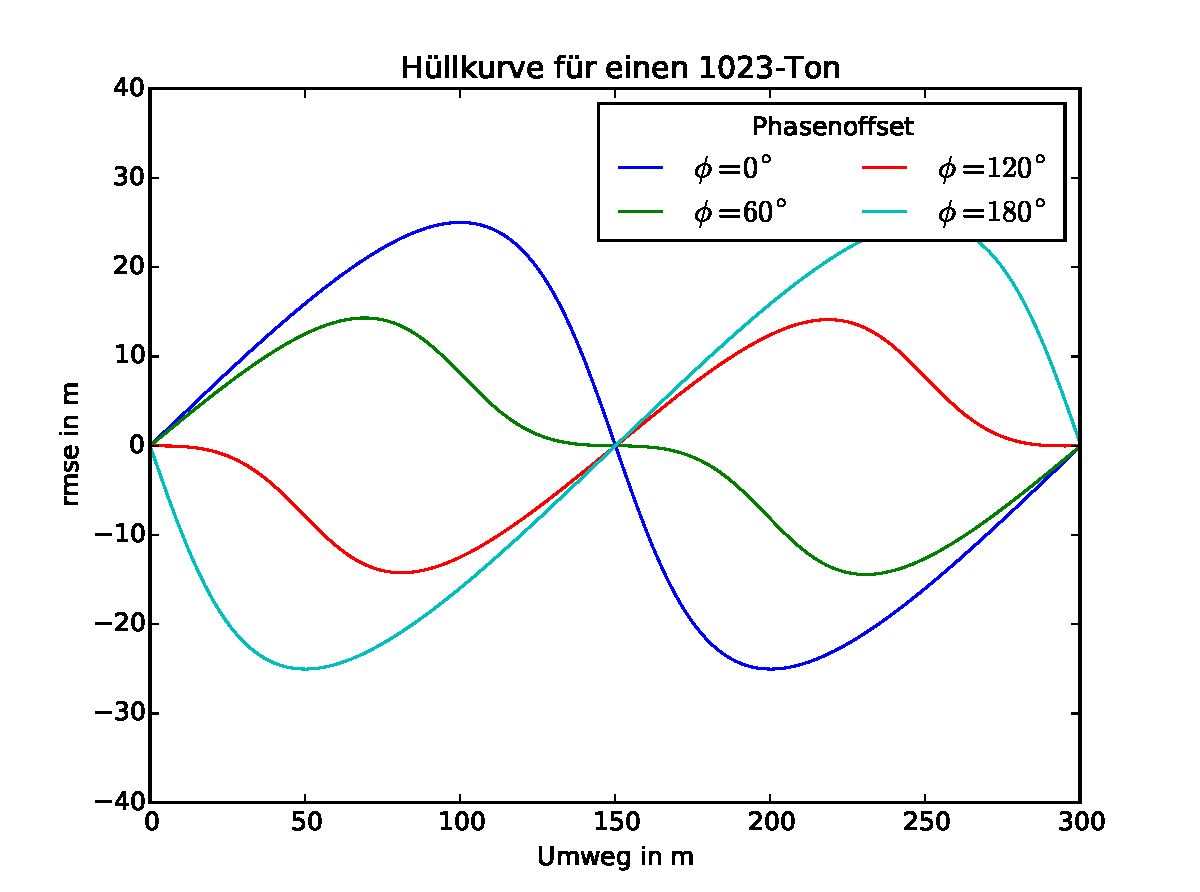
\includegraphics[width = 0.7\textwidth]{images/Hullkurven_1023Ton_ohneTraeger}
	\caption{Hüllkurve einer $m$-Sequenz unter Einfluss von Phasenoffsets}
	\label{fig:Hüllkurve mit Phasenoffset}
\end{figure}
In Abbildung \ref{fig:Hüllkurve mit Phasenoffset} ist eine Hüllkurve für einen 1023-Ton und vier Phasenoffsets zu sehen. Es ist zu erkennen, dass durch zufällige Phasendrehungen, durch Objekte an denen das Signal des zweite Pfad reflektiert wird, die maximalen Fehler zwischen den Fehlerkurven für $\unit[0]{^\circ}$ und $\unit[180]{^\circ}$ liegen. Wenn die Trägerfrequenz \gls{symb:fc} mitberücksichtigt wird, verändern sich die Hüllkurven jedoch leicht. 

\begin{figure}[htbp]
	\centering
	\makebox[\textwidth][c]{\begin{tabular}{cccc}
		\subfloat[4-Ton]{\includegraphics[width = 0.5\textwidth]{images/Hullkurven_4_Ton}} &
		\subfloat[16-Ton]{\includegraphics[width = 0.5\textwidth]{images/Hullkurven_16_Ton}}
	\end{tabular}}
	\caption{Hüllkurven zweier Hadamard-Sequenzen mit einer Trägerfrequenz \gls{symb:fc}$=\unit[868]{MHz}$ und unter Einfluss von Phasenoffsets}
	\label{fig:Hüllkurve mit Träger}
\end{figure}	

Der Zeiger des Umwegpfades aus Abbildung \ref{fig:MehrwegeZeiger} dreht sich aufgrund der Trägerfrequenz nun deutlich schneller. Dadurch umrundet dieser Zeiger für jeden gewanderten Meter etwa $2,8$ mal die Spitze des \gls{LOS}-Zeigers. Diese Periodizität von ungefähr $\unit[35]{cm}$ ist in Abbildung \ref{fig:Hüllkurve mit Träger} deutlich zu erkennen. Es ist ersichtlich , dass sich am maximalen Mehrwegefehler nichts geändert hat. Jedoch scheinen die Phasenoffsets keinen großen Einfluss mehr auf diesen zu haben. Um das genauer untersuchen zu können, ist im Folgenden eine Vergrößerung der Abbildung \ref{fig:Hüllkurve mit Träger} zu sehen. 

\begin{figure}[htbp]
	\centering
	\makebox[\textwidth][c]{\begin{tabular}{cccc}
		\subfloat[4-Ton]{\includegraphics[width = 0.5\textwidth]{images/Hullkurven_4_Ton_zoom}} &
		\subfloat[16-Ton]{\includegraphics[width = 0.5\textwidth]{images/Hullkurven_16_Ton_zoom}}
	\end{tabular}}
	\caption{Hüllkurven zweier Hadamard-Sequenzen mit einer Trägerfrequenz von $\unit[868]{MHz}$ und unter Einfluss von Phasenoffsets}
	\label{fig:Hüllkurve mit Träger gezoomt}
\end{figure}

Anhand dieser Vergrößerungen wird sichtbar, dass die Fehlerkurven später einsetzen. Somit verschiebt der Phasenoffset die Kurven nur und beeinflusst den maximalen Fehler nicht. 


\subsection{Auswertung des \gls{LuR}-Schätzers}

Beim \gls{LuR}-Schätzer war die Annahme, dass, durch Verwendung unterschiedlicher Abstände zwischen den Subträgern, zur Phasendifferenzbildung eine höhere Genauigkeit erzielt werden kann. Im Abschnitt \ref{chap5.1.2:LundR Auswertung} wurde bereits festgestellt, dass dieser Schätzer eine suboptimale Vereinfachung trifft, welche nicht auf die hier verwendeten Signale zutrifft. Dadurch müssen alle Subträger im Schätzer zunächst skaliert werden. Folglich wird auch der Mehrwegefehler, mit denen die Subträger vorher behaftet sind, skaliert. Es stellt sich die Frage, wie sich diese Maßnahme auf die Hüllkurven auswirkt. Zunächst wird jedoch, wie in Abschnitt \ref{chap:5.2.1:gemittelte Phasendifferenz} der mittlere Schätzfehler bei Mehrwegeausbreitung ohne Einfluss von Trägerfrequenz oder Phasenoffsets betrachtet.
 
\begin{figure}[htbp]
	\centering
	\includegraphics[width = 0.7\textwidth]{images/LuR_Huellkurve_ohne_Traeger}
	\caption{Mittlerer Schätzfehler durch einen 2. Pfad, ohne Einfluss eines Phasenoffsets}
	\label{fig:LuRHullkurveBasisband}
\end{figure}

Die Periodendauer des Fehlers der unterschiedlichen Signale wird bei diesem Schätzer nicht kleiner. Dies deutet schon auf ein fehlerhaftes Verhalten des Schätzers hin. 
Der maximale Fehler dieses Schätzverfahrens nimmt zwar auch mit zunehmender Subträgerzahl ab, verglichen mit dem gemittelten-Phasendifferenz-Schätzer, jedoch in einem viel geringerem Maß. Zwischen 8-Ton und 1023-Ton ist kaum noch eine Verbesserung zu sehen. Die getroffenen Maßnahmen, um diesen Schätzer an die Signale anzupassen, scheinen die Leistungsfähigkeit beeinträchtigt zu haben. Nicht nur an der Lage des Nulldurchlaufs der Kurven für die Signale, sondern auch an den Kurven mit Phasenoffsets, kann ein ungewöhnliches Verhalten des Schätzfehlers festgestellt werden. In Abbildung \ref{fig:LuRHüllkurve mit Phasenoffset} ist zu erkennen, dass die Periodendauer des Fehlers für unterschiedliche Phasenoffsets nicht bei den selben Verzögerungen liegen, wie es beim gemittelten-Phasendifferenz-Schätzers der Fall war. In Abbildung \ref{fig:HüllkurvenLuR-Had} ist an dieser Stelle eine Verzerrung zu sehen.

\begin{figure}[htbp]
	\centering
	\includegraphics[width = 0.7\textwidth]{images/LuR_Hullkurven_1023_ohneTraeger}
	\caption{Hüllkurve einer m-Sequenz unter Einfluss von Phasenoffsets}
	\label{fig:LuRHüllkurve mit Phasenoffset}
\end{figure}
 
Eine weitere Beobachtung ist, dass der maximale \gls{rmse} in der zweiten Periode kleiner wird. Sehr deutlich kann dieser Effekt bei dem 1023-Ton, in Abbildung \ref{fig:LuRHüllkurve mit Phasenoffset} erkannt werden. Die Begründung hierfür ist der zu lange Umwegpfad. Der \gls{LuR}-Schätzer hat einen deutlich kleineren Eindeutigkeitsbereich als der gemittelte-Phasendifferenz-Schätzer, sodass der Umwegpfad diesen nach der ersten Periode verlässt.

\begin{figure}
	\makebox[\textwidth][c]{\begin{tabular}{ccc}
		\subfloat[4-Ton]{\includegraphics[width = 0.5\textwidth]{images/Hullkurven_4_LuR}} &
		\subfloat[16-Ton]{\includegraphics[width = 0.5\textwidth]{images/Hullkurven_16_LuR}}
		\end{tabular}}
		\caption{Hüllkurven des \gls{LuR} Schätzers}
		\label{fig:HüllkurvenLuR-Had}
\end{figure}				

Dieser Schätzer liefert für die hier verwendeten Signale kein besseres Auflösungsvermögens des Mehrwegekanals. Um bessere Ergebnisse zu erzielen, müssen Signale verwendet werden, die die Bedingungen für das Verwenden der Gleichung \eqref{eq:Approximation} erfüllen. Die nachträgliche Skalierung der Subträgergewichte führt zu einem unerwarteten Verhalten.  

\subsection{Auswertung der Subraumalgorithmen}

Wie bereits im \gls{AWGN}-Fall erwähnt, liefern \gls{MUSIC} und \gls{ESPRIT} ähnliche Ergebnisse. 
\begin{figure}
	\makebox[\textwidth][c]{\begin{tabular}{ccc}
		\subfloat[4-Ton]{\includegraphics[width = 0.5\textwidth]{images/Hullkurven_4Ton_ESPRIT}} &
		\subfloat[7-Ton]{\includegraphics[width = 0.5\textwidth]{images/Hullkurven_7Ton_ESPRIT}}
	\end{tabular}}
	\caption{Mehrwegehüllkurven einer Hadamard- und einer $m$-Sequenz}
	\label{fig:ESPIT_Mehrwege}
\end{figure}
Da diese Algorithmen die Pfade trennen können, ist es nicht weiter verwunderlich, dass bei Mehrwegeausbreitung kein Schätzfehler entsteht, wie in Abbildung \ref{fig:ESPIT_Mehrwege}. 
Es stellt sich jedoch die Frage, ob diese Eigenschaft, die Pfade trennen zu können, auch bei schlechten Signal-Rausch-Verhältnissen bestehen bleibt. 

\subsection{Bewertung bei Mehrwegeausbreitung}
In den vorangegangenen Auswertungen stellte sich heraus, dass Mittelungsverfahren den Schätzfehler in einem Mehrwegekanal durch Mehrtonsignale reduzieren können, jedoch diese immer noch zu groß bleiben. Der maximale Fehler war bei dem gemittelten-Phasendifferenz-Schätzer in Kombination mit der $m$-Sequenz mit 1023 Subträgern am kleinsten, liegt allerdings immer noch über $\unit[20]{m}$. Es hat sich auch herausgestellt, dass der \gls{LuR}-Schätzer, aufgrund seiner Modifikationen für die verwendeten Signale, schlechter als der gemittelte-Phasendifferenz-Schätzer abschneidet. Allerdings zeigt er vielversprechende Tendenzen und sollte nochmals mit geeigneten Signalen und einer geeigneten Impulsformung genauer untersucht werden.    
Die Subraummethoden erweisen sich als die besten Verfahren, Parameter in Mehrwegekanälen zu schätzen. 
Es muss allerdings eine Betrachtung des gesamten Kanals durchgeführt werden, um eine Aussage über die Leistungsfähigkeit zu treffen. 

\section{Betrachtung des gesamten Kanals}
Die Auswertung bei Mehrwegeausbreitung zeigt, dass nur die Subraummethoden handhabbare Fehler produzieren. Mittelungsverfahren, wie sie hier vorgestellt wurden, sind hingegen keine gute Lösung für ein Ortungssystem, dass mehrwegerobust sein soll. 
Zusätzlich stellt sich heraus, dass die $m$-Sequenz mit 7 Subträgern das beste Verhalten bei \gls{AWGN} unter Einsatz der Subraummethoden aufweist. Deshalb soll in diesem Abschnitt der \gls{ESPRIT}- und \gls{MUSIC}-Algorithmus unter Einfluss des gesamten Kanalmodells mit einem 7-Ton untersucht werden. Bei der Untersuchung der Subraummethoden im \gls{AWGN}-Fall konnten Fehler erst ab einem \nicefrac[]{\gls{symb:C}}{\gls{symb:N0}} von $\unit[96]{dB-Hz}$ festgestellt werden. Deshalb wird in den folgenden Betrachtungen der \gls{rmse} für vier \nicefrac[]{\gls{symb:C}}{\gls{symb:N0}}-Werte berechnet. Diese Werte entsprechen den, mit der Bandbreite $\unit[4]{MHz}$ normierten, Signal-Rausch-Verhältnissen $\unit[30]{dB}$, $\unit[20]{dB}$, $\unit[10]{dB}$ und $\unit[0]{dB}$. Im reinen \gls{AWGN}-Fall haben die Algorithmen Fehler im Bereich $\unit[0]{m}-\unit[1,5]{m}$ erzeugt. 

\begin{figure}[htbp]
	\centering
	\makebox[\textwidth][c]{\begin{tabular}{cccc}
		\subfloat[\gls{MUSIC} mit 7-Ton]{\includegraphics[width = 0.5\textwidth]{images/MUSIC_GesamtkanalAuswertung}} &
		\subfloat[\gls{ESPRIT} mit 7-Ton]{\includegraphics[width = 0.5 \textwidth]{images/ESPRIT_GesamtkanalAuswertung}}
	\end{tabular}}
	\caption{Auswertung des Einflusses des gesamten Kanalmodells}
	\label{fig:GesamtkanalAuswertung}
\end{figure}
In Abbildung \ref{fig:GesamtkanalAuswertung} ist der Fehler bei Mehrwegeausbreitung und schlechten Signal-Rausch-Verhältnissen aufgetragen. Man sieht, dass der Fehler nun erheblich größer als im Vergleich zum reinen \gls{AWGN}-Fall geworden ist. Für einen Umwegpfad, länger als $\unit[80]{m}$, flacht der Fehler jedoch wieder ab und liegt sogar bei $\unit[66]{dB-Hz}$ unter $\unit[5]{m}$. Davor kann der maximale Fehler bis zu $\unit[20]{m}$ groß werden. Es ist aber auch zu erkennen, dass alle $\unit[10]{dB-Hz}$, die das \nicefrac[]{\gls{symb:C}}{\gls{symb:N0}} besser wird, der Fehler sich fast halbiert. 
Es zeigt sich, dass bei kurzen Umwegpfaden und schlechten Signal-Rausch-Verhältnissen, die Fehler nicht mehr tolerierbar sind. Verbessert sich jedoch das \nicefrac[]{\gls{symb:C}}{\gls{symb:N0}} um nur $\unit[10]{dB-Hz}$ erreicht man wieder akzeptable Fehlerwerte. Es muss jedoch beachtet werden, dass es Signalformen gibt, welche die Energie, bezüglich einer optimalen \gls{CRLB} noch besser Verteilen könnten. Zudem wird die \gls{CRLB} durch die Impulsformung verschlechtert, da die Multiplikation mit einer Sinc-Funktion im Frequenzbereich die äußeren Subträger nach unten skaliert. Es wäre denkbar hier eine Sinc-Funktion als Modulationsimpuls zu verwenden, um im Frequenzbereich eine Multiplikation mit einem Rechteck zu bewerkstelligen.



\chapter{Zusammenfassung und Ausblick}
\label{chap:Schluss}

Im Rahmen dieser Arbeit wurden Mehrtonsignale zur robusten Distanzschätzung untersucht. Dafür mussten Schätzverfahren gefunden und implementiert werden, welche den Informationsgewinn über den Kanal, durch zusätzliche Subträger, ausnutzen können. Robust ist eine Distanzschätzung, wenn selbst bei einem stark gestörten Kanal, wie bei Mehrwegeausbreitung, ein geringer Schätzfehler entsteht. Es wurden fünf Signale mit verschiedenen Subträgerverteilungen und zwei Schätzstrategien, mit jeweils zwei Schätzalgorithmen untersucht. Die erste Strategie, basierend auf Mittelung, beinhaltet einen Schätzer, der Phasendifferenzen zwischen allen benachbarten Subträger bestimmt und anschließend einen Mittelwert bildet. Der zweite Schätzer, welcher dieselbe Strategie verfolgt, wurde von Luise und Reggiannini vorgestellt. Dieser Schätzer verbessert die Genauigkeit der Schätzung, indem er nicht nur Differenzen benachbarter Träger, sondern zwischen allen Trägern bestimmt. Dadurch verkleinert sich jedoch der Eindeutigkeitsbereich der Schätzung. Die Genauigkeit und das \gls{SNR} verbessern sich hingegen. Bei der Verwendung dieses Verfahrens wird eine Vereinfachung getroffen, die nicht auf alle Signalformen zutrifft. Folglich ist dieser Schätzer nicht für alle Signalformen geeignet. Beide Verfahren konnten, mithilfe der zusätzlichen Subträger, Schätzfehler im Mehrwegekanal verringern. Beim Mehrwegekanal ist der Fehler jedoch immer noch zu groß um in realen Systemen eingesetzt zu werden. Der \gls{LuR}-Schätzer musste für die, in dieser Arbeit verwendeten Signale angepasst werden, was seine Leistung minderte. Es ist zu Überlegen, diesen Schätzer mit geeigneten Signalen und einer geeigneten Impulsformung erneut zu Simulieren. 
Die zweite Strategie basiert auf der Zerlegung der Kanalschätzung in einen Signal- und einen Rauschraum. Dadurch, dass Signal- und Rauschanteil getrennt werden, können die zu schätzenden Parameter direkt aus dem Signalraum extrahiert werden. Der MUSIC-Algorithmus erzeugt einen Suchvektor (Steringvektor), welcher alle Verzögerungen durchläuft, und multipliziert ihn mit dem Rauschraum. Entsteht bei der Multiplikation eine Nullstelle, ist die Laufzeit zum gesuchten Vektor gefunden. Dieser Suchprozess ist jedoch rechenaufwendig. Einen anderen Ansatz verfolgt das ESPRIT-Verfahren. Dieses teilt den Signalraum in zwei Frequenzabschnitte, welche durch ein least squares-Problem miteinander verknüpft sind. Zur Bestimmung des gesuchten Parameters muss dieses least squares-Problem gelöst werden.  
Die Methoden, basierend auf einer Zerlegung in Subräume, erreichen zwar nur für einen 7-Ton, im \gls{AWGN}-Kanal die untere Fehlerschranke, können den Mehrwegekanal jedoch sehr gut auflösen. 
Abschließend wurde geschlussfolgert, dass die Subraummethoden in Kombination mit Mehrträgersignalen, bei welchen alle Subträger gleich gewichtet sind, die besten Ergebnisse erzielen. Die Anzahl der Subträger sollte allerdings nicht zu groß gewählt werden, da bei einem kleinem Signal-Rausch-Verhältnis für solche Signale die untere Fehlerschranke nicht erreicht werden kann. Bei der Auswertung wurde mit dem MUSIC-Algorithmus in Kombination einer 7-Träger $m$-Sequenz die besten Ergebnisse erzielt. 


Die Ergebnisse der abschließenden Auswertung sind vielversprechend, da selbst bei einem, im Bezug auf die \gls{CRLB}, nicht idealem Signal, Mehrwegefehler minimiert werden konnten. Der zu beobachtende Schätzfehler ist im Bereich von schlechten Signal-Rausch-Verhältnissen und kurzen Umwegpfaden stark angestiegen. Zudem sollte im Hinterkopf behalten werde, dass das Verhältnis des \gls{SNR} vom \gls{LOS} zu dem des Umwegpfades konstant gehalten wurde. Dies entspricht nicht der Realität, da das \gls{SNR} des Umwegpfades ebenfalls mit zunehmender Distanz abnimmt.  
Es bietet sich an in zukünftigen Arbeiten an der Optimierung der Signalform zu arbeiten, da sich herausgestellt hat, dass unterschiedlich stark gewichtete Subträger, für die in dieser Arbeit untersuchten Schätzer, nicht sehr geeignet sind. Zudem muss auch auf die Impulsformung in zukünftigen Simulationen geachtet werden, da sich herausgestellt hat, dass ein Rechteckimpuls die Gewichte der Subträger verändert. Es wäre denkbar an dieser Stelle eine Sinc-Funktion zur Impulsformung zu verwenden.
Des Weiteren sollte eine Verifizierung der Ergebnisse in einer realen Umgebung stattfinden, da Faktoren die in diesen Betrachtungen vernachlässigt wurden Einflüsse auf die Ergebnisse haben können, wie beispielsweise die zusätzliche Dämpfung des Umwegpfades durch die Reflexion.



\printglossary[style=altlist,title=Glossar]

% Anhang (Bibliographie darf im deutschen nicht in den Anhang!)
\nocite{*}
\bibliography{bib/BibtexDatabase}
\clearpage
%\addcontentsline{toc}{chapter}{Abbildungsverzeichnis}
\listoffigures
\clearpage
%\addcontentsline{toc}{chapter}{Tabellenverzeichnis}
\listoftables

% Anhang
\appendix
% \input{content/Z-Anhang-01-Herleitungen}

\chapter{Anhang}
\label{chap:Anhang}

\section{Elektronischer Anhang (auf CD)}

\begin{itemize}
	\item Python-Skripte der Simulationsumgebung
	\item PDF-Version der vorliegenden Arbeit
	\item Latex-Version der vorliegenden Arbeit
	\item PDF's der Verwendeten Literatur 
\end{itemize}


%% Dokument ENDE %%%%%%%%%%%%%%%%%%%%%%%%%%%%%%%%%%%%%%%%%%%%%%%%%%%%%%%%%%
\end{document}

